% =====================================================================
%  BÁO CÁO TỔNG KẾT ĐỀ TÀI NCKH SINH VIÊN — mã số SV2026-474
%  Trình bày theo "Phụ lục hướng dẫn viết báo cáo tổng kết" (PKHCN):
%    A4; Times New Roman 13; giãn dòng 1,4 (trong khoảng 1,3–1,5);
%    lề trái 3 cm, lề trên/dưới/phải 2 cm.
%  Biên dịch:  pdflatex main && pdflatex main && pdflatex main
%  (font Times: VnNimbusRomanNo9L của gói vntex — bản cùng metric với
%   Times New Roman, có đủ dấu tiếng Việt.)
% =====================================================================
\documentclass[a4paper,12pt,oneside]{report}
\usepackage[fontsize=13pt]{scrextend}

\usepackage[T5]{fontenc}
\usepackage[utf8]{inputenc}
\usepackage[vietnamese]{babel}
\usepackage{mathptmx}

\usepackage[a4paper,left=3cm,right=2cm,top=2cm,bottom=2cm,
            includefoot,footskip=1cm]{geometry}
\usepackage{setspace}
\setstretch{1.4}

\usepackage{amsmath,amssymb}
\usepackage{graphicx}
\usepackage{booktabs,multirow,array,tabularx,longtable,makecell}
\usepackage[table]{xcolor}
\usepackage{float}
\usepackage[font=small,labelfont=bf,labelsep=period,justification=centering]{caption}
\usepackage{subcaption}
\usepackage{enumitem}
\usepackage{fancyhdr}
\usepackage{titlesec}
\usepackage[titles]{tocloft}
\usepackage{pdfpages}
\usepackage{tikz}
\usetikzlibrary{arrows.meta,positioning,shapes.geometric,fit,calc,backgrounds}
\usepackage{listings}
\usepackage{xurl}
\usepackage[unicode,hidelinks]{hyperref}

% =====================================================================
%  THÔNG TIN CHUNG — dùng chung cho báo cáo, tóm tắt, poster, slide.
%  Sửa ở ĐÂY một lần, mọi tài liệu tự cập nhật khi biên dịch lại.
%  Nguồn: Thuyết minh BM02 (mã số SV2026-474).
% =====================================================================
\newcommand{\tendetai}{Máy bay không người lái tự động theo dõi con người bằng trí tuệ nhân tạo}
\newcommand{\TENDETAI}{MÁY BAY KHÔNG NGƯỜI LÁI TỰ ĐỘNG THEO DÕI CON NGƯỜI BẰNG TRÍ TUỆ NHÂN TẠO}
\newcommand{\madetai}{SV2026-474}
\newcommand{\truong}{Trường Đại học Công nghệ Kỹ thuật Thành phố Hồ Chí Minh}
\newcommand{\TRUONG}{TRƯỜNG ĐH CÔNG NGHỆ KỸ THUẬT TP.HCM}
\newcommand{\khoa}{Đào tạo tiên tiến}
\newcommand{\bomon}{Công nghệ kỹ thuật máy tính}
\newcommand{\nganhhoc}{Công nghệ kỹ thuật máy tính}
\newcommand{\nhomnganh}{Kỹ thuật và Công nghệ}
\newcommand{\loaihinh}{Ứng dụng}

\newcommand{\chunhiem}{Huỳnh Lê Thành Nhân}
\newcommand{\mssvchunhiem}{24119068}
\newcommand{\emailchunhiem}{24119068@student.hcmute.edu.vn}
\newcommand{\dienthoai}{0937395656}

\newcommand{\thanhvien}{Trịnh Trần Quốc Bảo}
\newcommand{\mssvthanhvien}{24119016}
\newcommand{\emailthanhvien}{24119016@student.hcmute.edu.vn}
\newcommand{\dienthoaithanhvien}{0962924006}

\newcommand{\gvhd}{PGS.TS. Lê Mỹ Hà}
\newcommand{\emailgvhd}{halm@hcmute.edu.vn}

% Thông tin cá nhân (chủ nhiệm đề tài cung cấp 16/09/2026).
\newcommand{\gioitinh}{Nam}
\newcommand{\dantoc}{Kinh}
\newcommand{\ngaysinh}{14/08/2006}
\newcommand{\lopchunhiem}{24119FIE4}
\newcommand{\lopthanhvien}{24119FIE4}
\newcommand{\namthu}{3}
\newcommand{\sonamdaotao}{4}

\newcommand{\thangnam}{09/2026}



% ---------- chú thích: tên hình dưới hình, tên bảng trên bảng ----------
\captionsetup[table]{position=top,skip=4pt}
\captionsetup[figure]{position=bottom,skip=6pt}
\addto\captionsvietnamese{%
  \renewcommand{\figurename}{Hình}%
  \renewcommand{\tablename}{Bảng}%
  \renewcommand{\contentsname}{MỤC LỤC}%
  \renewcommand{\listtablename}{DANH MỤC BẢNG BIỂU}%
  \renewcommand{\listfigurename}{DANH MỤC HÌNH ẢNH}%
  \renewcommand{\bibname}{TÀI LIỆU THAM KHẢO}%
  \renewcommand{\chaptername}{CHƯƠNG}%
  \renewcommand{\appendixname}{PHỤ LỤC}%
}
\renewcommand{\thefigure}{\thechapter.\arabic{figure}}
\renewcommand{\thetable}{\thechapter.\arabic{table}}

% ---------- tiêu đề chương / mục ----------
\titleformat{\chapter}[display]{\normalfont\large\bfseries\centering}
  {\chaptertitlename\ \thechapter}{4pt}{\large\MakeUppercase}
\titlespacing*{\chapter}{0pt}{0pt}{18pt}
\titleformat{\section}{\normalfont\normalsize\bfseries}{\thesection}{0.6em}{}
\titleformat{\subsection}{\normalfont\normalsize\bfseries\itshape}{\thesubsection}{0.6em}{}
\titleformat{\subsubsection}{\normalfont\normalsize\itshape}{\thesubsubsection}{0.6em}{}
\titlespacing*{\section}{0pt}{10pt}{4pt}
\titlespacing*{\subsection}{0pt}{8pt}{3pt}
\titlespacing*{\subsubsection}{0pt}{6pt}{2pt}
\setcounter{secnumdepth}{3}
\setcounter{tocdepth}{2}

% chương không đánh số (Mở đầu, Kết luận, TLTK)
\newcommand{\chuongkhongso}[1]{%
  \chapter*{\centering\large\bfseries\MakeUppercase{#1}}%
  \addcontentsline{toc}{chapter}{\MakeUppercase{#1}}%
  \markboth{#1}{#1}}

% ---------- mục lục ----------
\renewcommand{\cftchapfont}{\bfseries}
\renewcommand{\cftchappagefont}{\bfseries}
\renewcommand{\cftchapleader}{\cftdotfill{\cftdotsep}}
\renewcommand{\cftchappresnum}{CHƯƠNG }
\setlength{\cftchapnumwidth}{6.2em}
\renewcommand{\cftfigpresnum}{Hình }
\renewcommand{\cfttabpresnum}{Bảng }
\setlength{\cftfignumwidth}{5em}
\setlength{\cfttabnumwidth}{5em}
\setlength{\cftbeforechapskip}{4pt}

% ---------- đầu/chân trang ----------
\pagestyle{fancy}
\fancyhf{}
\fancyfoot[C]{\thepage}
\renewcommand{\headrulewidth}{0pt}
\fancypagestyle{plain}{\fancyhf{}\fancyfoot[C]{\thepage}\renewcommand{\headrulewidth}{0pt}}

\setlist{itemsep=1pt,topsep=3pt,parsep=0pt,leftmargin=1.6em}
\setlength{\parindent}{1cm}
\setlength{\parskip}{3pt}

% ---------- tiện ích ----------
\newcommand{\sd}{SteadyDet-N}
\newcommand{\ms}[2]{#1\,{\footnotesize$\pm$#2}}
\newcommand{\hl}[1]{\textbf{#1}}
\definecolor{xanh}{HTML}{2A78D6}
\definecolor{cam}{HTML}{EB6834}
\definecolor{xam}{HTML}{8A8986}
\definecolor{nen}{HTML}{EEF4FC}
\lstset{basicstyle=\ttfamily\footnotesize,breaklines=true,frame=single,
        columns=fullflexible,keepspaces=true,backgroundcolor=\color{gray!6}}
\graphicspath{{../hinh/}}

\begin{document}

% ====================== PHẦN ĐẦU ======================
\pagenumbering{gobble}
% ---------------- Mẫu PL01: Trang bìa chính ----------------
\thispagestyle{empty}
\begin{tikzpicture}[remember picture,overlay]
  \draw[line width=2.2pt] ($(current page.north west)+(2.6cm,-1.6cm)$) rectangle ($(current page.south east)+(-1.6cm,1.6cm)$);
  \draw[line width=0.6pt] ($(current page.north west)+(2.75cm,-1.75cm)$) rectangle ($(current page.south east)+(-1.75cm,1.75cm)$);
\end{tikzpicture}
\begin{center}
\setstretch{1.2}
{\large BỘ GIÁO DỤC VÀ ĐÀO TẠO}\\[2pt]
{\large\bfseries \TRUONG}\\[-2pt]
\rule{5cm}{0.6pt}

\vspace{3.2cm}
{\LARGE\bfseries BÁO CÁO TỔNG KẾT}\\[14pt]
{\Large\bfseries ĐỀ TÀI NGHIÊN CỨU KHOA HỌC CỦA SINH VIÊN}

\vspace{1.8cm}
\begin{minipage}{0.9\textwidth}\centering\setstretch{1.25}
{\LARGE\bfseries \TENDETAI}
\end{minipage}

\vspace{0.8cm}
{\Large\bfseries Mã số: \madetai}

\vfill
\begin{tabular}{@{}l@{\hspace{0.6em}}l@{}}
\large\bfseries Chủ nhiệm đề tài: & \large \chunhiem
\end{tabular}

\vspace{2.6cm}
{\large\bfseries TP Hồ Chí Minh, \thangnam}
\end{center}
\clearpage

% ---------------- Mẫu PL02: Trang bìa phụ ----------------
\thispagestyle{empty}
\begin{tikzpicture}[remember picture,overlay]
  \draw[line width=2.2pt] ($(current page.north west)+(2.6cm,-1.6cm)$) rectangle ($(current page.south east)+(-1.6cm,1.6cm)$);
  \draw[line width=0.6pt] ($(current page.north west)+(2.75cm,-1.75cm)$) rectangle ($(current page.south east)+(-1.75cm,1.75cm)$);
\end{tikzpicture}
\begin{center}
\setstretch{1.2}
{\large BỘ GIÁO DỤC VÀ ĐÀO TẠO}\\[2pt]
{\large\bfseries \TRUONG}\\[-2pt]
\rule{5cm}{0.6pt}

\vspace{1.6cm}
{\LARGE\bfseries BÁO CÁO TỔNG KẾT}\\[14pt]
{\Large\bfseries ĐỀ TÀI NGHIÊN CỨU KHOA HỌC CỦA SINH VIÊN}

\vspace{1.4cm}
\begin{minipage}{0.9\textwidth}\centering\setstretch{1.25}
{\LARGE\bfseries \TENDETAI}
\end{minipage}

\vspace{0.6cm}
{\Large\bfseries Mã số: \madetai}
\end{center}

\vspace{1.2cm}
\begin{center}
\setstretch{1.5}
\begin{tabular}{@{}p{0.92\textwidth}@{}}
\textbf{Thuộc nhóm ngành khoa học:} \nhomnganh\\
\textbf{SV thực hiện:} \chunhiem \hfill \textbf{Nam, Nữ:} \gioitinh\\
\textbf{Dân tộc:} \dantoc\\
\textbf{Lớp, khoa:} \lopchunhiem, Khoa \khoa\\
\textbf{Năm thứ:} \namthu\,/\,\textbf{Số năm đào tạo:} \sonamdaotao\\
\textbf{Ngành học:} \nganhhoc\\[2pt]
\textit{(SV chịu trách nhiệm chính thực hiện đề tài: \chunhiem)}\\[6pt]
\textbf{Thành viên:} \thanhvien{} (MSSV \mssvthanhvien)\\[6pt]
\textbf{Người hướng dẫn:} Phó Giáo sư, Tiến sĩ Lê Mỹ Hà
\end{tabular}
\end{center}

\vfill
\begin{center}
{\large\bfseries TP Hồ Chí Minh, \thangnam}
\end{center}
\clearpage


\pagenumbering{roman}
\setcounter{page}{1}
\begin{singlespace}
\tableofcontents
\clearpage
\phantomsection\addcontentsline{toc}{chapter}{DANH MỤC BẢNG BIỂU}
\listoftables
\clearpage
\phantomsection\addcontentsline{toc}{chapter}{DANH MỤC HÌNH ẢNH}
\listoffigures
\end{singlespace}
% ---------------- Danh mục từ viết tắt (xếp theo bảng chữ cái) ----------------
\chapter*{\centering\large\bfseries DANH MỤC CÁC TỪ VIẾT TẮT}
\addcontentsline{toc}{chapter}{DANH MỤC CÁC TỪ VIẾT TẮT}
\begin{singlespace}
\renewcommand{\arraystretch}{1.18}
\begin{longtable}{@{}p{2.8cm}p{6.1cm}p{6.1cm}@{}}
\toprule
\textbf{Viết tắt} & \textbf{Tiếng Anh} & \textbf{Nghĩa tiếng Việt}\\
\midrule\endhead
AP & Average Precision & Độ chính xác trung bình\\
AR & Average Recall & Độ phủ trung bình\\
CIoU & Complete Intersection over Union & Chỉ số chồng lấp đầy đủ\\
CNN & Convolutional Neural Network & Mạng nơ-ron tích chập\\
COCO & Common Objects in Context & Bộ dữ liệu COCO\\
CPU & Central Processing Unit & Bộ xử lý trung tâm\\
CSP & Cross Stage Partial & Kết nối từng phần liên tầng\\
DFC & Dataflow Compiler & Trình biên dịch luồng dữ liệu (Hailo)\\
EKF & Extended Kalman Filter & Bộ lọc Kalman mở rộng\\
FCU & Flight Control Unit & Bộ điều khiển bay\\
FLOPs & Floating-point Operations & Số phép tính dấu phẩy động\\
FP32 & 32-bit Floating Point & Số thực dấu phẩy động 32 bit\\
FPN & Feature Pyramid Network & Mạng kim tự tháp đặc trưng\\
FPS & Frames Per Second & Số khung hình trên giây\\
GCS & Ground Control Station & Trạm điều khiển mặt đất\\
GFLOPs & Giga FLOPs & Tỷ phép tính dấu phẩy động\\
GPS & Global Positioning System & Hệ thống định vị toàn cầu\\
GPU & Graphics Processing Unit & Bộ xử lý đồ hoạ\\
HEF & Hailo Executable Format & Tệp mô hình thực thi trên NPU Hailo\\
IMU & Inertial Measurement Unit & Khối đo lường quán tính\\
INT8 & 8-bit Integer & Số nguyên 8 bit\\
IoU & Intersection over Union & Tỷ lệ giao trên hợp\\
MAVLink & Micro Air Vehicle Link & Giao thức truyền thông cho phương tiện bay nhỏ\\
mCP & mean Corrupted Precision & AP trung bình trên ảnh bị suy giảm\\
NMS & Non-Maximum Suppression & Loại bỏ hộp không cực đại\\
NPU & Neural Processing Unit & Bộ xử lý nơ-ron chuyên dụng\\
NWD & Normalized Wasserstein Distance & Khoảng cách Wasserstein chuẩn hoá\\
OC-SORT & Observation-Centric SORT & Thuật toán theo vết đa đối tượng lấy quan sát làm trung tâm\\
ONNX & Open Neural Network Exchange & Định dạng trao đổi mạng nơ-ron mở\\
PID & Proportional–Integral–Derivative & Bộ điều khiển tỷ lệ – tích phân – vi phân\\
PTQ & Post-Training Quantization & Lượng tử hoá sau huấn luyện\\
QFL & Quality Focal Loss & Hàm mất mát tiêu điểm theo chất lượng\\
RTL & Return To Launch & Chế độ tự bay về điểm cất cánh\\
SITL & Software In The Loop & Mô phỏng phần mềm trong vòng lặp\\
SoC & System on Chip & Hệ thống trên một vi mạch\\
SORT & Simple Online and Realtime Tracking & Theo vết trực tuyến thời gian thực đơn giản\\
STAL & Small-Target-Aware Label Assignment & Gán nhãn nhận biết mục tiêu nhỏ\\
TOPS & Tera Operations Per Second & Nghìn tỷ phép tính mỗi giây\\
UAV & Unmanned Aerial Vehicle & Máy bay không người lái\\
UIB & Universal Inverted Bottleneck & Khối nút cổ chai đảo ngược tổng quát\\
USB & Universal Serial Bus & Chuẩn giao tiếp nối tiếp đa năng\\
YOLO & You Only Look Once & Họ mô hình phát hiện đối tượng một giai đoạn\\
\bottomrule
\end{longtable}
\end{singlespace}
\clearpage

% ---------------- Mẫu PL03: Thông tin kết quả nghiên cứu ----------------
\clearpage
\thispagestyle{plain}
\phantomsection\addcontentsline{toc}{chapter}{THÔNG TIN KẾT QUẢ NGHIÊN CỨU CỦA ĐỀ TÀI}
\begin{center}
\setstretch{1.15}
{BỘ GIÁO DỤC VÀ ĐÀO TẠO}\\
{\bfseries \TRUONG}\\[-3pt]
\rule{4.5cm}{0.5pt}\\[10pt]
{\large\bfseries THÔNG TIN KẾT QUẢ NGHIÊN CỨU CỦA ĐỀ TÀI}
\end{center}
\begin{spacing}{1.3}
\noindent\textbf{1. Thông tin chung:}

\noindent -- Tên đề tài: \tendetai.

\noindent -- Mã số: \madetai.

\noindent -- Chủ nhiệm đề tài: \chunhiem \hfill Mã số SV: \mssvchunhiem

\noindent -- Lớp: \lopchunhiem \hfill Khoa: \khoa

\noindent -- Thành viên đề tài:

\begin{center}
\renewcommand{\arraystretch}{1.25}
\begin{tabular}{|c|l|c|c|c|}
\hline
\textbf{STT} & \textbf{Họ và tên} & \textbf{MSSV} & \textbf{Lớp} & \textbf{Khoa}\\\hline
1 & \chunhiem & \mssvchunhiem & \lopchunhiem & \khoa\\\hline
2 & \thanhvien & \mssvthanhvien & \lopthanhvien & \khoa\\\hline
\end{tabular}
\end{center}

\noindent -- Người hướng dẫn: \gvhd{} (\emailgvhd).

\noindent\textbf{2. Mục tiêu đề tài:}
\begin{itemize}
\item Xây dựng mô hình trí tuệ nhân tạo phát hiện và nhận dạng con người theo thời gian thực từ camera gắn trên máy bay không người lái, đạt độ chính xác từ 70\% trở lên.
\item Thiết kế thuật toán theo dõi chuyển động để máy bay giữ khoảng cách và hướng bay phù hợp với người được theo.
\item Tích hợp camera -- khối xử lý ảnh -- bộ điều khiển bay thành một hệ thống hoạt động ổn định trong môi trường thực tế.
\end{itemize}

\noindent\textbf{3. Tính mới và sáng tạo:}
\begin{itemize}
\item Đề xuất mạng phát hiện người \sd{} chỉ \hl{1,17 triệu tham số và 4,6 GFLOPs}, giữ nhánh độ phân giải cao P2 (bước 4) để thấy được người ở xa, nhưng làm mỏng nhánh này để chạy được trên thiết bị biên.
\item Chỉ ra bằng đo đạc có đối chứng rằng rung động của khung máy bay làm mọi bộ phát hiện nhỏ mất 74--83\% độ chính xác, và đề xuất \hl{huấn luyện nhận biết rung}: đưa mô hình vật lý của motion blur, nhiễu cảm biến và dao động phơi sáng vào dữ liệu huấn luyện. Tỷ lệ giữ độ chính xác khi rung tăng từ \hl{16,8\% lên 36,2\%} mà \hl{không tốn thêm chi phí suy luận}; khi rung, \sd{} vượt cả bốn mô hình YOLO bản nano.
\item Xây dựng giao thức đánh giá rung VisDrone-Shake \hl{cố định seed ngẫu nhiên, lặp 3 lần và báo cáo độ lệch chuẩn}, dùng một chương trình chấm điểm duy nhất cho mọi mô hình.
\item Chứng minh trên phần cứng thật rằng tốc độ trên NPU Hailo-8L phụ thuộc vào \hl{số context} của mô hình chứ không chỉ số phép tính: \sd{} chạy \hl{nhanh hơn YOLO26-n 1,70 lần} trên cùng một chip.
\item Thiết kế lớp an toàn theo nguyên tắc \hl{người lái luôn giữ quyền chọn chế độ bay}: phần mềm chỉ đề xuất vận tốc khi máy bay đang ở chế độ GUIDED, mất mục tiêu thì đứng yên chờ, và nguyên tắc được khoá bằng kiểm thử tự động.
\end{itemize}

\noindent\textbf{4. Kết quả nghiên cứu:}
\begin{itemize}
\item Mô hình chạy INT8 trên NPU Hailo-8L đạt \hl{AP@0,5 = 0,917} (tức 91,7\%, vượt chỉ tiêu 70\%) và \hl{F1 = 0,880} (recall 0,837, precision 0,928) trên 92 khung hình bay thật ở độ cao khoảng 6\,m.
\item Toàn bộ chuỗi xử lý camera -- tiền xử lý -- suy luận -- hậu xử lý chạy \hl{30,0 khung hình/giây} trên Raspberry Pi 5 (trung vị 32,04\,ms; p99 36,15\,ms), nhiệt độ 48,5\,°C, không giảm xung.
\item Chương trình máy tính điều khiển bám người hoàn chỉnh: theo vết OC-SORT, khoá mục tiêu, ước lượng khoảng cách, bộ điều khiển PID ba kênh, thang an toàn khi mất mục tiêu, gửi lệnh MAVLink tới ArduPilot ở chế độ GUIDED với nhịp 30\,Hz (khứ hồi lệnh p50 4,75\,ms, 0\% mất gói), cùng bảng giám sát web; 2 bộ kiểm thử tự động với 25/25 phép kiểm tra đều đạt. Chạy trên video bay thử, vòng bám người giữ được mục tiêu trong 83,5\% thời gian, sai số hướng trung vị 5,5$^\circ$.
\item Báo cáo phân tích gồm các bảng so sánh với 5 mô hình đối chứng (YOLOv8-n, YOLOv10-n, YOLO11-n, YOLO26-n, RT-DETR-l) dưới một giao thức đo thống nhất.
\end{itemize}

\noindent\textbf{5. Đóng góp về mặt giáo dục và đào tạo, kinh tế -- xã hội, an ninh, quốc phòng và khả năng áp dụng của đề tài:}

Hệ thống xử lý hoàn toàn trên máy bay, không cần kết nối Internet, nên dùng được cho tìm kiếm cứu nạn ở vùng mất sóng, giám sát an ninh khu vực, hỗ trợ tuần tra và quay phim tự động. Kỹ thuật huấn luyện nhận biết rung chỉ thay đổi dữ liệu huấn luyện, áp dụng được cho các mô hình phát hiện khác trên thiết bị bay mà không cần gimbal chống rung đắt tiền. Về đào tạo, đề tài cung cấp một quy trình trọn vẹn và tái lập được từ dữ liệu, huấn luyện, lượng tử hoá, triển khai trên NPU tới điều khiển bay, dùng làm học liệu cho các học phần thị giác máy tính, hệ thống nhúng và điều khiển tự động. Sản phẩm được thử nghiệm tại \truong.

\noindent\textbf{6. Công bố khoa học của SV từ kết quả nghiên cứu của đề tài:}

Không có.
\end{spacing}

\vspace{6pt}
\noindent\begin{minipage}[t]{0.45\textwidth}\end{minipage}\hfill
\begin{minipage}[t]{0.48\textwidth}\centering\setstretch{1.1}
\textit{Ngày \makebox[0.8cm]{\dotfill} tháng \makebox[0.8cm]{\dotfill} năm 2026}\\
\textbf{SV chịu trách nhiệm chính}\\\textbf{thực hiện đề tài}\\
\textit{(ký, họ và tên)}\\[1.6cm]
\chunhiem
\end{minipage}

\vspace{10pt}
\noindent\textbf{Nhận xét của người hướng dẫn về những đóng góp khoa học của SV thực hiện đề tài} \textit{(phần này do người hướng dẫn ghi)}:

\noindent\makebox[\textwidth]{\dotfill}\\
\makebox[\textwidth]{\dotfill}\\
\makebox[\textwidth]{\dotfill}\\
\makebox[\textwidth]{\dotfill}

\vspace{4pt}
\noindent\begin{minipage}[t]{0.45\textwidth}\end{minipage}\hfill
\begin{minipage}[t]{0.48\textwidth}\centering\setstretch{1.1}
\textit{Ngày \makebox[0.8cm]{\dotfill} tháng \makebox[0.8cm]{\dotfill} năm 2026}\\
\textbf{Người hướng dẫn}\\
\textit{(ký, họ và tên)}\\[1.6cm]
\gvhd
\end{minipage}
\clearpage


% ====================== NỘI DUNG ======================
\clearpage
\pagenumbering{arabic}
\setcounter{page}{1}
% =====================================================================
%  MỞ ĐẦU
% =====================================================================
\chuongkhongso{Mở đầu}
\renewcommand{\thetable}{\arabic{table}}\renewcommand{\thefigure}{\arabic{figure}}\setcounter{table}{0}\setcounter{figure}{0}

\section*{1. Tổng quan tình hình nghiên cứu thuộc lĩnh vực đề tài}
\addcontentsline{toc}{section}{1. Tổng quan tình hình nghiên cứu thuộc lĩnh vực đề tài}

\subsection*{1.1. Tình hình nghiên cứu ngoài nước}

Máy bay không người lái (UAV) loại nhiều cánh quạt đã trở thành một nền tảng cảm biến phổ biến nhờ giá thành giảm nhanh và khả năng bay treo tại chỗ. Khi gắn thêm camera và một bộ xử lý đủ mạnh, UAV có thể tự nhận biết đối tượng trong ảnh và phản ứng mà không cần người điều khiển. Bài tổng quan của Wu và cộng sự~\cite{wu2022uavsurvey} cho thấy phát hiện và theo vết đối tượng bằng học sâu là hướng được quan tâm nhiều nhất trong thị giác máy tính cho UAV, đồng thời chỉ ra hai khó khăn đặc thù: đối tượng thường rất nhỏ trong khung hình và tài nguyên tính toán trên máy bay rất hạn chế. Các bộ dữ liệu chuẩn như VisDrone~\cite{zhu2022visdrone} và UAVDT~\cite{du2018uavdt} ra đời để đo lường đúng những khó khăn này.

Về bài toán bám theo người, nhiều hệ thống đã được công bố với các lựa chọn khác nhau. Yang và cộng sự~\cite{yang2023uavtrack} kết hợp một mạng YOLOv4 đã được tỉa bớt để phát hiện nhanh với mô hình SiamMask để theo vết liên tục, rồi dùng bộ điều khiển PID để điều chỉnh tư thế bay trên nền tảng ROS, thử nghiệm cả trong nhà và ngoài trời. Lo và cộng sự~\cite{lo2021tracking} xây dựng hệ thống giám sát tự động dùng YOLOv4-Tiny, ước lượng tư thế ba chiều của đối tượng và bộ lọc Kalman để UAV bám theo mục tiêu chuyển động. Liu và Szirányi~\cite{liu2021rescue} dùng YOLOv3-tiny chạy ngay trên máy bay để phát hiện người và nhận dạng cử chỉ phục vụ cứu nạn. Gần đây hơn, Kang và Kim~\cite{kang2025following} đề xuất một UAV bám theo người dựa trên phát hiện điểm mốc cơ thể ba chiều, dùng bộ điều khiển PI để giữ vị trí tương đối và nhận dạng cử chỉ để điều khiển thiết bị IoT. Ở mảng thương mại, các hãng như DJI đã tích hợp tính năng tự động bám theo đối tượng (ActiveTrack) vào sản phẩm tiêu dùng~\cite{dji_activetrack}, cho thấy nhu cầu thực tế của chức năng này.

Song song với các hệ thống ứng dụng, nhiều nhóm nghiên cứu tại châu Âu tập trung vào việc đưa mạng nơ-ron lên máy bay có tài nguyên cực nhỏ. Nhóm của Đại học Zurich và ETH Zurich đã trình diễn mạng DroNet học lái UAV từ dữ liệu xe đạp và ô tô~\cite{loquercio2018dronet}, rồi thu gọn nó để chạy với công suất 64\,mW trên máy bay cỡ nano~\cite{palossi2019nano}; cũng nhóm này đã huấn luyện được UAV đua thắng các tay đua vô địch bằng học tăng cường~\cite{kaufmann2023racing}. Về mô hình phát hiện, các họ YOLO~\cite{redmon2016yolo,wang2023yolov7,wang2024yolov10,ultralytics} và RT-DETR~\cite{zhao2024rtdetr} liên tục cải thiện độ chính xác trên mỗi đơn vị tính toán, còn RemDet~\cite{li2025remdet} thiết kế riêng cho ảnh UAV với nhiều vật thể nhỏ.

Tuy nhiên, gần như toàn bộ các công trình trên đánh giá mô hình trên ảnh tĩnh, sạch, thu từ nền tảng ổn định. Trong khi đó, khung máy bay nhiều cánh quạt rung liên tục khi động cơ quay; rung truyền tới camera tạo ra motion blur, tăng nhiễu và làm độ sáng dao động. Các nghiên cứu về độ bền của mạng nơ-ron trước ảnh bị suy giảm~\cite{hendrycks2019imagenetc,michaelis2019winter,dodge2016quality} đã chứng minh mạng học sâu rất nhạy với nhoè và nhiễu, nhưng chưa có giao thức nào mô phỏng riêng loại suy giảm do rung của UAV để đánh giá các bộ phát hiện nhỏ gọn. Đây là khoảng trống mà đề tài hướng tới.

\subsection*{1.2. Tình hình nghiên cứu trong nước}

Tại Việt Nam, các trường đại học và viện nghiên cứu đã có nhiều đề tài về UAV và xử lý ảnh bằng trí tuệ nhân tạo. Nhóm nghiên cứu tại Học viện Kỹ thuật Quân sự đã công bố hệ thống phát hiện và theo vết UAV trong nền phức tạp bằng kết hợp nhiều mô hình học sâu~\cite{phung2021drone}. Tại Trường Đại học Công nghệ Kỹ thuật TP.HCM, nhóm của PGS.TS. Lê Mỹ Hà nghiên cứu nâng cao độ bền của khối phát hiện đối tượng cho hệ thống hỗ trợ lái xe~\cite{tran2021adas}, một bài toán có cùng bản chất với đề tài này là giữ độ chính xác của bộ phát hiện khi điều kiện ảnh xấu đi. Ở mảng ứng dụng cứu nạn, Ngô và cộng sự~\cite{ngo2026drowning} xây dựng khung UAV phát hiện, theo vết và phân loại tư thế người gặp nạn trên biển, có thử nghiệm tại tỉnh Quảng Ninh.

Nhìn chung, phần lớn nghiên cứu trong nước mới dừng ở phát hiện đối tượng trên video thu sẵn, định vị bằng GPS hoặc ổn định tư thế bay. Hướng nghiên cứu UAV tự động bám theo người, với toàn bộ khâu nhận dạng chạy ngay trên máy bay trong thời gian thực và khép kín vòng điều khiển, vẫn còn ở giai đoạn thử nghiệm. Việc triển khai mô hình học sâu lên thiết bị biên còn hạn chế vì yêu cầu cao về năng lực tính toán, độ trễ và độ ổn định của hệ thống.

\section*{2. Lý do chọn đề tài}
\addcontentsline{toc}{section}{2. Lý do chọn đề tài}

UAV ngày càng được dùng rộng rãi trong giám sát, cứu hộ, quay phim và giao hàng. Trong nhiều ứng dụng này, người điều khiển vừa phải lái máy bay vừa phải giữ đối tượng trong khung hình, một yêu cầu khó đáp ứng khi đối tượng di chuyển liên tục. Một UAV tự nhận dạng và bám theo người sẽ giải phóng người vận hành khỏi thao tác lái, tăng tính linh hoạt, an toàn và tiện ích của hệ thống.

Đề tài được lựa chọn vì ba lý do cụ thể. \textit{Thứ nhất}, bài toán đòi hỏi kết hợp nhiều lĩnh vực: học sâu, tối ưu mô hình cho phần cứng nhúng, theo vết đa đối tượng và điều khiển bay; đây là cơ hội để sinh viên ngành Công nghệ kỹ thuật máy tính vận dụng kiến thức liên ngành. \textit{Thứ hai}, qua khảo sát ban đầu, nhóm nhận thấy các bộ phát hiện nhẹ đạt điểm cao trên bộ dữ liệu chuẩn nhưng mất phần lớn độ chính xác khi ảnh bị nhoè do rung, một vấn đề thực tế nhưng ít được đo lường. \textit{Thứ ba}, các bộ tăng tốc nơ-ron giá rẻ như Hailo-8L gắn trên Raspberry Pi~5 đã xuất hiện, mở ra khả năng xây dựng hệ thống xử lý hoàn toàn trên máy bay với chi phí thấp, phù hợp điều kiện nghiên cứu của sinh viên.

\section*{3. Mục tiêu đề tài}
\addcontentsline{toc}{section}{3. Mục tiêu đề tài}

Theo thuyết minh đã được phê duyệt, đề tài có ba mục tiêu:
\begin{enumerate}
\item Xây dựng mô hình máy bay không người lái có khả năng phát hiện và nhận dạng con người theo thời gian thực bằng trí tuệ nhân tạo, với độ chính xác nhận dạng từ 70\% trở lên.
\item Thiết kế thuật toán theo dõi chuyển động để máy bay duy trì khoảng cách và hướng bay phù hợp với người được theo.
\item Tích hợp hệ thống máy ảnh -- xử lý ảnh -- điều khiển bay tự động thành một hệ thống hoạt động ổn định trong môi trường thực tế.
\end{enumerate}

\section*{4. Phương pháp nghiên cứu}
\addcontentsline{toc}{section}{4. Phương pháp nghiên cứu}

\textbf{Cách tiếp cận.} Ứng dụng học sâu và thị giác máy tính để nhận dạng người, kết hợp điều khiển tự động để di chuyển máy bay theo mục tiêu. Mọi quyết định thiết kế được đưa ra dựa trên số đo trên phần cứng thật thay vì ước đoán.

\textbf{Các phương pháp cụ thể.}
\begin{itemize}
\item \textit{Nghiên cứu tài liệu:} tổng hợp các công trình về phát hiện đối tượng nhỏ, độ bền của mạng nơ-ron trước ảnh suy giảm, lượng tử hoá mô hình, theo vết đa đối tượng và điều khiển UAV bằng thị giác.
\item \textit{Thực nghiệm có đối chứng:} mỗi thay đổi trong mô hình được so với một cấu hình đối chứng chỉ khác đúng một biến. Mọi mô hình, gồm cả 5 mô hình đối chứng công khai, được chấm bằng cùng một chương trình đánh giá, với 3 hạt giống ngẫu nhiên và báo cáo trung bình $\pm$ độ lệch chuẩn.
\item \textit{Đo đạc trên phần cứng đích:} tốc độ, độ trễ từng chặng, nhiệt độ và độ chính xác sau lượng tử hoá được đo trực tiếp trên Raspberry Pi~5 gắn NPU Hailo-8L, không suy ra từ máy tính huấn luyện.
\item \textit{Kiểm thử phân tầng:} kiểm thử đơn vị cho các khối logic, kiểm thử trên bàn không cất cánh (chế độ \texttt{--no-fly}), kiểm tra liên lạc với bộ điều khiển bay thật, rồi mới bay thử ngoài bãi.
\end{itemize}

\section*{5. Đối tượng và phạm vi nghiên cứu}
\addcontentsline{toc}{section}{5. Đối tượng và phạm vi nghiên cứu}

\textbf{Đối tượng nghiên cứu:} (i) các mô hình học sâu phát hiện người từ ảnh chụp trên cao; (ii) ảnh hưởng của rung động khung máy bay tới độ chính xác phát hiện; (iii) thuật toán theo vết và điều khiển bám theo người cho UAV nhiều cánh quạt chạy firmware ArduPilot.

\textbf{Phạm vi nghiên cứu:} theo thuyết minh, đề tài giới hạn trong không gian thoáng, tầm nhìn rõ, mục tiêu chính là một người di chuyển với tốc độ trung bình, độ cao bay thấp (khoảng 3--6\,m). Đề tài không xét trường hợp nhiều người cần bám đồng thời hoặc điều kiện môi trường phức tạp như ánh sáng mạnh, gió lớn hay che khuất kéo dài. Khi có nhiều người trong khung hình, hệ thống chỉ khoá và bám một người.

\section*{6. Nội dung nghiên cứu và mức độ hoàn thành}
\addcontentsline{toc}{section}{6. Nội dung nghiên cứu và mức độ hoàn thành}

Bảng~\ref{tab:tiendo} đối chiếu năm nội dung trong thuyết minh với sản phẩm thực tế và vị trí trình bày trong báo cáo.

\begin{table}[H]
\centering
\caption{Đối chiếu nội dung thuyết minh với kết quả thực hiện}
\label{tab:tiendo}
\small
\renewcommand{\arraystretch}{1.15}
\begin{tabularx}{\textwidth}{@{}c>{\raggedright\arraybackslash}p{3.6cm}>{\raggedright\arraybackslash}X>{\raggedright\arraybackslash}p{2.1cm}@{}}
\toprule
\textbf{STT} & \textbf{Nội dung theo thuyết minh} & \textbf{Sản phẩm đạt được} & \textbf{Trình bày tại}\\
\midrule
1 & Nghiên cứu tổng quan và thu thập dữ liệu huấn luyện & Tổng quan tài liệu; bộ dữ liệu chuẩn hoá một lớp \textit{person}: 6.471 ảnh huấn luyện và 548 ảnh kiểm định VisDrone, 2.654 ảnh COCO-person, 92 khung bay thật gán nhãn tay & Mở đầu, Chương 1, 2\\
2 & Huấn luyện và đánh giá mô hình nhận dạng người & Mô hình \sd{}; AP@0,5 = 0,917 trên dữ liệu bay thật (chỉ tiêu $\ge$ 70\%); 30 khung hình/giây đầu-cuối trên máy bay & Chương 3, 4, 5\\
3 & Thiết kế hệ thống điều khiển máy bay tự động đi theo người & Chương trình điều khiển: OC-SORT, khoá mục tiêu, ước lượng khoảng cách, PID ba kênh, thang an toàn, MAVLink 30\,Hz & Chương 6\\
4 & Tích hợp và kiểm thử toàn hệ thống & Máy bay tích hợp Raspberry Pi~5 + Hailo-8L + camera + Pixhawk~6C; kiểm thử phân tầng, bay thử, chạy vòng bám người trên video bay thử & Chương 7\\
5 & Viết báo cáo tổng kết & Báo cáo tổng kết, bài tóm tắt, poster, video bay thử & Toàn bộ hồ sơ\\
\bottomrule
\end{tabularx}
\end{table}

\section*{7. Bố cục báo cáo}
\addcontentsline{toc}{section}{7. Bố cục báo cáo}

Ngoài phần Mở đầu và Kết luận, báo cáo gồm bảy chương. Chương~1 trình bày cơ sở lý thuyết về phát hiện đối tượng, suy giảm ảnh do rung, lượng tử hoá, theo vết và điều khiển UAV. Chương~2 mô tả dữ liệu và giao thức đánh giá. Chương~3 trình bày kiến trúc \sd{} và phương pháp huấn luyện nhận biết rung. Chương~4 báo cáo kết quả thực nghiệm của mô hình. Chương~5 trình bày quá trình triển khai lên thiết bị biên. Chương~6 trình bày hệ thống điều khiển bám người. Chương~7 trình bày tích hợp và kiểm thử toàn hệ thống.

% =====================================================================
%  CHƯƠNG 1. CƠ SỞ LÝ THUYẾT
% =====================================================================
\renewcommand{\thetable}{\thechapter.\arabic{table}}\renewcommand{\thefigure}{\thechapter.\arabic{figure}}
\chapter{Cơ sở lý thuyết}
\label{chap:lythuyet}

Chương này trình bày các kiến thức nền tảng mà hệ thống dựa vào, đi theo đúng thứ tự dữ liệu chảy qua hệ thống: từ ảnh đầu vào, qua mô hình phát hiện, bộ theo vết, khối ước lượng khoảng cách, bộ điều khiển, tới bộ điều khiển bay. Mỗi mục chỉ giữ lại những gì cần để hiểu các lựa chọn thiết kế ở các chương sau.

\section{Bài toán phát hiện đối tượng}

\subsection{Định nghĩa}

Cho một ảnh $I \in \mathbb{R}^{H \times W \times 3}$, bài toán phát hiện đối tượng yêu cầu xuất ra một tập bounding box $\{(b_i, c_i, s_i)\}$, trong đó $b_i = (x_1, y_1, x_2, y_2)$ là toạ độ hộp, $c_i$ là lớp và $s_i \in [0,1]$ là điểm tin cậy. Đề tài chỉ quan tâm một lớp là \textit{người}, nên bài toán thu về việc định vị chính xác từng người trong ảnh.

Mức độ trùng khớp giữa hộp dự đoán $B_p$ và hộp thật $B_g$ được đo bằng tỷ lệ giao trên hợp:
\begin{equation}
\mathrm{IoU}(B_p, B_g) = \frac{|B_p \cap B_g|}{|B_p \cup B_g|}.
\label{eq:iou}
\end{equation}
Một dự đoán được xem là đúng khi IoU với một hộp thật chưa được ghép vượt ngưỡng $\tau$, thường là 0,5.

\subsection{Loại bỏ hộp không cực đại}

Các bộ phát hiện dày đặc sinh ra nhiều hộp chồng lên nhau cho cùng một đối tượng. Thuật toán loại bỏ hộp không cực đại (NMS) sắp xếp các hộp theo điểm tin cậy, giữ hộp cao nhất và xoá các hộp có IoU với nó vượt ngưỡng, rồi lặp lại. Biến thể DIoU-NMS~\cite{zheng2020diou} bổ sung khoảng cách tâm vào tiêu chí xoá, giúp giữ lại hai người đứng sát nhau. Chi phí NMS phụ thuộc số hộp, nên trong cảnh đông người, NMS là chặng có độ trễ biến động nhất của chuỗi xử lý.

\section{Mạng nơ-ron tích chập cho phát hiện đối tượng}

\subsection{Bộ phát hiện hai giai đoạn và một giai đoạn}

Học sâu thay thế các đặc trưng thiết kế thủ công bằng đặc trưng học từ dữ liệu~\cite{lecun2015deep,goodfellow2016dl}. Mạng tích chập (CNN) với kết nối tắt~\cite{he2016resnet} là backbone của phần lớn bộ phát hiện hiện nay. Họ bộ phát hiện hai giai đoạn, tiêu biểu là Faster R-CNN~\cite{ren2017faster}, trước tiên đề xuất các vùng có khả năng chứa đối tượng rồi mới phân loại và tinh chỉnh từng vùng; cách này chính xác nhưng chậm. Họ một giai đoạn như SSD~\cite{liu2016ssd} và YOLO~\cite{redmon2016yolo} dự đoán trực tiếp lớp và hộp trên một lưới đặc trưng trong một lần truyền, phù hợp với ứng dụng thời gian thực. RetinaNet~\cite{lin2017focal} chỉ ra rằng sự mất cân bằng giữa rất nhiều ô nền và rất ít ô chứa đối tượng là nguyên nhân chính khiến bộ phát hiện một giai đoạn kém chính xác, và đề xuất hàm mất mát tiêu điểm để khắc phục.

\subsection{Kim tự tháp đặc trưng}

Đối tượng xuất hiện ở nhiều kích thước. Mạng kim tự tháp đặc trưng (FPN)~\cite{lin2017fpn} kết hợp feature map sâu (giàu ngữ nghĩa, độ phân giải thấp) với bản đồ nông (chi tiết, độ phân giải cao) qua một đường từ trên xuống, rồi dự đoán ở nhiều mức. Ký hiệu $P_k$ chỉ feature map có bước (stride) $2^k$ so với ảnh vào; với ảnh $640\times640$, $P_3$ có kích thước $80\times80$, còn $P_2$ có kích thước $160\times160$. EfficientDet~\cite{tan2020efficientdet} mở rộng FPN thành cấu trúc hai chiều có trọng số.

\subsection{Head anchor-free}

Các bộ phát hiện đời đầu dựa vào tập anchor box định sẵn. FCOS~\cite{tian2019fcos} và các thế hệ YOLO gần đây dự đoán trực tiếp khoảng cách từ mỗi grid cell tới bốn cạnh hộp, bỏ hẳn anchor box và giảm số siêu tham số phải chỉnh. Việc ghép grid cell với hộp thật trong huấn luyện được thực hiện bằng các chiến lược gán nhãn động như TOOD~\cite{feng2021tood}, trong đó mức độ phù hợp của một ô được đo bằng tích giữa điểm phân loại và IoU của hộp nó dự đoán.

\subsection{Họ YOLO và bộ phát hiện dựa trên Transformer}

Họ YOLO liên tục được cải tiến qua các phiên bản YOLOv7~\cite{wang2023yolov7}, YOLOv8, YOLO11 và YOLO26 của Ultralytics~\cite{ultralytics}. YOLOv10~\cite{wang2024yolov10} huấn luyện song song hai head, một head ``one-to-many'' cho tín hiệu học phong phú và một head ``one-to-one'' cho phép bỏ NMS khi suy luận. DETR~\cite{carion2020detr} coi phát hiện là bài toán dự đoán tập hợp bằng Transformer; RT-DETR~\cite{zhao2024rtdetr} là phiên bản thời gian thực đầu tiên của hướng này. Đề tài dùng bốn mô hình YOLO bản nano và RT-DETR-l làm đối chứng, phủ ba trường phái: CNN có NMS, CNN không NMS và Transformer.

\section{Các khối xây dựng mạng hiệu quả}

\subsection{Tích chập depthwise separable}

Một lớp tích chập chuẩn kích thước $k\times k$ từ $C_{in}$ sang $C_{out}$ kênh trên bản đồ $H\times W$ tốn khoảng $k^2 C_{in} C_{out} H W$ phép nhân. Tích chập depthwise separable tách lớp này thành một tích chập $k\times k$ riêng cho từng kênh và một tích chập $1\times1$ trộn kênh, tổng chi phí khoảng $(k^2 C_{in} + C_{in} C_{out}) H W$, tức giảm gần $k^2$ lần khi $C_{out}$ lớn. MobileNetV2~\cite{sandler2018mobilenetv2} xây dựng khối nút cổ chai đảo ngược (mở rộng kênh, tích chập depthwise, thu hẹp kênh). MobileNetV4~\cite{qin2024mnv4} tổng quát hoá thành khối UIB, cho phép thêm hoặc bỏ tích chập depthwise ở đầu và giữa khối.

Công thức chi phí trên cho thấy một điểm quan trọng: \textit{chi phí tỷ lệ thuận với diện tích feature map}. Một lớp đặt ở $P_2$ ($160\times160$) tốn gấp 16 lần cùng lớp đó đặt ở $P_3$ ($80\times80$) và gấp 64 lần ở $P_4$. Đây là cơ sở của thiết kế ``nhánh $P_2$ mỏng'' ở Chương~\ref{chap:mohinh}.

\subsection{Kết nối từng phần liên tầng và tái tham số hoá}

CSPNet~\cite{wang2020cspnet} chia feature map thành hai phần, chỉ cho một phần đi qua chuỗi khối tính toán rồi ghép lại, nhờ đó giảm chi phí mà vẫn giữ luồng gradient phong phú. RepVGG~\cite{ding2021repvgg} dùng nhiều nhánh khi huấn luyện và gộp chúng thành một tích chập duy nhất khi suy luận; phép gộp lớp tích chập với lớp batch norm cũng được dùng khi xuất mô hình để triển khai.

\subsection{Self-attention theo cửa sổ}

Cơ chế self-attention cho phép mỗi vị trí tổng hợp thông tin từ mọi vị trí khác, nhưng chi phí tăng theo bình phương số vị trí. Swin Transformer~\cite{liu2021swin} giới hạn phép chú ý trong các cửa sổ cục bộ để chi phí tăng tuyến tính. Đặt khối này ở mức phân giải thấp nhất ($P_5$, $20\times20$ với ảnh $640$) giúp mô hình có ngữ cảnh rộng với chi phí rất nhỏ. LSKNet~\cite{li2023lsknet} là một hướng khác, dùng nhân tích chập lớn có chọn lọc cho ảnh viễn thám.

\section{Phát hiện người có kích thước nhỏ từ UAV}

Trong ảnh chụp từ độ cao vài chục mét, một người thường chiếm ít hơn $32\times32$ điểm ảnh, thuộc nhóm ``vật thể nhỏ'' theo quy ước của COCO~\cite{lin2014coco}. Các khảo sát~\cite{cheng2023sod,yu2020tinyperson} chỉ ra ba khó khăn chính: đặc trưng của vật nhỏ bị mất sau các lớp giảm mẫu, IoU rất nhạy với sai lệch vài điểm ảnh, và mất cân bằng mẫu dương trong gán nhãn.

\subsection{Giữ mức phân giải cao}

Với bước 8, một người rộng 8 điểm ảnh chỉ còn đúng một ô trên bản đồ $P_3$, và thông tin bị trộn với nền xung quanh. Thêm mức dự đoán $P_2$ (bước 4) giúp giữ lại tín hiệu này nhưng làm tăng mạnh chi phí tính toán như đã phân tích ở mục trên. Phần lớn các mô hình YOLO bản nano bắt head từ $P_3$.

\subsection{Khoảng cách Wasserstein chuẩn hoá}

Với hộp nhỏ, lệch một hai điểm ảnh làm IoU giảm rất mạnh, khiến gradient không ổn định. Wang và cộng sự~\cite{wang2021nwd} mô hình hoá mỗi hộp $(c_x, c_y, w, h)$ như một phân phối Gauss hai chiều và đo khoảng cách Wasserstein bậc hai giữa chúng:
\[
W_2^2 = (c_x^p - c_x^g)^2 + (c_y^p - c_y^g)^2 + \left(\tfrac{w^p - w^g}{2}\right)^2 + \left(\tfrac{h^p - h^g}{2}\right)^2,
\]
\begin{equation}
\mathrm{NWD} = \exp\!\left(-\frac{\sqrt{W_2^2}}{C}\right),
\label{eq:nwd}
\end{equation}
trong đó $C$ là hằng số chuẩn hoá. NWD thay đổi trơn theo sai lệch vị trí kể cả khi hai hộp không giao nhau, nên phù hợp với vật nhỏ.

\subsection{Hàm mất mát hồi quy CIoU và phân loại theo chất lượng}

CIoU~\cite{zheng2020diou} bổ sung vào IoU hai thành phần phạt khoảng cách tâm và sai khác tỷ lệ khung hình:
\begin{equation}
\mathcal{L}_{\mathrm{CIoU}} = 1 - \mathrm{IoU} + \frac{\rho^2(\mathbf{c}_p, \mathbf{c}_g)}{d^2} + \alpha v,
\label{eq:ciou}
\end{equation}
với $\rho$ là khoảng cách Euclid giữa hai tâm, $d$ là đường chéo hộp nhỏ nhất bao cả hai hộp, $v$ đo sai khác tỷ lệ khung hình và $\alpha$ là hệ số cân bằng. Ở nhánh phân loại, hàm mất mát tiêu điểm theo chất lượng (QFL)~\cite{li2020gfl} dùng IoU của hộp dự đoán làm nhãn mềm thay cho nhãn cứng 0/1:
\begin{equation}
\mathcal{L}_{\mathrm{QFL}}(p, q) = -\,|q - p|^{\beta}\,\big[(1-q)\log(1-p) + q \log p\big],
\label{eq:qfl}
\end{equation}
trong đó $p$ là xác suất dự đoán, $q$ là IoU mục tiêu và $\beta$ điều chỉnh mức tập trung vào mẫu khó. Nhờ vậy điểm tin cậy phản ánh cả khả năng có người lẫn độ khít của hộp.

\section{Suy giảm ảnh do rung động của UAV}
\label{sec:lythuyet_rung}

\subsection{Nguồn gốc vật lý}

Động cơ và cánh quạt mất cân bằng, cùng các tần số cộng hưởng của khung, truyền dao động tần số cao tới camera. Cảm biến ảnh tích luỹ ánh sáng trong suốt thời gian phơi sáng $t_e$; nếu camera dịch chuyển trong khoảng thời gian này, mỗi điểm của cảnh bị trải dài theo quỹ đạo chuyển động. Với chuyển động gần như thẳng trong thời gian phơi sáng ngắn, ảnh thu được có thể mô hình hoá bằng phép tích chập:
\begin{equation}
I_{\text{rung}} = \gamma \cdot \big(I_{\text{sạch}} * k_{L,\theta}\big) + n, \qquad n \sim \mathcal{N}(0, \sigma^2),
\label{eq:rung}
\end{equation}
trong đó $k_{L,\theta}$ là nhân nhoè dạng đoạn thẳng dài $L$ điểm ảnh theo hướng $\theta$, được chuẩn hoá để tổng bằng 1; $n$ là nhiễu cảm biến; $\gamma$ là hệ số độ sáng. Ba hiệu ứng xuất hiện cùng lúc: \textit{nhoè có hướng} do dịch chuyển trong lúc phơi sáng; \textit{nhiễu tăng} vì khi ảnh tối và nhoè, bộ tự phơi sáng tăng độ khuếch đại; \textit{dao động độ sáng giữa các khung} do tần số cánh quạt giao thoa với màn trập cuộn. Độ dài nhoè $L$ tỷ lệ với biên độ vận tốc góc và thời gian phơi sáng, nên rút ngắn $t_e$ làm giảm nhoè nhưng làm tăng nhiễu.

\subsection{Độ bền của mạng nơ-ron trước ảnh suy giảm}

Dodge và Karam~\cite{dodge2016quality} cho thấy các mạng phân loại giảm mạnh độ chính xác khi ảnh bị nhoè và nhiễu dù con người vẫn nhận ra nội dung. Hendrycks và Dietterich~\cite{hendrycks2019imagenetc} đề xuất bộ ImageNet-C gồm 15 loại suy giảm ở 5 mức và chỉ số lỗi trung bình trên các mức; Michaelis và cộng sự~\cite{michaelis2019winter} mở rộng cho bài toán phát hiện đối tượng. Các benchmark này bao quát nhiều loại suy giảm chung, còn trên UAV phân phối suy giảm tập trung hơn, do động học cánh quạt và thời gian phơi sáng quyết định. Có hai hướng xử lý chính: khôi phục ảnh bằng mạng khử nhoè~\cite{nah2017deblur,kupyn2018deblurgan}, vốn thêm một mạng nữa vào đường xử lý và làm tăng độ trễ; hoặc làm cho chính bộ phát hiện bền hơn qua dữ liệu huấn luyện~\cite{shorten2019augmentation}. Đề tài chọn hướng thứ hai vì nó không tốn chi phí khi suy luận.

\section{Lượng tử hoá mô hình và bộ tăng tốc nơ-ron}

\subsection{Lượng tử hoá INT8}

Lượng tử hoá biểu diễn trọng số và giá trị kích hoạt bằng số nguyên 8 bit thay cho số thực 32 bit, giảm 4 lần bộ nhớ và cho phép dùng phép tính nguyên trên phần cứng chuyên dụng. Phép lượng tử hoá affine~\cite{jacob2018quantization} ánh xạ số thực $r$ sang số nguyên $q$:
\begin{equation}
q = \mathrm{clamp}\!\left(\mathrm{round}\!\left(\frac{r}{S}\right) + Z,\; 0,\; 255\right), \qquad r \approx S\,(q - Z),
\label{eq:quant}
\end{equation}
với $S$ là hệ số tỷ lệ và $Z$ là điểm không. Lượng tử hoá sau huấn luyện (PTQ)~\cite{krishnamoorthi2018whitepaper} ước lượng $S$ và $Z$ từ một tập ảnh hiệu chuẩn nhỏ; các kỹ thuật như làm tròn thích nghi~\cite{nagel2020adaround} giảm sai số làm tròn. Sai số lượng tử $S/2$ trên toạ độ hộp ảnh hưởng lớn tới vật nhỏ, vì với vật chỉ vài điểm ảnh, sai lệch này chiếm tỷ lệ đáng kể so với kích thước vật.

\subsection{Bộ tăng tốc Hailo-8L}

Hailo-8L là bộ xử lý nơ-ron dạng M.2, công suất tính toán danh định 13 TOPS, được Raspberry Pi phân phối kèm bộ AI Kit cho Raspberry Pi~5~\cite{rpi_aikit}. Mô hình ở định dạng ONNX được trình biên dịch luồng dữ liệu (DFC) của Hailo phân tích, lượng tử hoá với tập hiệu chuẩn rồi biên dịch thành tệp HEF. Khi mô hình không vừa bộ nhớ trên chip, trình biên dịch chia nó thành nhiều \textit{context}; mỗi lần chuyển context, trọng số phải được nạp lại qua đường PCIe. Vì vậy, trên loại chip này, số context là một yếu tố quyết định tốc độ bên cạnh số phép tính.

\section{Theo vết đa đối tượng}

\subsection{Bộ lọc Kalman}

Bộ lọc Kalman~\cite{kalman1960} ước lượng trạng thái $\mathbf{x}$ của một hệ tuyến tính có nhiễu qua hai bước. Bước dự đoán:
\begin{equation}
\hat{\mathbf{x}}_{k|k-1} = F\,\hat{\mathbf{x}}_{k-1}, \qquad P_{k|k-1} = F P_{k-1} F^\top + Q.
\end{equation}
Bước cập nhật khi có quan sát $\mathbf{z}_k$:
\begin{equation}
\begin{aligned}
K_k &= P_{k|k-1} H^\top \big(H P_{k|k-1} H^\top + R\big)^{-1},\\
\hat{\mathbf{x}}_k &= \hat{\mathbf{x}}_{k|k-1} + K_k\big(\mathbf{z}_k - H\hat{\mathbf{x}}_{k|k-1}\big), \qquad
P_k = (I - K_k H) P_{k|k-1}.
\end{aligned}
\end{equation}
Trong đó $F$ là ma trận chuyển trạng thái, $H$ là ma trận quan sát, $Q$ và $R$ là hiệp phương sai nhiễu quá trình và nhiễu đo. Khi không có quan sát, chỉ bước dự đoán được thực hiện, cho phép ``đi tiếp'' theo quỹ đạo trong thời gian ngắn.

\subsection{Từ SORT tới OC-SORT}

SORT~\cite{bewley2016sort} theo vết mỗi đối tượng bằng một bộ lọc Kalman với trạng thái gồm tâm, diện tích, tỷ lệ khung hình và vận tốc, rồi ghép dự đoán với phát hiện mới bằng thuật toán Hungary trên ma trận chi phí $1-\mathrm{IoU}$. DeepSORT~\cite{wojke2017deepsort} thêm đặc trưng ngoại hình; ByteTrack~\cite{zhang2022bytetrack} tận dụng cả các phát hiện có điểm thấp. OC-SORT~\cite{cao2023ocsort} chỉ ra rằng khi đối tượng bị mất quan sát vài khung, lỗi của bộ lọc Kalman tích luỹ theo thời gian; nó khắc phục bằng cách dùng lại các quan sát thật để hiệu chỉnh trạng thái khi đối tượng xuất hiện trở lại, và thêm tiêu chí nhất quán hướng chuyển động khi ghép. OC-SORT không cần mạng trích đặc trưng ngoại hình, nên chạy nhẹ trên CPU, phù hợp với máy tính nhúng.

\section{Mô hình camera và ước lượng khoảng cách}

Mô hình camera lỗ kim ánh xạ điểm $(X, Y, Z)$ trong hệ toạ độ camera thành điểm ảnh $(u, v)$:
\begin{equation}
u = f_x \frac{X}{Z} + c_x, \qquad v = f_y \frac{Y}{Z} + c_y,
\label{eq:pinhole}
\end{equation}
với $f_x, f_y$ là tiêu cự tính theo điểm ảnh và $(c_x, c_y)$ là tâm ảnh, xác định bằng hiệu chuẩn bàn cờ~\cite{zhang2000calibration}. Nếu một người có chiều cao thực $H_r$ và chiều cao bounding box trên ảnh là $h$ điểm ảnh, khoảng cách tới người đó xấp xỉ:
\begin{equation}
Z \approx \frac{f_y H_r}{h}.
\label{eq:distance}
\end{equation}
Đạo hàm theo $h$ cho $|\partial Z/\partial h| = Z^2/(f_y H_r)$: sai số tăng theo bình phương khoảng cách, vì ở xa mỗi điểm ảnh sai lệch tương ứng nhiều mét hơn. Tương tự, độ lệch góc phương vị của người so với trục quang học được tính từ độ lệch ngang của tâm hộp: $\psi \approx (u - c_x)/f_x$.

\section{Điều khiển servo thị giác và bộ điều khiển PID}

\subsection{Servo thị giác}

Điều khiển servo thị giác dùng thông tin từ ảnh để tạo lệnh chuyển động~\cite{chaumette2006visual}. Có hai trường phái: servo dựa trên ảnh (IBVS) điều khiển trực tiếp sai số trong mặt phẳng ảnh; servo dựa trên vị trí (PBVS) ước lượng vị trí ba chiều của mục tiêu rồi điều khiển trong không gian. Các hệ thống lai kết hợp cả hai, ví dụ dùng sai số ngang trong ảnh để quay hướng và khoảng cách ước lượng để tiến lùi.

\subsection{Bộ điều khiển PID}

Bộ điều khiển PID~\cite{astrom2008feedback} tính tín hiệu điều khiển từ sai số $e(t)$ giữa giá trị đặt và giá trị đo:
\begin{equation}
u(t) = K_p\, e(t) + K_i \int_0^t e(\tau)\, d\tau + K_d \frac{de(t)}{dt}.
\label{eq:pid}
\end{equation}
Thành phần tỷ lệ phản ứng với sai số hiện tại, tích phân triệt tiêu sai số xác lập, vi phân giảm vọt lố. Khi tín hiệu ra bị giới hạn, cần chặn thành phần tích phân (chống bão hoà tích phân) để tránh vọt lố lớn khi sai số đổi dấu. Trong hệ rời rạc, tích phân và vi phân được xấp xỉ bằng tổng và sai phân theo bước thời gian thực đo được giữa hai lần gọi.

\section{Bộ điều khiển bay ArduPilot và giao thức MAVLink}

ArduPilot là phần mềm điều khiển bay mã nguồn mở, hỗ trợ nhiều loại phương tiện, trong đó ArduCopter dành cho máy bay nhiều cánh quạt~\cite{ardupilot}. ArduCopter có nhiều chế độ bay: \texttt{STABILIZE} (người lái điều khiển tư thế), \texttt{LOITER} (giữ vị trí bằng GPS), \texttt{RTL} (tự bay về điểm cất cánh, trước tiên leo lên độ cao an toàn) và \texttt{GUIDED}, chế độ nhận lệnh vị trí hoặc vận tốc từ máy tính bên ngoài. Bộ điều khiển bay tự đảm nhận vòng ổn định tư thế và vận tốc bên trong với tần số cao, còn máy tính đồng hành chỉ cần gửi vận tốc mong muốn.

MAVLink là giao thức thông điệp gọn nhẹ dùng phổ biến giữa UAV, trạm mặt đất và máy tính đồng hành~\cite{koubaa2019mavlink}. Mỗi gói có tiêu đề, định danh hệ thống/thành phần, mã thông điệp, dữ liệu và mã kiểm tra. Các thông điệp dùng trong đề tài gồm \texttt{HEARTBEAT} (trạng thái sống và chế độ), \texttt{ATTITUDE}, \texttt{GLOBAL\_POSITION\_INT}, \texttt{SYS\_STATUS}, \texttt{VIBRATION} (mức rung ba trục và số lần bão hoà cảm biến gia tốc) và \texttt{SET\_POSITION\_TARGET\_LOCAL\_NED} để gửi vận tốc đặt. ArduPilot có tham số \texttt{GUID\_TIMEOUT}: nếu không nhận lệnh mới trong khoảng thời gian này, máy bay tự dừng lại, là một lớp bảo vệ khi máy tính đồng hành bị treo.

\section{Các chỉ số đánh giá}
\label{sec:chiso}

\textbf{Độ chuẩn xác, recall và F1.} Với TP, FP, FN là số dự đoán đúng, sai và số người bị bỏ sót:
\begin{equation}
\mathrm{Precision} = \frac{TP}{TP+FP}, \qquad \mathrm{Recall} = \frac{TP}{TP+FN}, \qquad F_1 = \frac{2\,\mathrm{Precision}\cdot\mathrm{Recall}}{\mathrm{Precision}+\mathrm{Recall}}.
\end{equation}

\textbf{Độ chính xác trung bình (AP).} Khi thay đổi ngưỡng điểm tin cậy, ta được đường cong precision theo recall; AP là diện tích dưới đường cong này (nội suy 101 điểm theo chuẩn COCO)~\cite{lin2014coco,padilla2021metrics}. AP@0,5 dùng ngưỡng IoU 0,5; AP@0,75 dùng ngưỡng 0,75 và phản ánh độ khít của hộp; AP@[.50:.95] là trung bình trên 10 ngưỡng IoU từ 0,50 tới 0,95. AR@100 là recall trung bình khi giữ tối đa 100 dự đoán mỗi ảnh. AP$_s$ là AP trên vật có diện tích dưới $32^2$ điểm ảnh.

\textbf{Độ chính xác khi bị suy giảm.} Theo cách tiếp cận của~\cite{hendrycks2019imagenetc}, đề tài định nghĩa mCP là AP@[.50:.95] trung bình trên $M$ mức suy giảm và tỷ lệ giữ độ chính xác:
\begin{equation}
\mathrm{mCP} = \frac{1}{M}\sum_{m=1}^{M} \mathrm{AP}_m, \qquad
\mathrm{retain} = 100 \times \frac{\mathrm{mCP}}{\mathrm{AP}_{\text{sạch}}}\ (\%).
\label{eq:mcp}
\end{equation}
mCP cho biết mô hình chính xác bao nhiêu \textit{khi đang bay}, còn retain cho biết mô hình giữ lại được bao nhiêu phần độ chính xác so với khi đứng yên. Hai mô hình có cùng AP sạch có thể khác nhau rất xa về retain.

\textbf{Khoảng tin cậy bootstrap.} Khi tập đánh giá nhỏ, chênh lệch giữa hai mô hình có thể chỉ do ngẫu nhiên. Phương pháp bootstrap~\cite{efron1979bootstrap} lấy mẫu lại có hoàn lại các khung hình nhiều lần, tính chỉ số trên mỗi mẫu và lấy phân vị 2,5\% và 97,5\% làm khoảng tin cậy 95\%. Khi lấy mẫu ghép cặp (cùng một tập khung cho cả hai mô hình), khoảng tin cậy của \textit{hiệu} hai chỉ số không chứa 0 nghĩa là chênh lệch có ý nghĩa trên tập dữ liệu đó.

\section{Kết luận chương}

Chương này đã trình bày nền tảng về bộ phát hiện một giai đoạn, các khối mạng hiệu quả và các khó khăn khi phát hiện người nhỏ; mô hình vật lý của suy giảm ảnh do rung; lượng tử hoá INT8 và đặc điểm context của NPU Hailo; bộ lọc Kalman và OC-SORT; mô hình camera lỗ kim; bộ điều khiển PID; ArduPilot và MAVLink; cùng các chỉ số đánh giá. Hai nhận xét định hướng cho các chương sau: chi phí tính toán tỷ lệ với diện tích feature map, và các benchmark phát hiện thông thường không đo độ chính xác trong điều kiện rung mà UAV luôn gặp phải.

% =====================================================================
%  CHƯƠNG 2. DỮ LIỆU VÀ PHƯƠNG PHÁP ĐÁNH GIÁ
% =====================================================================
\chapter{Dữ liệu và phương pháp đánh giá}
\label{chap:dulieu}

Một kết quả thực nghiệm chỉ có giá trị khi dữ liệu phản ánh đúng điều kiện triển khai và cách đo không thiên vị mô hình nào. Chương này mô tả ba nguồn dữ liệu của đề tài, quy trình chuẩn hoá, giao thức mô phỏng rung VisDrone-Shake và các quy tắc đo mà mọi thí nghiệm ở Chương~\ref{chap:ketqua} tuân theo.

\section{Yêu cầu đối với dữ liệu}

Bài toán có hai miền dữ liệu khác nhau rõ rệt. Miền thứ nhất là ảnh chụp từ độ cao lớn, nơi người rất nhỏ; đây là miền của các benchmark công khai, dùng để so sánh công bằng với các công trình khác. Miền thứ hai là miền triển khai thật của đề tài: máy bay bay thấp khoảng 3--6\,m và bám theo một người ở cự ly vài mét, nên người chiếm một phần đáng kể của khung hình. Thống kê trên dữ liệu thực tế (Bảng~\ref{tab:dulieu}) cho thấy trung vị diện tích bounding box trên ảnh $640\times640$ là khoảng 122 điểm ảnh vuông ở VisDrone nhưng khoảng 7.874 điểm ảnh vuông ở dữ liệu bay thật, tức lớn hơn khoảng 64 lần. Vì vậy, đề tài dùng đồng thời dữ liệu của cả hai miền và luôn đánh giá riêng trên từng miền.

\begin{figure}[H]
\centering
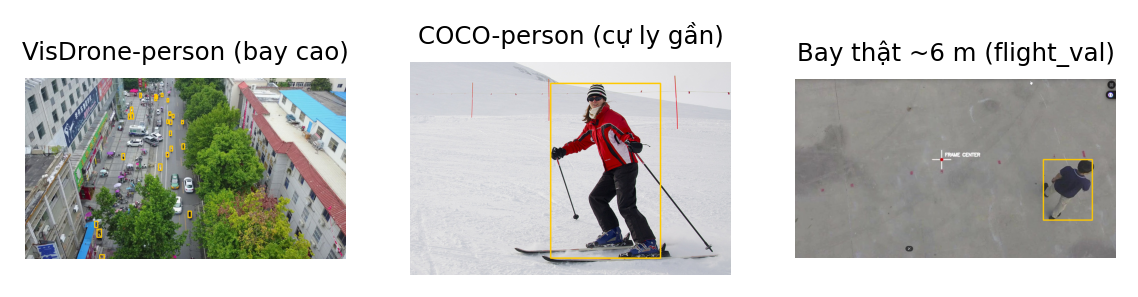
\includegraphics[width=\textwidth]{mau_du_lieu.png}
\caption{Ba nguồn dữ liệu của đề tài và nhãn bounding box tương ứng: VisDrone-person chụp từ trên cao (trái), COCO-person ở cự ly gần (giữa) và khung hình bay thật ở độ cao khoảng 6\,m (phải)}
\label{fig:maudulieu}
\end{figure}

\section{Các bộ dữ liệu}

\subsection{VisDrone-person}

VisDrone2019-DET~\cite{zhu2022visdrone} là bộ dữ liệu phát hiện đối tượng từ UAV do Đại học Thiên Tân (Trung Quốc) công bố, chụp ở nhiều thành phố, độ cao và điều kiện ánh sáng, gồm mười lớp đối tượng. Đề tài chuyển bộ dữ liệu về bài toán một lớp bằng cách gộp hai lớp \texttt{pedestrian} (người đang đi hoặc đứng) và \texttt{people} (người ở tư thế khác như ngồi) thành lớp \textit{person}, vì hệ thống bám theo phải nhận ra người ở mọi tư thế. Các hộp có cạnh nhỏ hơn 10 điểm ảnh bị loại vì gần như không thể gán nhãn nhất quán. Nhãn được chuyển sang định dạng YOLO (tâm, rộng, cao chuẩn hoá về $[0,1]$). Kết quả gồm 6.471 ảnh huấn luyện với 65.523 hộp và 548 ảnh kiểm định với 8.165 hộp. Trong tập kiểm định, 98,7\% số hộp có diện tích dưới $32^2$ điểm ảnh sau khi đưa ảnh về $640\times640$, nên AP trên tập này gần như trùng với AP của vật nhỏ.

\subsection{COCO-person}

COCO~\cite{lin2014coco} chứa ảnh đời thường với người ở cự ly gần và nhiều tư thế. Đề tài lấy các chú thích lớp \textit{person} từ tập val2017, bỏ những hộp có diện tích dưới 100 điểm ảnh vuông, được 2.654 ảnh với 9.783 hộp. Tập này bổ sung cho mô hình kinh nghiệm về người kích thước lớn mà VisDrone gần như không có. Khi dùng, mỗi epoch trộn thêm một lượng ảnh COCO bằng 25\% số ảnh VisDrone (1.618 ảnh).

\subsection{Tập bay thật flight\_val}

Tập này được xây dựng từ chuyến bay thử ngày 21/07/2026 trên một bãi nền bê tông. Máy bay bay ở chế độ giữ vị trí, độ cao khoảng 6\,m, camera nhìn xuống, một người đi bộ bên dưới. Video được ghi từ màn hình trạm mặt đất, vùng giao diện được cắt bỏ, và một khung hình được lấy mỗi giây trong đoạn bay ổn định từ giây thứ 18 tới giây thứ 150. Nhãn được khởi tạo bằng mô hình rồi sửa tay từng khung trên công cụ Roboflow theo bộ quy tắc: hộp ôm sát toàn thân nhìn thấy, xoá mọi hộp sai (bóng, vết bẩn nền, biểu tượng giao diện), bổ sung người bị bỏ sót. Sau khi rà soát còn 92 khung hình $1174\times654$, mỗi khung có đúng một người. Tập này \textit{không} được dùng để huấn luyện, chọn mô hình hay hiệu chuẩn lượng tử hoá; nó chỉ dùng để đánh giá, nhằm tránh rò rỉ dữ liệu.

\begin{table}[H]
\centering
\caption{Thống kê ba bộ dữ liệu sau chuẩn hoá (lớp duy nhất \textit{person})}
\label{tab:dulieu}
\small
\renewcommand{\arraystretch}{1.15}
\begin{tabularx}{\textwidth}{@{}l>{\centering\arraybackslash}X>{\centering\arraybackslash}X>{\centering\arraybackslash}X>{\raggedright\arraybackslash}p{4.2cm}@{}}
\toprule
\textbf{Bộ dữ liệu} & \textbf{Số ảnh} & \textbf{Số hộp} & \textbf{Trung vị diện tích hộp @640 (px$^2$)} & \textbf{Vai trò}\\
\midrule
VisDrone-person huấn luyện & 6.471 & 65.523 & -- & Huấn luyện\\
VisDrone-person kiểm định & 548 & 8.165 & 122 & Chọn mô hình, so sánh, đánh giá rung\\
COCO-person & 2.654 & 9.783 & -- & Bổ sung người cự ly gần (nhánh triển khai)\\
flight\_val (bay thật $\approx$6\,m) & 92 & 92 & 7.874 & Chỉ đánh giá trên miền triển khai\\
\bottomrule
\end{tabularx}
\end{table}

\section{Hai nhánh mô hình}
\label{sec:hainhanh}

Để vừa so sánh công bằng với các công trình khác, vừa phục vụ triển khai thật, đề tài duy trì hai nhánh huấn luyện độc lập dùng chung một kiến trúc:
\begin{itemize}
\item \textbf{Nhánh chuẩn:} chỉ huấn luyện trên VisDrone-person, không thêm dữ liệu ngoài. Mọi bảng so sánh với mô hình đối chứng dùng nhánh này, để chênh lệch không đến từ dữ liệu bổ sung.
\item \textbf{Nhánh triển khai:} huấn luyện trên VisDrone-person trộn COCO-person, nhắm tới người ở cự ly gần. Mô hình chạy trên máy bay thuộc nhánh này.
\end{itemize}

\section{Tiền xử lý và data augmentation}

Ảnh được co giãn giữ nguyên tỷ lệ về cạnh dài 640 điểm ảnh và đệm phần thiếu bằng màu xám (letterbox), toạ độ nhãn được biến đổi tương ứng. Trong huấn luyện, đề tài dùng các phép tăng cường chuẩn: ghép bốn ảnh (xác suất 0,5, tắt ở các epoch cuối để mô hình quen với ảnh đơn), trộn hai ảnh (0,1), lật ngang (0,5), biến đổi affine, thay đổi màu, sao chép dán đối tượng (0,4), một số phép biến đổi đặc thù ảnh UAV (0,3), và huấn luyện đa tỷ lệ với kích thước ảnh ngẫu nhiên từ 50\% tới 100\% của 640, bước 32 điểm ảnh. Các phép này đều là những biến đổi mà dữ liệu gốc đã phần nào chứa đựng; không phép nào mô phỏng rung của khung máy bay. Suy giảm do rung được đưa vào riêng ở Chương~\ref{chap:mohinh}.

\section{Giao thức mô phỏng rung VisDrone-Shake}
\label{sec:shake}

\subsection{Mô hình suy giảm}

Giao thức hiện thực phương trình~(\ref{eq:rung}) trên ảnh đã chuẩn hoá về $[0,1]$ theo ba bước: (1) tích chập theo từng kênh màu với nhân nhoè dạng đoạn thẳng dài $L$ điểm ảnh, hướng $\theta$ lấy ngẫu nhiên đều trong $[0^\circ, 180^\circ)$, nhân được chuẩn hoá tổng bằng 1; (2) cộng nhiễu Gauss độ lệch chuẩn $\sigma$; (3) nhân toàn ảnh với hệ số $1+u$, $u$ lấy đều trong $[-b, b]$. Ba mức suy giảm được định nghĩa trong Bảng~\ref{tab:shake} và minh hoạ ở Hình~\ref{fig:rungminhhoa}. Mức 1 và mức 2 tương ứng máy bay cân bằng tốt đang bay ổn định hoặc bay tiến; mức 3 tương ứng kích thích mạnh như cánh quạt mất cân bằng.

\begin{table}[H]
\centering
\caption{Tham số ba mức rung của giao thức VisDrone-Shake}
\label{tab:shake}
\small
\renewcommand{\arraystretch}{1.15}
\begin{tabular}{@{}lcccl@{}}
\toprule
\textbf{Mức} & \textbf{Độ dài nhoè $L$ (px)} & \textbf{Nhiễu $\sigma$} & \textbf{Dao động sáng $b$} & \textbf{Tình huống tương ứng}\\
\midrule
Mức 1 & 5 & 0,02 & $\pm$10\% & Bay treo, khung cân bằng tốt\\
Mức 2 & 9 & 0,04 & $\pm$20\% & Bay tiến thông thường\\
Mức 3 & 15 & 0,06 & $\pm$30\% & Kích thích mạnh (cánh quạt lệch)\\
\bottomrule
\end{tabular}
\end{table}

\begin{figure}[H]
\centering
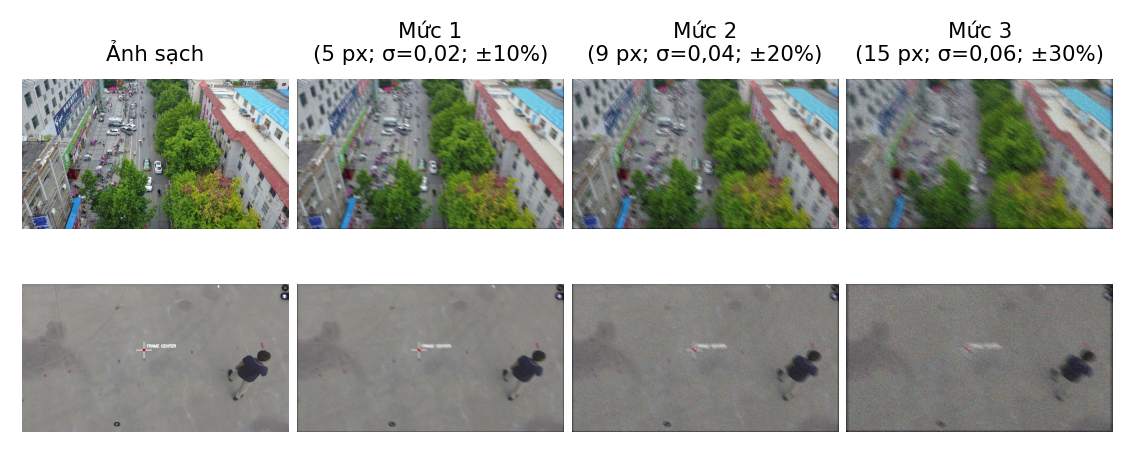
\includegraphics[width=\textwidth]{rung_minh_hoa.png}
\caption{Minh hoạ ba mức rung VisDrone-Shake trên một ảnh VisDrone (hàng trên) và một khung bay thật (hàng dưới); hướng nhoè cố định $35^\circ$ để dễ so sánh}
\label{fig:rungminhhoa}
\end{figure}

Điểm quan trọng là không bước nào trong ba bước làm dịch chuyển đối tượng: nhoè đối xứng quanh tâm, nhiễu và độ sáng không đổi hình học. Vì vậy bounding box gốc vẫn hợp lệ trên ảnh đã suy giảm, và cùng một toán tử có thể dùng cho cả đánh giá lẫn huấn luyện mà không phải sửa nhãn.

\subsection{Giao thức phải được cố định seed ngẫu nhiên}

Hướng nhoè, nhiễu và độ sáng đều được rút ngẫu nhiên, nên một lần chạy đánh giá chỉ là một lần rút thăm. Trong quá trình làm đề tài, nhóm đã đo cùng một checkpoint ba lần mà không cố định hạt giống và nhận được tỷ lệ retain 17,0\%, 17,1\% và 17,6\%, tức dao động hơn nửa điểm phần trăm, đủ để tạo ra một ``cải tiến'' giả. Giao thức chính thức vì thế gieo lại hạt giống trước \textit{mỗi} lượt đánh giá ở mỗi mức, chạy với ba hạt giống 0, 1, 2 và báo cáo trung bình $\pm$ độ lệch chuẩn mẫu. Đánh giá trên ảnh sạch là tất định nên chỉ chạy một lần. Chỉ số tổng hợp là mCP và retain theo phương trình~(\ref{eq:mcp}) với $M=3$.

\section{Một chương trình đo duy nhất cho mọi mô hình}
\label{sec:mottrinhdo}

Mỗi họ mô hình đi kèm chương trình đánh giá riêng với ngưỡng tin cậy, số hộp tối đa và quy ước diện tích khác nhau. Khi đo lại YOLOv8-n bằng chương trình của Ultralytics, nhóm được AP@[.50:.95] = 0,2787; khi đo bằng chương trình chung của đề tài, được 0,2684. Chênh lệch 0,01 này cùng cỡ với khoảng cách giữa các mô hình đối chứng với nhau, nên nếu trộn hai chương trình đo trong cùng một bảng, người đọc sẽ nhầm khác biệt do cách đo thành khác biệt giữa các mô hình. Với RT-DETR-l chênh lệch còn lớn hơn (0,3340 so với 0,2502), vì bộ tiền xử lý gốc của nó kéo giãn ảnh cho vuông thay vì đệm xám.

Do đó, \textbf{mọi mô hình trong mọi bảng của Chương~\ref{chap:ketqua}} được đo bằng một chương trình duy nhất (\texttt{paper\_eval\_unified.py}) với cùng cấu hình:
\begin{itemize}
\item cùng bộ nạp ảnh letterbox $640\times640$, mọi mô hình nhận đúng cùng một tensor đầu vào;
\item ngưỡng tin cậy 0,01, NMS với ngưỡng IoU 0,5, tối đa 300 hộp mỗi ảnh;
\item chấm điểm bằng thư viện \texttt{pycocotools} trên cùng một tệp nhãn chuẩn;
\item ba hạt giống cho mọi lượt đánh giá có rung.
\end{itemize}
Chỉ số retain không bị ảnh hưởng bởi cách tiền xử lý của từng mô hình vì nó là tỷ số giữa hai lượt đo trong cùng một đường xử lý; tuy vậy, đề tài vẫn ghi chú rõ trường hợp RT-DETR-l trong bảng kết quả.

\section{Quy tắc chọn checkpoint}

Mỗi lần huấn luyện sinh ra checkpoint tốt nhất theo AP kiểm định trên ảnh sạch (\texttt{best.pt}) và checkpoint cuối (\texttt{last.pt}). Với SteadyDet-W được huấn luyện có ràng buộc nhất quán, \texttt{last.pt} cho retain 33,4\% còn \texttt{best.pt} cho 30,5\%. Nếu lấy \texttt{last.pt} cho mô hình của mình và \texttt{best.pt} cho mô hình đối chứng thì đó là hai quy tắc khác nhau và kết quả bị thiên vị. Đề tài áp dụng một quy tắc duy nhất: \textbf{mọi mô hình dùng checkpoint tốt nhất theo AP sạch}, không checkpoint nào được chọn dựa trên chính giao thức rung dùng để đánh giá nó.

\section{Đánh giá trên miền triển khai}

Trên tập flight\_val, các mô hình được đánh giá bằng hai cách bổ trợ. Cách thứ nhất dùng cùng hàm \texttt{pycocotools} để tính AP@0,5, AP@[.50:.95], AP@0,75 và AR@100. Vì chỉ có 92 khung, đề tài lấy mẫu lại khung hình 1.000 lần theo phương pháp bootstrap ghép cặp để tính khoảng tin cậy 95\% cho hiệu giữa hai mô hình. Cách thứ hai sát với vận hành hơn: chạy mô hình một lần ở ngưỡng tin cậy thấp 0,02 rồi quét ngưỡng ngoại tuyến, tại mỗi ngưỡng ghép dự đoán với nhãn bằng IoU $\ge 0{,}5$ để tính precision, recall, F1 và số hộp sai mỗi khung. Ngưỡng cho F1 cao nhất được chọn làm ngưỡng vận hành trên máy bay.

Khi so sánh mô hình FP32 và INT8, cả hai được xuất dự đoán ra cùng một định dạng và chấm bằng cùng một hàm, để chênh lệch chỉ phản ánh tác động của lượng tử hoá.

\section{Môi trường thực nghiệm}

\begin{table}[H]
\centering
\caption{Môi trường phần cứng và phần mềm dùng trong đề tài}
\label{tab:moitruong}
\small
\renewcommand{\arraystretch}{1.15}
\begin{tabularx}{\textwidth}{@{}l>{\raggedright\arraybackslash}X@{}}
\toprule
\textbf{Hạng mục} & \textbf{Cấu hình}\\
\midrule
Máy huấn luyện & Máy tính xách tay GPU NVIDIA RTX 4060 Laptop 8\,GB, RAM 14\,GB, CUDA; PyTorch; Ultralytics 8.4 cho các mô hình đối chứng\\
Máy tính trên UAV & Raspberry Pi~5 (Debian 12, nhân 6.12, aarch64), Python 3.11\\
Bộ tăng tốc & Hailo-8L qua PCIe, HailoRT 4.20.0; biên dịch bằng Hailo Dataflow Compiler 3.34 trên máy x86\\
Camera & Logitech C270 HD, USB, MJPG, tối đa $1280\times720$ ở 30 khung hình/giây\\
Bộ điều khiển bay & Holybro Pixhawk~6C, ArduPilot Copter 4.7.0, kết nối USB, MAVLink v2\\
Phần mềm hỗ trợ & Mission Planner (cấu hình tham số), pymavlink, OpenCV, NumPy, SciPy\\
\bottomrule
\end{tabularx}
\end{table}

\section{Kết luận chương}

Đề tài sử dụng ba nguồn dữ liệu bao phủ hai miền: VisDrone-person cho so sánh chuẩn, COCO-person bổ sung người cự ly gần, và 92 khung bay thật chỉ dùng để đánh giá trên miền triển khai. Giao thức VisDrone-Shake mô phỏng ba hiệu ứng vật lý của rung mà không làm sai nhãn, được cố định seed và lặp ba lần. Mọi mô hình được đo bằng một chương trình duy nhất và chọn checkpoint theo một quy tắc duy nhất. Những ràng buộc này đảm bảo các so sánh ở Chương~\ref{chap:ketqua} phản ánh khác biệt thật giữa các mô hình.

% =====================================================================
%  CHƯƠNG 3. MÔ HÌNH STEADYDET-N VÀ HUẤN LUYỆN NHẬN BIẾT RUNG
% =====================================================================
\chapter{Mô hình SteadyDet-N và phương pháp huấn luyện nhận biết rung}
\label{chap:mohinh}

Chương này trình bày mô hình phát hiện người do đề tài xây dựng. Phần đầu mô tả quá trình đi tới kiến trúc cuối cùng và lý do của từng lựa chọn; phần sau trình bày hàm mất mát, quy trình huấn luyện và phương pháp huấn luyện nhận biết rung, là đóng góp chính về mặt mô hình của đề tài.

\section{Yêu cầu thiết kế}

Mô hình phải thoả mãn đồng thời bốn yêu cầu, mỗi yêu cầu xuất phát từ một ràng buộc cụ thể của hệ thống:
\begin{enumerate}
\item \textbf{Phát hiện được người nhỏ}: khi máy bay lên cao hoặc người đi xa, bounding box chỉ còn vài chục điểm ảnh vuông, nên mô hình cần một mức dự đoán độ phân giải cao.
\item \textbf{Chi phí tính toán thấp}: một khung hình phải đi qua camera, mô hình, bộ theo vết và bộ điều khiển trong ngân sách 33,3\,ms của vòng lặp 30\,Hz trên một máy tính nhúng tản nhiệt thụ động.
\item \textbf{Chỉ dùng các phép toán mà NPU hỗ trợ}: mô hình phải biên dịch được bằng Hailo DFC và lượng tử hoá INT8 được.
\item \textbf{Bền trước rung}: độ chính xác phải giữ được khi ảnh bị nhoè và nhiễu do rung của khung máy bay.
\end{enumerate}

\section{Quá trình phát triển kiến trúc}

Kiến trúc được phát triển qua nhiều phiên bản, mỗi phiên bản được đo đạc trước khi quyết định hướng tiếp theo. Hai phiên bản quan trọng nhất được đặt tên trong báo cáo là \textbf{SteadyDet-W} (bản rộng) và \textbf{SteadyDet-N} (bản nano, bản cuối cùng). Trong mã nguồn, hai mô hình này tương ứng các tệp \texttt{pfdet\_nano\_v15.py} và \texttt{pfdet\_nano\_v17.py}.

SteadyDet-W đã có ít tham số (1,00 triệu) và chính xác nhất trong các phiên bản của nhóm, nhưng chi phí tính toán tới 12,9 GFLOPs ở độ phân giải 640. Phân tích chi phí theo từng lớp cho thấy nguyên nhân: riêng head ở mức $P_2$ ($160\times160$) đã tiêu tốn 1,82 GMACs, tức 28\% tổng chi phí, vì nó dùng năm lớp tích chập đầy đủ trên bản đồ lớn nhất. Đây là minh hoạ trực tiếp cho nhận xét ở Chương~\ref{chap:lythuyet}: số tham số ít không đồng nghĩa với chạy nhanh, vì chi phí tỷ lệ với diện tích feature map mà lớp đó xử lý. SteadyDet-N ra đời để giữ mức $P_2$ nhưng làm cho nó rẻ.

\section{Kiến trúc SteadyDet-N}
\label{sec:kientruc}

Hình~\ref{fig:kientruc} mô tả kiến trúc SteadyDet-N với cấu hình \textit{light} dùng trong toàn bộ đề tài. Mô hình có 1,17 triệu tham số và 4,6 GFLOPs với ảnh vào $640\times640$, là mô hình nhỏ nhất và rẻ nhất trong mọi bảng so sánh của báo cáo.

\begin{figure}[H]
\centering
\resizebox{0.97\textwidth}{!}{% Sơ đồ kiến trúc SteadyDet-N (profile light, ảnh vào 640x640)
\begin{tikzpicture}[
  font=\footnotesize, >={Stealth[length=2mm]},
  blk/.style={draw=black!60, rounded corners=2pt, align=center, minimum height=8.5mm, inner sep=2pt, fill=white},
  bb/.style={blk, fill=black!6, minimum width=3.3cm},
  nk/.style={blk, fill=xanh!10, minimum width=2.2cm},
  hd/.style={blk, fill=cam!12, minimum width=2.4cm},
  p2/.style={dashed, thick},
  lab/.style={font=\scriptsize, text=black!65}
]
% backbone
\node[blk, minimum width=3.3cm, fill=black!2] (in) at (0,0) {Ảnh vào\\$640\times640\times3$};
\node[bb, below=4mm of in] (stem) {EdgeContextStem\\$P_1$: $320^2$, 24 kênh};
\node[bb, below=4mm of stem, p2] (s2) {UIB (1 khối, bước 2)\\$P_2$: $160^2$, 48 kênh};
\node[bb, below=4mm of s2] (s3) {CSP-UIB (2 khối)\\$P_3$: $80^2$, 96 kênh};
\node[bb, below=4mm of s3] (s4) {CSP-UIB (2 khối)\\$P_4$: $40^2$, 144 kênh};
\node[bb, below=4mm of s4] (s5) {CSP-UIB (2 khối)\\$P_5$: $20^2$, 192 kênh};
\node[bb, below=4mm of s5, fill=xanh!22] (att) {Window self-attention\\(chỉ ở $P_5$)};
\foreach \a/\b in {in/stem,stem/s2,s2/s3,s3/s4,s4/s5,s5/att} \draw[->] (\a) -- (\b);

% neck (top-down)
\node[nk, right=2.3cm of att] (n5) {Conv $1\times1$\\48 kênh};
\node[nk, above=9.5mm of n5] (n4) {UIB\\48 kênh};
\node[nk, above=9.5mm of n4] (n3) {UIB\\48 kênh};
\node[nk, above=9.5mm of n3, p2] (n2) {UIB\\24 kênh};
\draw[->] (att) -- node[lab,above]{chiếu $1\times1$} (n5);
\draw[->] (s4.east) -- ++(0.9,0) |- (n4.west);
\draw[->] (s3.east) -- ++(0.7,0) |- (n3.west);
\draw[->] (s2.east) -- ++(0.5,0) |- (n2.west);
\draw[->, xanh, thick] (n5) -- node[lab,right]{$\uparrow2$, cộng} (n4);
\draw[->, xanh, thick] (n4) -- node[lab,right]{$\uparrow2$, cộng} (n3);
\draw[->, xanh, thick] (n3) -- node[lab,right]{$1\times1$, $\uparrow2$, cộng} (n2);

% heads
\node[hd, right=1.9cm of n2, p2] (h2) {LiteHead\\ra $160^2\times5$};
\node[hd, right=1.9cm of n3] (h3) {LiteHead\\ra $80^2\times5$};
\node[hd, right=1.9cm of n4] (h4) {LiteHead\\ra $40^2\times5$};
\node[hd, right=1.9cm of n5] (h5) {LiteHead\\ra $20^2\times5$};
\foreach \a/\b in {n2/h2,n3/h3,n4/h4,n5/h5} \draw[->] (\a) -- (\b);

\node[lab, above=1mm of s2.north east, anchor=south west, xshift=-4mm] {};
\node[font=\footnotesize\bfseries] at (0,1.0) {Backbone};
\node[font=\footnotesize\bfseries] at (n2 |- 0,1.0) {FPN neck (từ trên xuống)};
\node[font=\footnotesize\bfseries] at (h2 |- 0,1.0) {Head};
\node[draw=black!40, rounded corners=2pt, fill=black!3, align=left, font=\scriptsize, text width=3.9cm, below=6mm of h5] (lh)
 {\textbf{LiteHead:} DW $3\times3$ + PW $1\times1$ dùng chung $\rightarrow$ 1 kênh điểm người + 4 kênh hộp (hồi quy trực tiếp, không DFL).\\[2pt]
  Nét đứt: nhánh $P_2$ bước 4 được làm mỏng (1 khối, nửa số kênh neck, head depthwise separable).};
\end{tikzpicture}
}
\caption{Kiến trúc SteadyDet-N; độ phân giải giảm dần từ trên xuống. Chi phí được phân bổ không đối xứng: nhánh $P_2$ (nét đứt) chỉ có một khối, số kênh bằng một nửa và head tách được, còn các khối CSP hai tầng và phép self-attention nằm ở những mức có bản đồ nhỏ}
\label{fig:kientruc}
\end{figure}

\subsection{Backbone}

\textbf{Khối đầu vào EdgeContextStem.} Ảnh vào được xử lý song song bởi hai nhánh: nhánh cục bộ gồm hai tích chập $3\times3$ (lớp đầu có bước 2) giữ chi tiết cạnh, và nhánh ngữ cảnh gồm phép lấy trung bình $2\times2$ rồi một tích chập $3\times3$. Hai nhánh được ghép kênh và trộn bằng tích chập $1\times1$, cho ra bản đồ $P_1$ kích thước $320\times320$ với 24 kênh. Việc giảm độ phân giải bằng hai con đường bổ trợ giúp giữ thông tin của các vật rất nhỏ ngay từ lớp đầu tiên.

\textbf{Mức $P_2$ chỉ một khối.} Mức bước 4 dùng đúng một khối UIB~\cite{qin2024mnv4} có bước 2, gồm tích chập depthwise $3\times3$, mở rộng kênh $1\times1$ với hệ số 4, rồi thu hẹp $1\times1$ về 48 kênh. SteadyDet-W dùng ba khối ở mức này; giảm xuống một khối cắt phần lớn chi phí của mức đắt nhất.

\textbf{Các mức $P_3$--$P_5$.} Ba mức sâu hơn dùng khối CSP-UIB: một khối UIB giảm mẫu, sau đó bản đồ được tách thành hai nửa theo kênh, một nửa đi qua hai khối UIB, nửa kia đi tắt, rồi hai nửa được ghép lại và trộn bằng tích chập $1\times1$ theo ý tưởng của CSPNet~\cite{wang2020cspnet}. Số kênh lần lượt là 96, 144 và 192. Ở $P_3$ và $P_4$, khối UIB có thêm một tích chập depthwise để mở rộng receptive field với chi phí thấp. Chi phí tính toán được dồn vào các mức này vì bản đồ ở đây nhỏ: $80\times80$, $40\times40$ và $20\times20$.

\textbf{Self-attention chỉ ở $P_5$.} Sau mức $P_5$, một khối self-attention theo cửa sổ~\cite{liu2021swin} với window size 3 và 2 attention head cho mô hình ngữ cảnh toàn cục (ví dụ phân biệt người với cột điện hay bóng đổ). Đặt ở $20\times20$ nên chi phí của nó không đáng kể.

\subsection{FPN neck mỏng}

Neck của mạng là một FPN~\cite{lin2017fpn} chỉ có đường từ trên xuống. Mỗi mức của backbone được chiếu về số kênh chung bằng tích chập $1\times1$: 48 kênh cho $P_3$--$P_5$ và chỉ \textbf{24 kênh cho $P_2$}. Bản đồ mức trên được phóng to gấp đôi bằng nội suy nearest-neighbor, cộng với bản đồ mức dưới, rồi đi qua một khối UIB. Riêng khi đi từ $P_3$ xuống $P_2$, bản đồ được chiếu từ 48 về 24 kênh trước khi phóng to. Việc giảm một nửa số kênh ở mức $160\times160$ làm chi phí mọi lớp ở mức này giảm khoảng bốn lần.

\subsection{Head LiteHead}

Mỗi mức có một head LiteHead gồm một tích chập depthwise $3\times3$ và một tích chập $1\times1$ dùng chung, sau đó tách thành hai tích chập $1\times1$: một cho điểm có người (1 kênh), một cho bounding box (4 kênh). Như vậy mỗi head xuất một tensor $5 \times H \times W$ ở bốn bước 4, 8, 16 và 32. So với head tách rời năm lớp tích chập đầy đủ của SteadyDet-W, LiteHead rẻ hơn nhiều mà vẫn tách hai nhiệm vụ phân loại và hồi quy. Hộp được hồi quy trực tiếp (không dùng phân phối rời rạc), tương tự hướng của YOLO26~\cite{ultralytics}. Độ lệch ban đầu của kênh phân loại được đặt bằng $-5{,}5$ để xác suất ban đầu xấp xỉ 0,004, tránh việc hàng chục nghìn ô nền sinh hộp sai trong những epoch đầu.

\textbf{Giải mã.} Với grid cell $(i, j)$ ở bước $s$ và đầu ra $(t_x, t_y, t_w, t_h)$, hộp dự đoán được giải mã như sau:
\begin{equation}
c_x = \big(j + \mathrm{sigmoid}(t_x) - 0{,}5\big)\, s, \quad
c_y = \big(i + \mathrm{sigmoid}(t_y) - 0{,}5\big)\, s, \quad
w = e^{t_w} s, \quad h = e^{t_h} s.
\label{eq:decode}
\end{equation}
Mọi phép toán của mô hình (tích chập, batch norm được gộp vào tích chập, SiLU, cộng, ghép kênh, nội suy) đều được Hailo DFC hỗ trợ, trừ khối self-attention; Chương~\ref{chap:trienkhai} trình bày cách xử lý khối này khi triển khai.

\subsection{So sánh hai phiên bản}

\begin{table}[H]
\centering
\caption{So sánh cấu trúc và chi phí của SteadyDet-W và SteadyDet-N (ảnh vào $640\times640$)}
\label{tab:sosanhkientruc}
\small
\renewcommand{\arraystretch}{1.15}
\begin{tabularx}{\textwidth}{@{}l>{\centering\arraybackslash}X>{\centering\arraybackslash}X@{}}
\toprule
\textbf{Thành phần} & \textbf{SteadyDet-W} & \textbf{SteadyDet-N}\\
\midrule
Số khối ở mức $P_2$ & 3 & 1\\
Số kênh cổ ở mức $P_2$ & bằng các mức khác & một nửa (24)\\
Head & tách rời 5 tích chập đầy đủ & LiteHead depthwise separable\\
Vị trí self-attention & $P_4$ và $P_5$ & chỉ $P_5$\\
Số tham số & 1,00 triệu & 1,17 triệu\\
Chi phí tính toán & 12,9 GFLOPs & \textbf{4,6 GFLOPs} (giảm 2,8 lần)\\
\bottomrule
\end{tabularx}
\end{table}

SteadyDet-N có nhiều tham số hơn SteadyDet-W một chút vì phần tính toán được dồn về các mức sâu, nơi số kênh lớn; nhưng chính các mức này có bản đồ nhỏ nên tổng chi phí giảm 2,8 lần.

\section{Hàm mất mát}
\label{sec:hammatmat}

Tổng hàm mất mát gồm hai thành phần:
\begin{equation}
\mathcal{L}_{\det} = \lambda_{\text{obj}}(e)\, \mathcal{L}_{\text{obj}} + \lambda_{\text{box}}(e)\, \mathcal{L}_{\text{box}},
\end{equation}
trong đó $e$ là chỉ số epoch.

\textbf{Thành phần phân loại} $\mathcal{L}_{\text{obj}}$ là hàm QFL~\cite{li2020gfl} theo phương trình~(\ref{eq:qfl}) với $\beta = 2$, nhãn mềm là IoU giữa hộp dự đoán và hộp thật tại các ô dương.

\textbf{Thành phần hồi quy} kết hợp NWD và CIoU với trọng số phụ thuộc diện tích hộp thật $A$ (điểm ảnh vuông):
\begin{equation}
\mathcal{L}_{\text{box}} = w_{\text{ASL}}(A)\Big[\, \omega(A)\,\big(1 - \mathrm{NWD}\big) + \big(1 - \omega(A)\big)\,\mathcal{L}_{\mathrm{CIoU}} \Big],
\qquad \omega(A) = \exp\!\left(-\frac{A}{1024}\right).
\label{eq:boxloss}
\end{equation}
Với người rất nhỏ ($A \ll 32^2$), $\omega \approx 1$ và NWD chiếm ưu thế nhờ gradient ổn định; với người lớn, CIoU chiếm ưu thế vì nó phạt chính xác hình dạng hộp. Hằng số chuẩn hoá NWD là $C = 0{,}019$ theo toạ độ chuẩn hoá. Hệ số $w_{\text{ASL}}(A) = \mathrm{clip}\big(\sqrt{A_{\text{ref}}/A},\, 1,\, 4\big)$ tăng trọng số cho vật nhỏ, với $A_{\text{ref}}$ tương ứng 0,4\% diện tích ảnh.

\textbf{Gán nhãn nhận biết mục tiêu nhỏ.} Việc chọn ô dương dựa trên mức độ phù hợp theo TOOD~\cite{feng2021tood}, $t = s^{\alpha}\cdot \mathrm{IoU}^{\beta}$ với $\alpha = 1$, $\beta = 8$. Vì một người nhỏ chỉ phủ vài grid cell, chiến lược mặc định dễ cấp cho họ quá ít ô dương. Đề tài áp dụng hai điều chỉnh: người có diện tích dưới 576 điểm ảnh vuông ($24^2$) được cấp tới 6 ô dương và vùng tìm kiếm bán kính 3 ô, còn người lớn hơn được cấp 3 ô với bán kính 2; đồng thời số ô dương tối thiểu cho mục tiêu nhỏ không dưới 4.

\textbf{Cân bằng tiến triển.} Ở đầu quá trình huấn luyện, mô hình cần học ``có người hay không'' trước khi học ``hộp khít tới đâu''. Trọng số hai thành phần được nội suy tuyến tính theo tiến độ huấn luyện: $\lambda_{\text{obj}}$ giảm từ $2\times8$ về 8 và $\lambda_{\text{box}}$ tăng từ $4/2$ lên 4.

\section{Quy trình huấn luyện}
\label{sec:quytrinhhuanluyen}

\textbf{Bộ tối ưu.} Đề tài dùng MuSGD, bộ tối ưu lai được Ultralytics giới thiệu cùng YOLO26~\cite{ultralytics}, kết hợp Muon~\cite{jordan2024muon} với SGD có quán tính Nesterov. Với các tensor trọng số nhiều chiều, bước cập nhật là tổng của hai phần: phần Muon (hệ số 0,2), trong đó gradient được trực giao hoá xấp xỉ bằng 5 vòng lặp Newton--Schulz, và phần SGD (hệ số 1,0); các tham số một chiều (độ lệch, batch norm) chỉ dùng SGD. Trong các thử nghiệm của nhóm trên SteadyDet-W, MuSGD cho AP@0,5 kiểm định 0,5932, cao nhất trong các bộ tối ưu đã thử.

\textbf{Huấn luyện gốc (nhánh chuẩn).} SteadyDet-N được huấn luyện từ khởi tạo ngẫu nhiên trong 300 epoch, batch size 16 với tích luỹ gradient 6 bước, learning rate 0,01 giảm theo hàm cosin xuống $10^{-4}$, 10 epoch warm-up, weight decay $5\times10^{-4}$, huấn luyện độ chính xác hỗn hợp và EMA của trọng số với hệ số 0,9998. Phép ghép bốn ảnh được tắt trong 60 epoch cuối. Mô hình được đánh giá trên tập kiểm định sau mỗi 5 epoch.

\textbf{Nhánh triển khai.} Mô hình được huấn luyện 400 epoch với batch size 12; dữ liệu COCO-person được trộn với tỷ lệ 25\% từ epoch 100 tới epoch 360. Khi cần triển khai lên NPU, mô hình này được tinh chỉnh thêm 20 epoch với learning rate $10^{-3}$ ở cấu hình không có khối self-attention (Chương~\ref{chap:trienkhai}).

\begin{figure}[H]
\centering
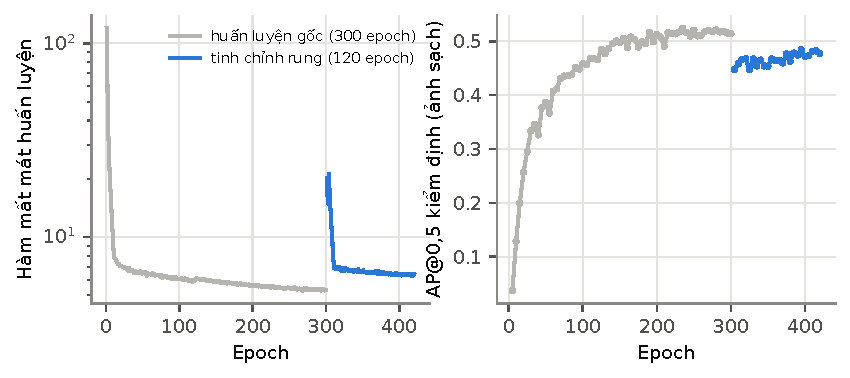
\includegraphics[width=\textwidth]{huan_luyen.pdf}
\caption{Hàm mất mát huấn luyện (trái, thang log) và AP@0,5 trên tập kiểm định ảnh sạch (phải) của SteadyDet-N nhánh chuẩn: 300 epoch huấn luyện gốc (xám) và 120 epoch tinh chỉnh nhận biết rung (xanh). Hàm mất mát tăng vọt khi bắt đầu tinh chỉnh vì một nửa số lô là ảnh đã bị làm rung}
\label{fig:huanluyen}
\end{figure}

\section{Huấn luyện nhận biết rung}
\label{sec:huanluyenrung}

\subsection{Ý tưởng}

Nguyên nhân gốc khiến bộ phát hiện sụp đổ khi rung là \textit{sai lệch phân phối}: VisDrone được thu từ các nền tảng ổn định, nên mô hình chưa bao giờ thấy ảnh nhoè do rung trong huấn luyện nhưng lại gặp nó liên tục khi bay. Các phép tăng cường chuẩn ở Chương~\ref{chap:dulieu} như lật ảnh, co giãn hay đổi màu chỉ lấy mẫu những biến đổi mà dữ liệu vốn đã chứa; chúng không sinh ra loại suy giảm này. Phương pháp của đề tài vì thế rất trực tiếp: đưa chính toán tử rung vào phân phối huấn luyện.

\subsection{Phương pháp}

Gọi $\mathcal{T}$ là toán tử rung ngẫu nhiên của giao thức VisDrone-Shake (mục~\ref{sec:shake}), trong đó mức rung được chọn ngẫu nhiên đều trong $\{1, 2, 3\}$ và hướng nhoè được rút lại cho mỗi batch. Trong huấn luyện, mỗi batch $x$ được thay bằng $\mathcal{T}(x)$ với xác suất $p = 0{,}5$, và hàm mất mát phát hiện thông thường được tính trên ảnh mà mạng nhận được:
\begin{equation}
\mathcal{L} = \mathcal{L}_{\det}\big(f_\theta(\hat{x}),\, y\big), \qquad
\hat{x} =
\begin{cases}
\mathcal{T}(x) & \text{với xác suất } p,\\
x & \text{ngược lại}.
\end{cases}
\label{eq:vibaware}
\end{equation}
Vì $\mathcal{T}$ không làm dịch chuyển đối tượng, nhãn $y$ không cần điều chỉnh; đây chính là điều làm cho phép thay thế hợp lệ. Phương pháp không thêm mô-đun nào, không cần truyền xuôi hai lần, và mô hình xuất ra để triển khai có cấu trúc giống hệt mô hình gốc, nên \textbf{chi phí suy luận không thay đổi}. Chi phí huấn luyện tăng thêm chỉ là một phép tích chập depthwise và hai phép toán từng phần tử trên GPU. Hình~\ref{fig:huanluyenrung}(a) minh hoạ phương pháp.

\begin{figure}[H]
\centering
\resizebox{\textwidth}{!}{% Sơ đồ huấn luyện nhận biết rung (trên) và biến thể ràng buộc nhất quán (dưới)
\begin{tikzpicture}[
  font=\footnotesize, >={Stealth[length=2mm]},
  box/.style={draw=black!60, rounded corners=2pt, align=center, minimum height=9mm, inner sep=3pt, fill=white},
  op/.style={box, fill=cam!14},
  net/.style={box, fill=xanh!14, minimum width=2.1cm},
  loss/.style={box, fill=black!7},
  dec/.style={diamond, draw=black!60, aspect=2.2, inner sep=1pt, align=center, fill=white, font=\scriptsize}
]
\node[font=\footnotesize\bfseries, anchor=west] at (-0.4,1.1) {(a) Huấn luyện nhận biết rung (phương pháp đề xuất)};
\node[box] (x) at (0,0) {Lô ảnh $x$\\+ nhãn $y$};
\node[dec, right=6mm of x] (d) {xác suất\\$p=0{,}5$};
\node[op, right=7mm of d] (T) {Toán tử rung $\mathcal{T}$\\nhoè $L,\theta$ + nhiễu $\sigma$ + sáng $b$};
\node[net, right=7mm of T] (f) {Mạng\\$f_\theta$};
\node[loss, right=7mm of f] (L) {$\mathcal{L}_{\det}\big(f_\theta(\hat{x}), y\big)$\\nhãn giữ nguyên};
\draw[->] (x) -- (d);
\draw[->] (d) -- node[above,font=\scriptsize]{có} (T);
\draw[->] (T) -- node[above,font=\scriptsize]{$\hat x$} (f);
\draw[->] (d.south) -- ++(0,-0.55) -| node[pos=0.25,below,font=\scriptsize]{không: $\hat x = x$} (f.south);
\draw[->] (f) -- (L);

\begin{scope}[yshift=-3.75cm]
\node[font=\footnotesize\bfseries, anchor=west] at (-0.4,1.5) {(b) Biến thể ràng buộc nhất quán (đối chứng, cho kết quả kém hơn)};
\node[box] (x2) at (0,0) {Lô ảnh $x$\\+ nhãn $y$};
\node[net] (fc) at (4.2,0.75) {$f_\theta(x)$ nhánh sạch};
\node[op] (T2) at (2.0,-0.75) {$\mathcal{T}$};
\node[net] (fv) at (4.2,-0.75) {$f_\theta(\tilde x)$ nhánh rung};
\node[loss, anchor=west] (Ld) at (7.4,0.75) {$\mathcal{L}_{\det}(f_\theta(x), y)$};
\node[loss, anchor=west] (sg) at (7.4,-0.75) {$\lambda\,\mathcal{L}_{\text{cons}}\big(f_\theta(\tilde x),\ \mathrm{sg}[f_\theta(x)]\big)$};
\draw[->] (x2.east) -- ++(0.35,0) |- (fc.west);
\draw[->] (x2.east) -- ++(0.35,0) |- (T2.west);
\draw[->] (T2) -- node[above,font=\scriptsize]{$\tilde x$} (fv);
\draw[->] (fc) -- (Ld);
\draw[->] (fv) -- (sg);
\draw[->, dashed] (fc.east) ++(0.2,0) -- node[left,font=\scriptsize, pos=0.5]{dừng gradient} ($(sg.north west)+(0.4,0)$);
\end{scope}
\end{tikzpicture}
}
\caption{(a) Huấn luyện nhận biết rung: một nửa số lô được thay bằng bản đã làm rung và tính hàm mất mát phát hiện thông thường. (b) Biến thể ràng buộc nhất quán: truyền xuôi cả hai bản và kéo dự đoán trên ảnh rung về phía dự đoán trên ảnh sạch đã dừng gradient. Cả hai chỉ tồn tại khi huấn luyện}
\label{fig:huanluyenrung}
\end{figure}

\subsection{Biến thể ràng buộc nhất quán}

Trước khi có kết quả, nhóm kỳ vọng rằng có thể khai thác nhiều tín hiệu hơn từ ảnh rung so với chỉ dùng nhãn. Biến thể này, lấy cảm hứng từ các phương pháp học bán giám sát dựa trên tính nhất quán, truyền cả $x$ và $\tilde{x} = \mathcal{T}(x)$ qua cùng một mạng, tính hàm mất mát phát hiện trên nhánh sạch, và thêm một thành phần kéo dự đoán trên ảnh rung về phía bản sao đã dừng gradient của dự đoán sạch:
\begin{equation}
\mathcal{L} = \mathcal{L}_{\det}\big(f_\theta(x), y\big) + \lambda\, \mathcal{L}_{\text{cons}}\Big(f_\theta(\tilde{x}),\ \mathrm{sg}\big[f_\theta(x)\big]\Big), \qquad \lambda = 0{,}5.
\label{eq:vibcons}
\end{equation}
$\mathcal{L}_{\text{cons}}$ gồm ba phần cộng trên các mức: entropy chéo có nhiệt độ $T = 2$ giữa điểm tin cậy hai nhánh, sai số $L_1$ trơn trên toạ độ hộp chỉ tại các ô mà nhánh sạch tin cậy trên 0,1, và sai số bình phương giữa đặc trưng cổ mạng với trọng số 0,5. Phép dừng gradient là bắt buộc: nếu thiếu nó, cách dễ nhất để giảm $\mathcal{L}_{\text{cons}}$ là làm dự đoán sạch kém đi cho giống dự đoán rung, tức phá huỷ bộ phát hiện. Biến thể này cần hai lượt truyền xuôi nên tốn khoảng 1,8 lần thời gian huấn luyện. Chương~\ref{chap:ketqua} cho thấy nó thực tế kém hơn phương pháp đơn giản.

\subsection{Thiết lập tinh chỉnh}

Huấn luyện nhận biết rung được áp dụng như một giai đoạn \textit{tinh chỉnh}: xuất phát từ checkpoint tốt nhất của huấn luyện gốc, tinh chỉnh 120 epoch với batch size 8 và tích luỹ gradient 12 bước, MuSGD với learning rate $2\times10^{-3}$, 3 epoch warm-up trước khi bật toán tử rung. Nhờ vậy phương pháp có thể áp dụng cho một mô hình đã huấn luyện xong mà không phải lặp lại toàn bộ lịch trình. Checkpoint được chọn theo AP kiểm định trên ảnh sạch, đúng quy tắc áp dụng cho mô hình gốc.

Để tách bạch tác dụng của rung khỏi tác dụng của việc huấn luyện thêm 120 epoch, đề tài chạy một \textbf{thí nghiệm đối chứng}: tinh chỉnh mô hình gốc đúng 120 epoch với cùng mọi siêu tham số nhưng tắt toán tử rung. Cả ba cấu hình (đối chứng, nhận biết rung, ràng buộc nhất quán) chỉ khác nhau đúng một biến.

\subsection{Biến thể không dùng NMS}

Đề tài cũng thử một biến thể SteadyDet-N không cần NMS theo ý tưởng của YOLOv10~\cite{wang2024yolov10}: thêm một head LiteHead ``one-to-one'' song song dùng chung đặc trưng, huấn luyện đồng thời với head ``one-to-many'', và khi suy luận chỉ dùng head one-to-one. Biến thể này đạt AP@[.50:.95] 0,1954 trên ảnh sạch và retain 23,4 $\pm$ 0,8\%. Tuy nhiên, trên hệ thống thực tế NMS chỉ tốn trung vị 0,84\,ms mỗi khung (Chương~\ref{chap:trienkhai}), nên việc bỏ NMS không mang lại lợi ích đáng kể về độ trễ; đề tài giữ head thông thường cho các thí nghiệm chính và triển khai.

\section{Kết luận chương}

SteadyDet-N giữ mức dự đoán bước 4 cho người nhỏ nhưng làm nhánh này mỏng đi, dồn tính toán về các mức sâu, dùng head depthwise separable, nhờ đó giảm chi phí 2,8 lần so với SteadyDet-W xuống 4,6 GFLOPs với 1,17 triệu tham số. Hàm mất mát kết hợp QFL, NWD và CIoU theo diện tích cùng chiến lược gán nhãn ưu tiên mục tiêu nhỏ. Phương pháp huấn luyện nhận biết rung đưa mô hình vật lý của rung vào phân phối huấn luyện, không đổi nhãn, không đổi mô hình khi suy luận. Chương tiếp theo kiểm chứng các thiết kế này bằng thực nghiệm có đối chứng.

% =====================================================================
%  CHƯƠNG 4. KẾT QUẢ THỰC NGHIỆM CỦA MÔ HÌNH
%  Nguồn số: runs/paper_queue/UNIFIED.json (1 chương trình đo, 3 seed),
%            runs/paper_queue/BASELINES_TABLE.md (tham số, GFLOPs),
%            runs/paper_queue/FLIGHT.json (92 khung bay thật, bootstrap).
% =====================================================================
\chapter{Kết quả thực nghiệm của mô hình}
\label{chap:ketqua}

Chương này trình bày kết quả đánh giá mô hình theo đúng giao thức ở Chương~\ref{chap:dulieu}. Mọi số liệu trên VisDrone-person được đo bằng một chương trình duy nhất; các cột có rung là trung bình $\pm$ độ lệch chuẩn qua ba hạt giống. Chương gồm bốn phần: tác dụng của huấn luyện nhận biết rung cùng các đối chứng; tính tổng quát và giới hạn của phương pháp; so sánh với năm mô hình nhẹ công khai; và kiểm chứng trên dữ liệu bay thật.

\section{Kết quả chính và các thí nghiệm đối chứng}
\label{sec:ketquachinh}

\begin{table}[H]
\centering
\caption{Kết quả trên VisDrone-person, ảnh $640\times640$. Trong mỗi khối, các dòng chỉ khác nhau đúng một yếu tố và dùng chung lịch trình, learning rate và phép tăng cường. Cột có rung: trung bình $\pm$ độ lệch chuẩn qua 3 hạt giống}
\label{tab:ketquachinh}
\footnotesize
\setlength{\tabcolsep}{3.2pt}
\renewcommand{\arraystretch}{1.18}
\resizebox{\textwidth}{!}{%
\begin{tabular}{@{}lccc|cccc@{}}
\toprule
 & \multicolumn{3}{c|}{\textbf{Ảnh sạch}} & \multicolumn{4}{c}{\textbf{Khi rung (AP@[.50:.95])}}\\
\textbf{Mô hình} & \textbf{AP} & \textbf{AP$_{50}$} & \textbf{AP$_{75}$} & \textbf{Mức 1} & \textbf{Mức 2} & \textbf{Mức 3} & \textbf{retain (\%)}\\
\midrule
\multicolumn{8}{@{}l}{\textit{SteadyDet-N (1,17 triệu tham số; 4,6 GFLOPs)}}\\
\quad Gốc & 0,1892 & 0,5127 & 0,0811 & \ms{0,0792}{0,0026} & \ms{0,0123}{0,0013} & \ms{0,0040}{0,0005} & \ms{16,8}{0,7}\\
\quad + 120 epoch không rung & 0,1823 & 0,4984 & 0,0762 & \ms{0,0761}{0,0028} & \ms{0,0125}{0,0005} & \ms{0,0040}{0,0005} & \ms{16,9}{0,7}\\
\quad + ràng buộc nhất quán & 0,1746 & 0,4837 & 0,0728 & \ms{0,1098}{0,0010} & \ms{0,0392}{0,0021} & \ms{0,0081}{0,0011} & \ms{30,0}{0,6}\\
\quad \textbf{+ huấn luyện nhận biết rung} & 0,1708 & 0,4731 & 0,0715 & \textbf{\ms{0,1223}{0,0014}} & \textbf{\ms{0,0518}{0,0019}} & \textbf{\ms{0,0111}{0,0002}} & \textbf{\ms{36,2}{0,7}}\\
\midrule
\multicolumn{8}{@{}l}{\textit{SteadyDet-W (1,00 triệu tham số; 12,9 GFLOPs)}}\\
\quad Gốc & 0,2349 & 0,5800 & 0,1305 & \ms{0,1260}{0,0023} & \ms{0,0258}{0,0022} & \ms{0,0046}{0,0026} & \ms{22,2}{0,9}\\
\quad + ràng buộc nhất quán & 0,2207 & 0,5561 & 0,1202 & \ms{0,1309}{0,0026} & \ms{0,0580}{0,0007} & \ms{0,0132}{0,0016} & \ms{30,5}{0,6}\\
\quad \textbf{+ huấn luyện nhận biết rung} & 0,2219 & 0,5511 & 0,1279 & \textbf{\ms{0,1583}{0,0013}} & \textbf{\ms{0,0839}{0,0001}} & \textbf{\ms{0,0200}{0,0012}} & \textbf{\ms{39,4}{0,3}}\\
\midrule
\multicolumn{8}{@{}l}{\textit{YOLO11-n huấn luyện từ đầu trên cùng dữ liệu (2,59 triệu tham số; 6,4 GFLOPs)}}\\
\quad Gốc & 0,2588 & 0,5842 & 0,1839 & \ms{0,1398}{0,0057} & \ms{0,0248}{0,0022} & \ms{0,0052}{0,0021} & \ms{21,9}{1,1}\\
\quad + 120 epoch không rung & 0,2641 & 0,5897 & 0,1857 & \ms{0,1410}{0,0036} & \ms{0,0226}{0,0026} & \ms{0,0062}{0,0030} & \ms{21,4}{0,9}\\
\quad + huấn luyện nhận biết rung & 0,2579 & 0,5835 & 0,1806 & \ms{0,1384}{0,0037} & \ms{0,0227}{0,0017} & \ms{0,0055}{0,0026} & \ms{21,5}{0,8}\\
\bottomrule
\end{tabular}}
\end{table}

\subsection{Mọi bộ phát hiện nhỏ gọn đều sụp đổ khi rung}

Dòng đầu của Bảng~\ref{tab:ketquachinh} cho thấy mức độ nghiêm trọng của vấn đề. SteadyDet-N gốc đạt AP 0,1892 trên ảnh sạch nhưng chỉ còn 0,0123 ở mức rung 2, tức giữ lại 6,5\% độ chính xác ở đúng điều kiện bay tiến thông thường; tính trung bình ba mức, nó chỉ giữ được $16{,}8 \pm 0{,}7\%$. Mục~\ref{sec:sosanh} sẽ cho thấy đây không phải điểm yếu riêng của mô hình này: mọi mô hình đối chứng, từ 2,5 tới 32,8 triệu tham số, đều mất 74--83\% độ chính xác.

\subsection{Huấn luyện nhận biết rung tăng gấp đôi tỷ lệ giữ độ chính xác}

Tinh chỉnh với toán tử rung nâng retain của SteadyDet-N từ $16{,}8 \pm 0{,}7\%$ lên $36{,}2 \pm 0{,}7\%$, gấp 2,15 lần. Ở mức rung 2, AP tăng từ 0,0123 lên 0,0518, tức \textbf{tăng 4,2 lần}, và mô hình giữ được 30,3\% độ chính xác sạch thay vì 6,5\%. Cái giá phải trả là AP trên ảnh sạch giảm 9,7\% (từ 0,1892 xuống 0,1708). Với một hệ thống bay, đây là trao đổi có lợi: một bộ phát hiện kém hơn một phần mười khi đứng yên nhưng chính xác hơn bốn lần khi cánh quạt đang quay là bộ phát hiện hữu ích hơn. Chênh lệch retain giữa hai mô hình (19,3 điểm) lớn hơn khoảng 20 lần độ lệch chuẩn gộp của hai phép đo, nên không thể do ngẫu nhiên của giao thức đo.

\subsection{Đối chứng 1: tác dụng không đến từ việc huấn luyện thêm}

Vì phương pháp được áp dụng dưới dạng tinh chỉnh, mô hình nhận biết rung đã được huấn luyện thêm 120 epoch mà mô hình gốc không có. Thí nghiệm đối chứng tinh chỉnh đúng 120 epoch với cùng mọi thiết lập nhưng tắt toán tử rung cho retain $16{,}9 \pm 0{,}7\%$, nằm trong một độ lệch chuẩn so với mô hình gốc ($16{,}8 \pm 0{,}7\%$). Huấn luyện thêm không đóng góp gì cho độ bền. Tuy vậy, AP sạch có giảm nhẹ trong 120 epoch đó (0,1892 xuống 0,1823), nên khoảng một phần ba mức giảm AP sạch của mô hình nhận biết rung đến từ bản thân quá trình tinh chỉnh chứ không phải từ toán tử rung.

\subsection{Đối chứng 2: ràng buộc nhất quán kém hơn phương pháp đơn giản}

Kết quả này trái với kỳ vọng ban đầu của nhóm. Biến thể ràng buộc nhất quán theo phương trình~(\ref{eq:vibcons}) chỉ đạt retain $30{,}0 \pm 0{,}6\%$, thấp hơn phương pháp đơn giản 6,2 điểm phần trăm, khoảng chín lần độ lệch chuẩn của mỗi phép đo. Nó cũng kém hơn ở \textit{từng} mức rung tính theo AP tuyệt đối chứ không chỉ sau khi chuẩn hoá, trong khi tốn 1,8 lần thời gian huấn luyện. Cách giải thích của nhóm là: ở biến thể này, hàm mất mát phát hiện chỉ được tính trên nhánh sạch, nên mạng không bao giờ bị yêu cầu \textit{phát hiện} trên ảnh nhoè; nó chỉ bị yêu cầu làm cho dự đoán trên ảnh nhoè giống dự đoán trên ảnh sạch. Yêu cầu này yếu hơn và có thể được thoả mãn bằng cách làm cả hai dự đoán bớt chắc chắn. Phương pháp đơn giản đặt ảnh nhoè trực tiếp đối diện với nhãn. Đây là cách giải thích hợp lý chứ chưa được chứng minh bằng thí nghiệm riêng.

\begin{figure}[H]
\centering
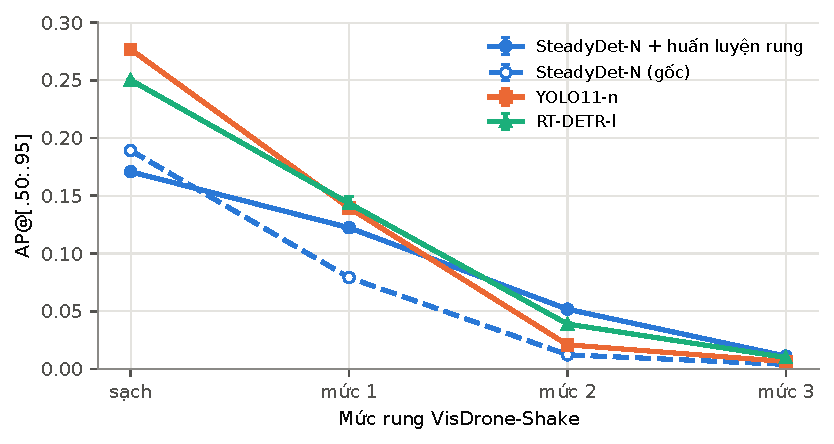
\includegraphics[width=0.94\textwidth]{duong_cong_rung.pdf}
\caption{AP@[.50:.95] theo mức rung. Mô hình gốc (nét đứt) có AP sạch cao hơn nhưng giảm nhanh nhất; sau huấn luyện nhận biết rung (nét liền xanh), SteadyDet-N vượt YOLO11-n và RT-DETR-l từ mức rung 2. Thanh sai số: độ lệch chuẩn qua 3 hạt giống}
\label{fig:duongcong}
\end{figure}

\section{Tính tổng quát và giới hạn của phương pháp}
\label{sec:tongquat}

\subsection{Lặp lại trên một kiến trúc khác}

Một phương pháp chỉ có tác dụng trên đúng một kiến trúc thì khó phân biệt với một sự tương tác may mắn. Khối giữa của Bảng~\ref{tab:ketquachinh} lặp lại thí nghiệm trên SteadyDet-W, mô hình có nhánh $P_2$ đầy đủ, head năm lớp tích chập và chi phí gấp 2,8 lần, mà không chỉnh lại siêu tham số nào. Retain tăng từ $22{,}2 \pm 0{,}9\%$ lên $39{,}4 \pm 0{,}3\%$, tức +17,2 điểm so với +19,3 điểm ở SteadyDet-N; biến thể ràng buộc nhất quán lại một lần nữa kém hơn ($30{,}5 \pm 0{,}6\%$). Chiều hướng, độ lớn và thứ tự giữa hai biến thể đều được tái lập trên một mạng có độ rộng, độ sâu và thiết kế head khác.

\subsection{Không có tác dụng trên YOLO11-n}

Khối dưới cùng áp dụng đúng quy trình cho YOLO11-n và kết quả là không có thay đổi: retain từ $21{,}9 \pm 1{,}1\%$ thành $21{,}5 \pm 0{,}8\%$, đối chứng không rung $21{,}4 \pm 0{,}9\%$. Trên checkpoint YOLO11-n được huấn luyện sẵn trên COCO, phương pháp cho $20{,}1\%$ thành $20{,}1\%$, còn biến thể nhất quán cho $19{,}2\%$. Nhật ký huấn luyện xác nhận toán tử rung đã thực sự được áp dụng. Nhóm đã kiểm tra ba giả thuyết và cả ba đều bị bác bỏ:
\begin{itemize}
\item \textit{Do huấn luyện sẵn trên COCO}: nếu mô hình đã có sẵn đặc trưng chịu được nhoè thì không còn gì để học. Huấn luyện YOLO11-n từ khởi tạo ngẫu nhiên vẫn cho kết quả không đổi, và checkpoint huấn luyện sẵn lại là bản \textit{kém} bền hơn (20,1\% so với 21,9\%).
\item \textit{Do kích thước vật}: có thể chỉ mức bước 4 mới hưởng lợi. Nhưng khi tách riêng vật nhỏ, mức tăng của SteadyDet-N là +18,7 điểm so với +19,3 điểm tổng thể, và gần như mọi người trong tập đều là vật nhỏ với cả hai họ mô hình (AP$_s$ của YOLO11-n là 0,2741 trên AP 0,2768).
\item \textit{Do khoảng trống còn lại}: SteadyDet-W bắt đầu từ $22{,}2 \pm 0{,}9\%$ và YOLO11-n từ đầu bắt đầu từ $21{,}9 \pm 1{,}1\%$, gần như cùng điểm xuất phát, nhưng một mô hình tăng 17,2 điểm, mô hình kia không tăng.
\end{itemize}
Nguyên nhân còn lại nằm ở kiến trúc hoặc hàm mất mát mà hai mô hình của đề tài có chung còn YOLO11-n thì không: mức bước 4, hàm mất mát NWD kết hợp CIoU, QFL, và hồi quy hộp trực tiếp thay vì theo phân phối. Một mô hình không phản hồi không đủ để tách các yếu tố này, nên đề tài phát biểu kết luận đúng phạm vi bằng chứng: phương pháp cho mức tăng lớn và tái lập được trên họ kiến trúc của đề tài, và không có tác dụng trên mô hình ngoài họ đã thử.

Kết quả âm này cũng có một vai trò quan trọng: nó làm cho phép so sánh ở mục sau trở nên công bằng. Vì phương pháp không nâng được YOLO11-n, việc so sánh ``SteadyDet-N có xử lý'' với ``YOLO11-n không xử lý'' không phải là so với một đối thủ bị làm yếu đi.

\section{So sánh với các mô hình phát hiện nhẹ}
\label{sec:sosanh}

\begin{table}[H]
\centering
\caption{So sánh với năm mô hình công khai trên VisDrone-person, mọi dòng đo bằng cùng một chương trình. mCP: AP@[.50:.95] trung bình ba mức rung, tức độ chính xác \textit{khi bay}. Các mô hình YOLO và RT-DETR khởi tạo từ trọng số huấn luyện sẵn trên COCO, còn SteadyDet huấn luyện từ đầu, điều này có lợi cho mô hình đối chứng}
\label{tab:sosanh}
\small
\setlength{\tabcolsep}{4pt}
\renewcommand{\arraystretch}{1.15}
\begin{tabular}{@{}lcccccc@{}}
\toprule
\textbf{Mô hình} & \textbf{Tham số (M)} & \textbf{GFLOPs} & \textbf{AP$_{50}$} & \textbf{AP} & \textbf{mCP} & \textbf{retain (\%)}\\
\midrule
RT-DETR-l~\cite{zhao2024rtdetr} & 32,81 & 108,0 & 0,5909 & 0,2502$^{\dagger}$ & 0,0641 & \ms{25,6}{1,1}\\
YOLOv10-n~\cite{wang2024yolov10} & 2,71 & 8,4 & 0,6043 & 0,2730 & 0,0538 & \ms{19,7}{1,4}\\
YOLOv8-n~\cite{ultralytics} & 3,01 & 8,2 & 0,6033 & 0,2684 & 0,0522 & \ms{19,5}{0,8}\\
YOLO26-n~\cite{ultralytics} & 2,50 & 5,8 & 0,5898 & 0,2675 & 0,0507 & \ms{19,0}{1,0}\\
YOLO11-n~\cite{ultralytics} & 2,59 & 6,4 & \textbf{0,6119} & \textbf{0,2768} & 0,0557 & \ms{20,1}{1,2}\\
\quad + huấn luyện nhận biết rung & 2,59 & 6,4 & 0,6057 & 0,2700 & 0,0542 & \ms{20,1}{1,3}\\
\midrule
SteadyDet-W (gốc) & 1,00 & 12,9 & 0,5800 & 0,2349 & 0,0521 & \ms{22,2}{0,9}\\
\quad \textbf{+ huấn luyện nhận biết rung} & 1,00 & 12,9 & 0,5511 & 0,2219 & \textbf{0,0874} & \textbf{\ms{39,4}{0,3}}\\
SteadyDet-N (gốc) & \textbf{1,17} & \textbf{4,6} & 0,5127 & 0,1892 & 0,0318 & \ms{16,8}{0,7}\\
\quad + ràng buộc nhất quán & 1,17 & 4,6 & 0,4837 & 0,1746 & 0,0524 & \ms{30,0}{0,6}\\
\quad \textbf{+ huấn luyện nhận biết rung} & \textbf{1,17} & \textbf{4,6} & 0,4731 & 0,1708 & \textbf{0,0617} & \textbf{\ms{36,2}{0,7}}\\
\bottomrule
\multicolumn{7}{@{}p{0.98\textwidth}@{}}{\footnotesize $^{\dagger}$ Bộ tiền xử lý gốc của RT-DETR kéo giãn ảnh thay vì đệm xám; trong đường xử lý chung, AP sạch của nó bị kéo xuống (chương trình gốc cho 0,3340). mCP và retain là tỷ số trong cùng một đường xử lý nên không bị ảnh hưởng.}\\
\end{tabular}
\end{table}

\subsection{Trên ảnh sạch, SteadyDet-N không dẫn đầu}

Cả bốn mô hình YOLO bản nano đều có AP sạch cao hơn SteadyDet-N, và đề tài không né tránh điều đó. Việc các mô hình đối chứng được khởi tạo từ trọng số huấn luyện sẵn trên COCO là một yếu tố, nhưng khoảng cách lớn hơn mức mà yếu tố này có thể giải thích. Hiệu quả tính toán cũng không bù được: 4,6 GFLOPs so với 5,8 GFLOPs của mô hình đối chứng rẻ nhất (YOLO26-n) chỉ tiết kiệm 21\%. Nếu chỉ xét benchmark trên ảnh sạch, SteadyDet-N thua.

\subsection{Khi rung, thứ hạng đảo ngược}

Cột mCP xếp hạng bảng gần như ngược với cột AP sạch. SteadyDet-N có huấn luyện nhận biết rung đạt mCP 0,0617, cao hơn mô hình đối chứng nhỏ tốt nhất là YOLO11-n (0,0557), trong khi chỉ dùng 45\% số tham số và 72\% chi phí tính toán của nó. \textbf{SteadyDet-N vượt cả bốn mô hình YOLO bản nano về độ chính xác khi bay.}

RT-DETR-l có mCP trung bình cao hơn SteadyDet-N (0,0641 so với 0,0617), nhưng không phải ở điều kiện quan trọng nhất. Ở mức rung 2, tương ứng bay tiến thông thường, RT-DETR-l đạt $0{,}0389 \pm 0{,}0014$ còn SteadyDet-N đạt $0{,}0518 \pm 0{,}0019$, chênh lệch khoảng 5,5 lần độ lệch chuẩn gộp, trong khi RT-DETR-l có số tham số gấp 28 lần và chi phí gấp 23 lần. Ở mức 3, hai mô hình nằm trong phạm vi nhiễu ($0{,}0100 \pm 0{,}0017$ so với $0{,}0111 \pm 0{,}0002$), nên đề tài không kết luận thứ tự ở mức này. So với YOLO11-n ở mức 2, SteadyDet-N hơn 2,5 lần (0,0518 so với 0,0210).

SteadyDet-W có huấn luyện nhận biết rung dẫn đầu toàn bảng với mCP 0,0874. Tuy vậy, đề tài chọn SteadyDet-N làm mô hình chính vì trên nền tảng đích, ràng buộc chặt nhất là chi phí tính toán chứ không phải số tham số: mô hình, bộ theo vết và bộ điều khiển phải cùng vừa một khung thời gian. Tính trên mỗi GFLOP, thứ tự rất rõ ràng: SteadyDet-N đạt 0,0134 mCP/GFLOP, so với 0,0087 của YOLO11-n và 0,0068 của SteadyDet-W.

\begin{figure}[H]
\centering
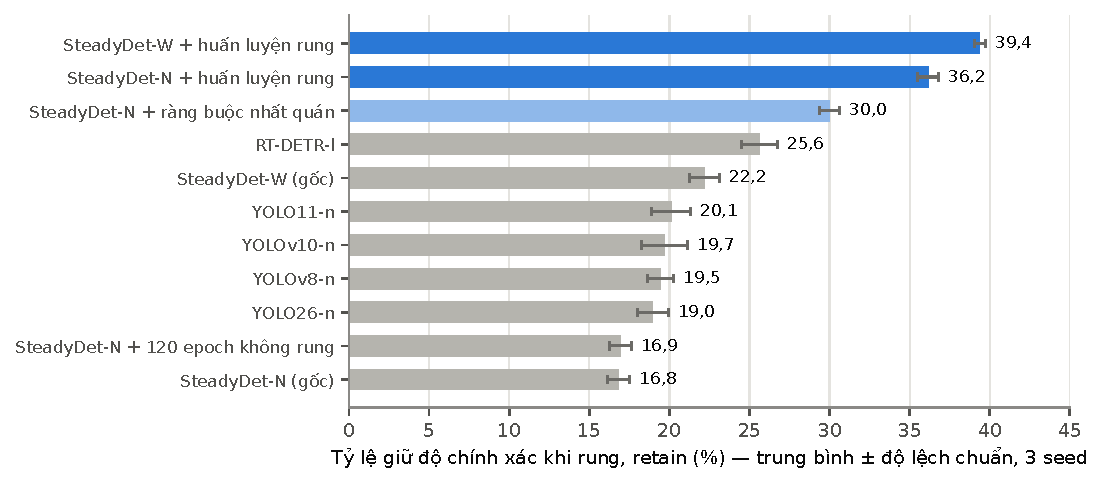
\includegraphics[width=0.94\textwidth]{retain.pdf}
\caption{Tỷ lệ giữ độ chính xác khi rung của mọi mô hình. Bốn thế hệ YOLO bản nano nằm sát nhau ở 19--20\% dù khác nhau về kiến trúc; hai mô hình của đề tài sau huấn luyện nhận biết rung đứng đầu}
\label{fig:retain}
\end{figure}

\subsection{Độ bền không phải là sản phẩm phụ của độ chính xác}

Hình~\ref{fig:danhdoi} biểu diễn AP sạch theo mCP. Các mô hình công khai tập trung ở góc phải dưới: độ chính xác sạch cao hơn nhưng không bền hơn; bốn thế hệ YOLO trải dài bốn năm và ba trường phái thiết kế nhưng retain chỉ cách nhau khoảng một điểm phần trăm. RT-DETR-l đạt 25,6\% nhờ số tham số gấp 28 lần. Hendrycks và Dietterich đã ghi nhận hiện tượng tương tự với mô hình phân loại ImageNet~\cite{hendrycks2019imagenetc}: độ bền tương đối gần như không cải thiện qua nhiều năm tiến bộ kiến trúc. Kết quả của đề tài cho thấy điều này cũng đúng với bộ phát hiện nhẹ trên ảnh UAV. Hệ quả thực tiễn là \textbf{độ bền phải được đo và tối ưu riêng}; các mũi tên trong hình cho thấy thay đổi phân phối huấn luyện mang lại mức tăng độ bền lớn với mức giảm độ chính xác sạch nhỏ.

\begin{figure}[H]
\centering
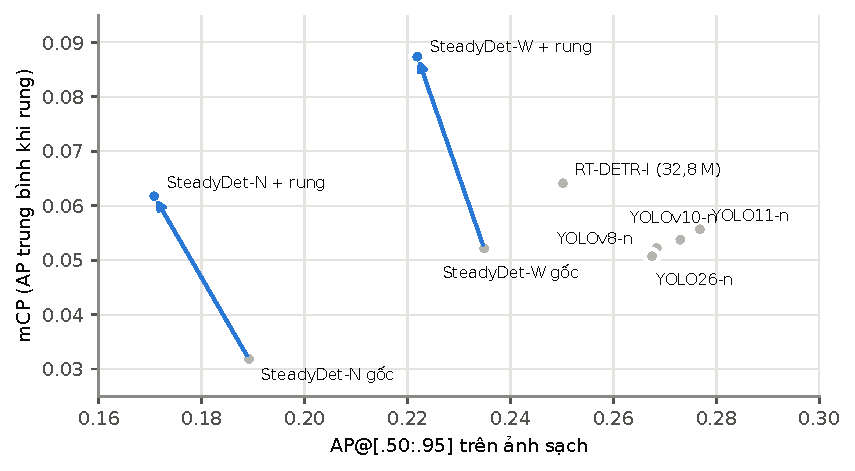
\includegraphics[width=0.94\textwidth]{danh_doi.pdf}
\caption{AP trên ảnh sạch và mCP khi rung, mỗi điểm là một mô hình. Mũi tên xanh: tác dụng của huấn luyện nhận biết rung trên hai mô hình của đề tài}
\label{fig:danhdoi}
\end{figure}

\section{Kiểm chứng trên dữ liệu bay thật}
\label{sec:baythat}

Mọi kết quả ở trên dựa trên suy giảm mô phỏng. Mục này dùng 92 khung hình bay thật ở độ cao khoảng 6\,m, nơi nhoè do chính máy bay tạo ra. Sáu mô hình SteadyDet-N có cùng kiến trúc được so sánh theo hai trục độc lập: dữ liệu huấn luyện (có hay không có COCO-person) và cách xử lý rung.

\begin{table}[H]
\centering
\caption{Kết quả trên 92 khung hình bay thật ($\approx$6\,m), cùng chương trình đo. Trong mỗi nhóm, ba mô hình giống hệt kiến trúc và chỉ khác cách xử lý rung}
\label{tab:baythat}
\small
\renewcommand{\arraystretch}{1.15}
\begin{tabular}{@{}llcccc@{}}
\toprule
\textbf{Dữ liệu huấn luyện} & \textbf{Xử lý rung} & \textbf{AP$_{50}$} & \textbf{AP} & \textbf{AP$_{75}$} & \textbf{AR$_{100}$}\\
\midrule
VisDrone + COCO-person & không & 0,7613 & 0,3369 & 0,1448 & 0,5076\\
VisDrone + COCO-person & huấn luyện nhận biết rung & 0,7747 & 0,3792 & 0,2583 & \textbf{0,5315}\\
VisDrone + COCO-person & ràng buộc nhất quán & \textbf{0,8798} & \textbf{0,3885} & \textbf{0,2620} & 0,5087\\
\midrule
Chỉ VisDrone & không & 0,1435 & 0,0547 & 0,0166 & 0,4315\\
Chỉ VisDrone & huấn luyện nhận biết rung & 0,0579 & 0,0207 & 0,0076 & 0,4076\\
Chỉ VisDrone & ràng buộc nhất quán & 0,0909 & 0,0283 & 0,0093 & 0,3772\\
\bottomrule
\end{tabular}
\end{table}

\begin{figure}[H]
\centering
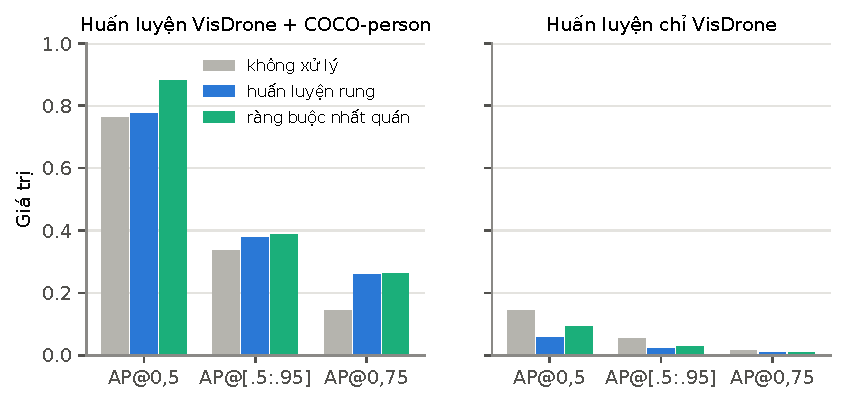
\includegraphics[width=0.94\textwidth]{bay_that.pdf}
\caption{Kết quả trên dữ liệu bay thật theo nhóm dữ liệu huấn luyện. Nhóm có COCO-person (trái) chính xác gấp nhiều lần nhóm chỉ VisDrone (phải); trong nhóm có COCO, cả hai cách xử lý rung làm AP@0,75 tăng gần gấp đôi}
\label{fig:baythat}
\end{figure}

\subsection{Cả hai cách xử lý rung đều có tác dụng trên rung thật}

Trong nhóm mô hình phù hợp với miền này (có COCO-person), cả hai cách xử lý đều cải thiện theo cùng một kiểu. AP@0,75 tăng từ 0,1448 lên 0,2583 với huấn luyện nhận biết rung và 0,2620 với ràng buộc nhất quán, tức tăng tương đối 78\% và 81\% ở độ khít hộp, trong khi recall gần như không đổi (0,5076 thành 0,5315 và 0,5087). Mô hình không tìm thấy thêm người; nó đặt hộp khít hơn quanh những người đã tìm thấy, đúng dấu hiệu mong đợi nếu mô hình học được cách nhìn xuyên qua nhoè.

Để kiểm tra ý nghĩa thống kê trên 92 khung, đề tài lấy mẫu lại khung hình 1.000 lần theo cặp. Khoảng tin cậy 95\% của hiệu so với mô hình không xử lý:
\begin{itemize}
\item huấn luyện nhận biết rung: AP +0,042 [+0,011; +0,074], AP@0,75 +0,108 [+0,010; +0,211];
\item ràng buộc nhất quán: AP +0,051 [+0,012; +0,087], AP@0,75 +0,110 [+0,012; +0,214], AP@0,5 +0,119 [+0,071; +0,173].
\end{itemize}
Mọi khoảng tin cậy trên đều không chứa 0, nên cả hai cách xử lý thực sự tốt hơn mô hình không xử lý trên dữ liệu này. Hai cách xử lý chỉ tách nhau ở AP@0,5 (+0,106 [+0,058; +0,161] nghiêng về ràng buộc nhất quán), còn hiệu AP và AP@0,75 giữa chúng đều chứa 0. Thứ tự ở AP@0,5 ngược với thứ tự trên VisDrone-Shake. Với một người, một cảnh và một độ cao, dữ liệu này không đủ để quyết định thứ tự nào tổng quát hơn; câu trả lời cần một tập bay lớn hơn.

\subsection{Chọn dữ liệu theo miền triển khai, không theo benchmark}

Thêm COCO-person làm AP@0,5 trên dữ liệu bay thật tăng 5,3 lần (0,1435 lên 0,7613), trong khi trên VisDrone-val cùng thay đổi này lại \textit{làm giảm} AP@0,5 (0,5127 xuống 0,5016). Phân tích chi tiết giải thích cơ chế: mô hình chỉ học VisDrone vẫn có recall khá (0,4315), tức vẫn thấy người, nhưng định vị sụp đổ (AP@0,75 chỉ 0,0166) vì chưa từng được học trên người chiếm phần lớn khung hình. Nếu chọn dữ liệu huấn luyện dựa trên benchmark, nhóm sẽ chọn đúng mô hình sai. Với bài toán bám theo người ở cự ly gần, dữ liệu huấn luyện phải khớp với dải độ cao triển khai.

Trong nhóm chỉ VisDrone, thứ tự đảo ngược (AP@0,5 giảm từ 0,1435 xuống 0,0909 và 0,0579). Cả ba mô hình này đều thất bại ở miền bay thấp, nên so sánh giữa chúng là so sánh giữa các cách thất bại: làm cho biểu diễn bền trước nhoè chỉ có ích khi biểu diễn đó vốn đã phù hợp. Huấn luyện nhận biết rung là phương pháp tăng độ bền, không phải phương pháp thích nghi miền.

\section{Thảo luận}

Bốn kết luận chính rút ra từ chương này:
\begin{enumerate}
\item Rung là điều kiện luôn có khi bay, và dưới một giao thức đo thống nhất, mọi bộ phát hiện nhỏ gọn đều mất phần lớn độ chính xác. Vấn đề thuộc về điều kiện vận hành chứ không thuộc về một kiến trúc cụ thể.
\item Huấn luyện nhận biết rung tăng retain của SteadyDet-N từ 16,8\% lên 36,2\% và AP ở mức rung 2 lên 4,2 lần, không tốn chi phí suy luận; đối chứng xác nhận tác dụng không đến từ việc huấn luyện thêm.
\item Kiến trúc và phương pháp huấn luyện đều cần thiết: SteadyDet-N không xử lý đứng cuối bảng về mCP, còn phương pháp áp dụng lên YOLO11-n không có tác dụng. Chỉ khi kết hợp cả hai, mô hình nhỏ nhất và rẻ nhất mới vượt cả bốn mô hình YOLO bản nano khi rung.
\item Trên dữ liệu bay thật, xử lý rung làm hộp khít hơn rõ rệt, và dữ liệu huấn luyện phù hợp miền triển khai quan trọng hơn thứ hạng trên benchmark.
\end{enumerate}

Các giới hạn cần nêu rõ: toán tử rung là mô hình mô phỏng, tham số được chọn để bao quát điều kiện bay chứ chưa hiệu chuẩn theo phổ gia tốc đo trên chính khung máy bay; mỗi cấu hình chỉ được huấn luyện một lần nên thanh sai số phản ánh biến động của phép đo chứ chưa phản ánh biến động của huấn luyện; tập bay thật mới có một người, một cảnh, một độ cao. Các giới hạn này được đưa vào phần kiến nghị.

% =====================================================================
%  CHƯƠNG 5. TRIỂN KHAI MÔ HÌNH TRÊN THIẾT BỊ BIÊN
%  Nguồn số: runs/pi_hailo_measured_2026-08-24.md, runs/pi_camera_measured_2026-08-27.md,
%            runs/flight_val_hef_2026-08-27.md, runs/retrain_coco_2026-08-27.md
% =====================================================================
\chapter{Triển khai mô hình trên thiết bị biên}
\label{chap:trienkhai}

Một mô hình chính xác trên máy tính huấn luyện chưa chắc dùng được trên máy bay. Chương này trình bày quá trình đưa SteadyDet-N lên Raspberry Pi~5 gắn NPU Hailo-8L: chuẩn bị mô hình cho trình biên dịch, lượng tử hoá INT8, đo độ chính xác sau lượng tử hoá trên hai miền dữ liệu, đo tốc độ và độ trễ đầu-cuối với camera thật. Mọi con số trong chương đều được đo trực tiếp trên phần cứng đích.

\section{Nền tảng phần cứng}

Máy tính đồng hành là Raspberry Pi~5 chạy Debian~12. NPU Hailo-8L gắn qua khe M.2 và đường PCIe; trong cấu hình đo, liên kết hoạt động ở tốc độ Gen2 x1 (5\,GT/s). Camera là Logitech C270 HD cắm cổng USB, dùng định dạng nén MJPG. Bộ điều khiển bay Pixhawk~6C nối với Pi qua USB. Phần suy luận chạy trên NPU; các phần còn lại (đọc camera, tiền xử lý, giải mã, NMS, theo vết, điều khiển, bảng giám sát web) chạy trên CPU của Pi.

\begin{figure}[H]
\centering
\resizebox{\textwidth}{!}{% Quy trình đưa mô hình từ PyTorch lên NPU Hailo-8L
\begin{tikzpicture}[
  font=\footnotesize, >={Stealth[length=2mm]},
  st/.style={draw=black!60, rounded corners=2pt, align=center, minimum height=11mm, text width=2.45cm, inner sep=2pt, fill=white},
  pc/.style={st, fill=black!5},
  hw/.style={st, fill=xanh!14},
  note/.style={font=\scriptsize, text=black!70, align=center, text width=2.5cm}
]
\node[pc] (a) {Checkpoint PyTorch\\(FP32, bỏ self-attention)};
\node[pc, right=6mm of a] (b) {Xuất ONNX\\opset 11, kích thước tĩnh};
\node[pc, right=6mm of b] (c) {DFC: phân tích đồ thị\\4 bản đồ đầu ra};
\node[pc, right=6mm of c] (d) {DFC: lượng tử hoá INT8\\64 ảnh hiệu chuẩn (tập huấn luyện)};
\node[pc, right=6mm of d] (e) {DFC: biên dịch\\$\rightarrow$ tệp HEF (4 context)};
\foreach \x/\y in {a/b,b/c,c/d,d/e} \draw[->] (\x) -- (\y);
\node[note, below=1mm of a] {tinh chỉnh 20 epoch\\có COCO-person};
\node[note, below=1mm of b] {gộp BN vào Conv,\\\texttt{dynamo=False}};

\node[font=\footnotesize\bfseries, anchor=west] at ($(a.north west)+(0,0.35)$) {Máy tính x86 (biên dịch một lần)};

\node[hw, below=3.0cm of b] (f) {Camera C270\\khung $640\times480$};
\node[hw, right=6mm of f] (g) {Tiền xử lý CPU\\letterbox 640};
\node[hw, right=6mm of g] (h) {Suy luận INT8\\NPU Hailo-8L};
\node[hw, right=6mm of h] (i) {Giải mã + NMS\\CPU (NumPy)};
\foreach \x/\y in {f/g,g/h,h/i} \draw[->] (\x) -- (\y);
\draw[->, dashed] (e.south) -- ++(0,-0.75) -| (h.north);
\node[font=\footnotesize\bfseries, anchor=west] at ($(f.north west)+(0,0.35)$) {Raspberry Pi~5 trên máy bay (mỗi khung hình)};
\end{tikzpicture}
}
\caption{Quy trình đưa mô hình lên NPU: biên dịch một lần trên máy tính x86 (trên) và chuỗi xử lý mỗi khung hình trên Raspberry Pi~5 (dưới)}
\label{fig:quytrinhtrienkhai}
\end{figure}

\section{Chuẩn bị mô hình cho trình biên dịch}

\subsection{Loại bỏ khối self-attention}

Trình biên dịch Hailo DFC không hỗ trợ các phép biến đổi hình dạng tensor mà khối self-attention theo cửa sổ sử dụng. Đề tài xử lý bằng cách tạo một cấu hình SteadyDet-N không có khối này (thuần tích chập, 0,875 triệu tham số) và tinh chỉnh 20 epoch từ checkpoint của nhánh triển khai với learning rate $10^{-3}$. Việc kiểm tra tệp ONNX sau khi xuất xác nhận đồ thị không còn các phép toán MatMul, Softmax hay ReduceMean. Việc chuyển đổi này có ảnh hưởng tới độ chính xác, được định lượng ở mục~\ref{sec:chonhef}.

\subsection{Một lỗi cấu hình và cách phát hiện}

Lần tinh chỉnh đầu tiên cho kết quả kém bất thường trên dữ liệu bay thật: F1 của bản FP32 chỉ đạt 0,768 so với 0,882 của checkpoint trước khi tinh chỉnh. Khi phân tích nhật ký huấn luyện, nhóm nhận thấy toàn bộ mẫu dương đều rơi vào hai mức $P_2$ và $P_3$ (số mẫu dương ở $P_4$ và $P_5$ bằng 0), tức mô hình không hề thấy người kích thước lớn trong suốt quá trình tinh chỉnh. Nguyên nhân là tệp cấu hình đặt epoch bắt đầu trộn COCO-person bằng 100 trong khi toàn bộ quá trình chỉ có 20 epoch, nên dữ liệu người cự ly gần chưa bao giờ được bật. Sau khi sửa để trộn COCO ngay từ epoch đầu, nhật ký xác nhận có mẫu dương ở cả $P_4$ và $P_5$, và F1 trên dữ liệu bay thật tăng từ 0,768 lên 0,836, lấy lại 60\% khoảng cách. Phần chênh lệch còn lại (0,046) là cái giá của việc bỏ khối self-attention trên miền bay thấp. Bài học rút ra là: kiểm tra phân bố mẫu dương theo mức là một cách rẻ để phát hiện dữ liệu huấn luyện không đúng như ý định.

\subsection{Xuất ONNX}

Mô hình được gộp các lớp batch norm vào tích chập, xuất ONNX với kích thước đầu vào tĩnh $640\times640$ và opset 11. Đầu ra là bốn bản đồ dự đoán thô; phần giải mã theo phương trình~(\ref{eq:decode}) và NMS chạy trên CPU. Nhóm gặp một lỗi khi xuất: từ PyTorch 2.6, hàm xuất ONNX mặc định dùng bộ xuất mới, bộ này bỏ thuộc tính \texttt{kernel\_shape} của nút tích chập (vẫn hợp lệ theo chuẩn ONNX) nhưng trình phân tích của Hailo lại đọc trực tiếp thuộc tính này và dừng với lỗi chỉ số. Buộc dùng bộ xuất cũ (\texttt{dynamo=False}) cho tệp opset 11 với đủ 82/82 nút tích chập có thuộc tính này. Để chắc chắn tệp ONNX tương đương PyTorch, nhóm chạy toàn bộ phép quét ngưỡng trên dữ liệu bay thật bằng cả hai: F1 đạt 0,831 (ONNX) so với 0,836 (PyTorch), số dự đoán đúng giống hệt ở mọi ngưỡng.

\section{Lượng tử hoá và biên dịch}

Tệp ONNX được DFC lượng tử hoá INT8 với mức tối ưu 2 và biên dịch thành tệp HEF gồm 4 context. Tập ảnh hiệu chuẩn được lấy từ \textit{tập huấn luyện}, trộn đúng tỷ lệ dùng khi huấn luyện (75\% VisDrone, 25\% COCO-person). Tập flight\_val không được dùng để hiệu chuẩn vì đó là tập đánh giá. Nhóm biên dịch hai phiên bản: một với 64 ảnh hiệu chuẩn và một với 512 ảnh.

\section{Độ chính xác sau lượng tử hoá}
\label{sec:int8}

\subsection{Chọn tệp HEF triển khai}
\label{sec:chonhef}

Ba tệp HEF được đo trên Pi, cùng 92 khung bay thật và cùng một đường giải mã (Bảng~\ref{tab:hef}).

\begin{table}[H]
\centering
\caption{So sánh các tệp HEF trên 92 khung bay thật; mỗi tệp dùng ngưỡng tin cậy cho F1 cao nhất của chính nó}
\label{tab:hef}
\small
\renewcommand{\arraystretch}{1.15}
\begin{tabularx}{\textwidth}{@{}>{\raggedright\arraybackslash}Xcccccc@{}}
\toprule
\textbf{Tệp HEF} & \textbf{Ảnh hiệu chuẩn} & \textbf{Ngưỡng} & \textbf{F1} & \textbf{Độ phủ} & \textbf{Độ chuẩn xác} & \textbf{FPS}\\
\midrule
\textbf{Có COCO, 64 ảnh (triển khai)} & 64 & 0,25 & \textbf{0,880} & \textbf{0,837} & 0,928 & 56,9\\
Có COCO, 512 ảnh & 512 & 0,25 & 0,812 & 0,750 & 0,885 & 62,9\\
Bản trước (chưa trộn COCO) & -- & 0,30 & 0,745 & 0,620 & 0,934 & 63,7\\
\bottomrule
\end{tabularx}
\end{table}

Tệp dùng 64 ảnh hiệu chuẩn cho F1 cao nhất và recall 0,837, tức bắt được người ở 84\% số khung thay vì 62\% như bản trước. Nó chậm hơn khoảng 2\,ms mỗi khung (17,6\,ms so với 15,7\,ms) nhưng vẫn dư xa ngân sách 33,3\,ms, nên được chọn để triển khai. Một kết quả trái trực giác: 512 ảnh hiệu chuẩn cho kết quả kém hơn 64 ảnh, dù trình biên dịch khuyến nghị nhiều ảnh hơn. Nhóm chưa xác định được cơ chế; bài học vận hành là phải đo trên dữ liệu miền triển khai thay vì dựa vào khuyến nghị chung.

\subsection{Tổn thất INT8 phụ thuộc kích thước đối tượng}

Để đo đúng tổn thất do lượng tử hoá, dự đoán FP32 (trên GPU) và INT8 (trên NPU) của cùng một mô hình được xuất ra cùng một định dạng và chấm bằng cùng một hàm, trên cả hai miền dữ liệu (Bảng~\ref{tab:int8}, Hình~\ref{fig:int8}).

\begin{table}[H]
\centering
\caption{Độ chính xác FP32 và INT8 của mô hình triển khai, cùng một chương trình chấm điểm}
\label{tab:int8}
\small
\renewcommand{\arraystretch}{1.15}
\begin{tabular}{@{}lccc|ccc@{}}
\toprule
 & \multicolumn{3}{c|}{\textbf{VisDrone-val (548 ảnh, người rất nhỏ)}} & \multicolumn{3}{c}{\textbf{Bay thật $\approx$6\,m (92 khung)}}\\
\textbf{Chỉ số} & \textbf{FP32} & \textbf{INT8} & \textbf{Thay đổi} & \textbf{FP32} & \textbf{INT8} & \textbf{Thay đổi}\\
\midrule
AP@[.50:.95] & 0,1775 & 0,1584 & $-$10,8\% & 0,4356 & 0,4349 & $-$0,2\%\\
AP@0,50 & 0,4946 & 0,4625 & $-$6,5\% & 0,8822 & \textbf{0,9171} & +4,0\%\\
AP@0,75 & 0,0742 & 0,0555 & $-$25,2\% & 0,2561 & 0,2552 & $-$0,4\%\\
AR@100 & 0,3041 & 0,2869 & $-$5,7\% & 0,5489 & 0,5337 & $-$2,8\%\\
\bottomrule
\end{tabular}
\end{table}

\begin{figure}[H]
\centering
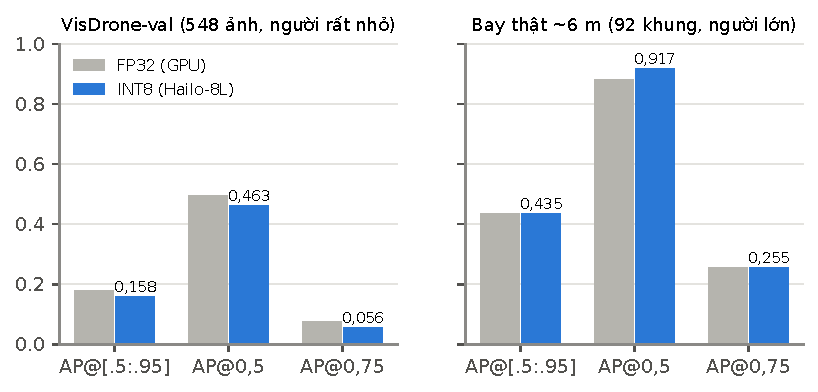
\includegraphics[width=\textwidth]{int8.pdf}
\caption{Độ chính xác FP32 và INT8 trên hai miền dữ liệu. Trên người rất nhỏ, INT8 làm hộp kém khít (AP@0,75 giảm 25\%); trên người ở độ cao bay thực tế, hai bản gần như trùng nhau}
\label{fig:int8}
\end{figure}

Trên VisDrone-val, AP@0,5 chỉ giảm 6,5\% còn AP@0,75 giảm 25,2\%: lượng tử hoá không làm mất đối tượng mà làm hộp kém khít. Điều này phù hợp với phân tích ở Chương~\ref{chap:lythuyet}: điểm tin cậy chịu được lượng tử hoá, còn toạ độ hộp mất độ phân giải, và với người chỉ vài điểm ảnh, sai lệch nhỏ đó đủ làm IoU tụt dưới 0,75. Trên dữ liệu bay thật, người chiếm hàng nghìn điểm ảnh nên cùng sai lệch gần như không đáng kể: hai bản khác nhau không quá 0,035 ở mọi chỉ số, nằm trong sai số lấy mẫu của 92 khung. Phát biểu chính xác là: \textbf{INT8 tốn khoảng 6,5\% AP@0,5 với người rất nhỏ và gần như không tốn gì với người ở độ cao bay 3--6\,m}. Kết quả này cũng điều chỉnh một kết luận bi quan trước đó của nhóm, khi lượng tử hoá sau huấn luyện đơn giản trên ONNX từng làm AP sụp từ 0,18 xuống 0,009; hiệu chuẩn theo từng lớp của DFC tốt hơn nhiều.

\textbf{Chỉ tiêu độ chính xác của đề tài.} Mô hình đang chạy trên máy bay đạt AP@0,5 = 0,917 trên dữ liệu bay thật, vượt chỉ tiêu 70\% trong thuyết minh. Con số này là của đúng mô hình INT8 trên NPU chứ không phải của một checkpoint trên máy tính huấn luyện. Lưu ý không so sánh trực tiếp con số 0,917 với 0,7613 ở Bảng~\ref{tab:baythat}: hai con số thuộc hai checkpoint khác nhau và được tính bằng hai đường giải mã khác nhau; Bảng~\ref{tab:baythat} dùng để so sánh \textit{dữ liệu và cách xử lý rung}, còn Bảng~\ref{tab:int8} dùng để đánh giá \textit{hệ thống triển khai}.

\subsection{Chọn ngưỡng tin cậy vận hành}

Ngưỡng tin cậy quyết định trực tiếp hành vi trên máy bay: quá cao thì bỏ sót người, quá thấp thì bám nhầm vào hộp sai. Với bản HEF trước, ngưỡng 0,40 chỉ bắt được người ở 19,6\% số khung, còn ngưỡng 0,20 sinh trung bình 1,30 hộp sai mỗi khung, khớp đúng hiện tượng người dùng quan sát được khi thử (``chĩa vào người không thấy gì'' và ``hạ ngưỡng thì nhiễu''). Hình~\ref{fig:nguong} là kết quả quét ngưỡng cho bản HEF triển khai: F1 đạt cực đại 0,880 tại ngưỡng 0,25 và giảm còn 0,551 ở ngưỡng 0,40. Ngưỡng tối ưu thay đổi theo từng tệp HEF (bản trước là 0,30), nên mỗi lần đổi mô hình phải quét lại.

\begin{figure}[H]
\centering
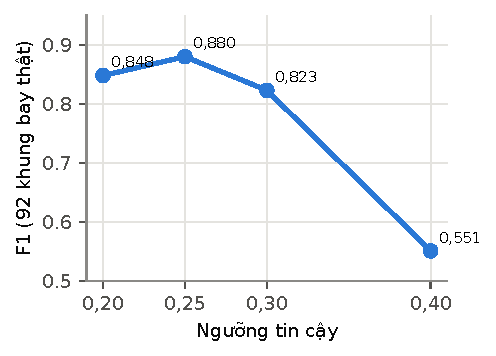
\includegraphics[width=0.5\textwidth]{nguong_conf.pdf}
\caption{F1 của mô hình triển khai theo ngưỡng tin cậy trên 92 khung bay thật}
\label{fig:nguong}
\end{figure}

\section{Tốc độ suy luận trên NPU}

\subsection{Tốc độ theo từng khung và theo lô}

Tốc độ được đo bằng công cụ chuẩn \texttt{hailortcli benchmark} của Hailo và kiểm tra chéo bằng lời gọi đồng bộ từ Python; hai cách cho kết quả khớp nhau. Với batch size 1, SteadyDet-N đạt \textbf{112,55 FPS (8,40\,ms)} ở $320\times320$ và \textbf{63,66 FPS (15,26\,ms)} ở $640\times640$. Bản HEF triển khai đạt 56,9 FPS, độ trễ suy luận trung vị 17,32\,ms và p99 17,52\,ms đo trong lượt đánh giá 548 ảnh.

\begin{table}[H]
\centering
\caption{Thông lượng và độ trễ theo batch size trên Hailo-8L (mô hình $320\times320$)}
\label{tab:batch}
\small
\renewcommand{\arraystretch}{1.15}
\begin{tabular}{@{}ccc@{}}
\toprule
\textbf{Kích thước lô} & \textbf{Thông lượng (FPS)} & \textbf{Độ trễ phần cứng (ms)}\\
\midrule
1 & 112,55 & 8,40\\
4 & 188,78 & 17,05\\
8 & 214,63 & 28,35\\
16 & 231,82 & 50,48\\
\bottomrule
\end{tabular}
\end{table}

Bảng~\ref{tab:batch} cho thấy tăng batch size làm tăng thông lượng nhưng cũng làm tăng độ trễ mỗi khung. Hệ thống bám người dùng lô 1 vì hai lý do: độ trễ phần cứng tăng từ 8,40 lên 17,05\,ms ở lô 4, và với camera 30 khung/giây, riêng việc chờ gom đủ 4 khung đã mất thêm 133\,ms, một độ trễ mà vòng điều khiển bám người không chấp nhận được. Thông lượng và độ trễ là hai đại lượng khác nhau và không được nhầm lẫn khi báo cáo.

\subsection{So sánh với YOLO26-n trên cùng một chip}

Để kiểm tra luận điểm hiệu quả tính toán trên phần cứng thật, đề tài biên dịch YOLO26-n (chính checkpoint dùng trong Bảng~\ref{tab:sosanh}) bằng đúng cùng lệnh và tham số, cắt đồ thị tại các tích chập đầu ra để phần giải mã và NMS của cả hai mô hình đều chạy trên CPU, rồi đo trên cùng Pi.

\begin{table}[H]
\centering
\caption{SteadyDet-N và YOLO26-n trên cùng Hailo-8L, ảnh $640\times640$, lô 1}
\label{tab:yolo26hailo}
\small
\renewcommand{\arraystretch}{1.15}
\begin{tabular}{@{}lccccc@{}}
\toprule
\textbf{Mô hình} & \textbf{Tham số (M)} & \textbf{GFLOPs} & \textbf{Số context} & \textbf{FPS} & \textbf{Độ trễ (ms)}\\
\midrule
\textbf{SteadyDet-N} & \textbf{1,17} & \textbf{4,6} & \textbf{4} & \textbf{63,66} & \textbf{15,26}\\
YOLO26-n & 2,38 & 5,2 & 6 & 37,46 & 24,79\\
\bottomrule
\end{tabular}
\end{table}

SteadyDet-N \textbf{nhanh hơn 1,70 lần} với 49\% số tham số và 88\% chi phí tính toán (Bảng~\ref{tab:yolo26hailo}, Hình~\ref{fig:hailo}). Mức chênh lệch tốc độ lớn hơn nhiều so với mức chênh lệch GFLOPs; cơ chế nằm ở số context: SteadyDet-N vừa 4 context còn YOLO26-n cần 6, và mỗi lần chuyển context NPU phải nạp lại trọng số qua PCIe. Trên loại chip này, giảm kích thước mô hình để giảm số context quan trọng không kém giảm số phép tính. Hai tệp HEF trong phép so sánh này được hiệu chuẩn bằng ảnh kiểm định, nên chỉ dùng để so tốc độ, không dùng để lấy độ chính xác. Số tham số và GFLOPs của YOLO26-n ở đây được tính trên đồ thị đã xuất để biên dịch, nên khác một chút so với Bảng~\ref{tab:sosanh}.

\begin{figure}[H]
\centering
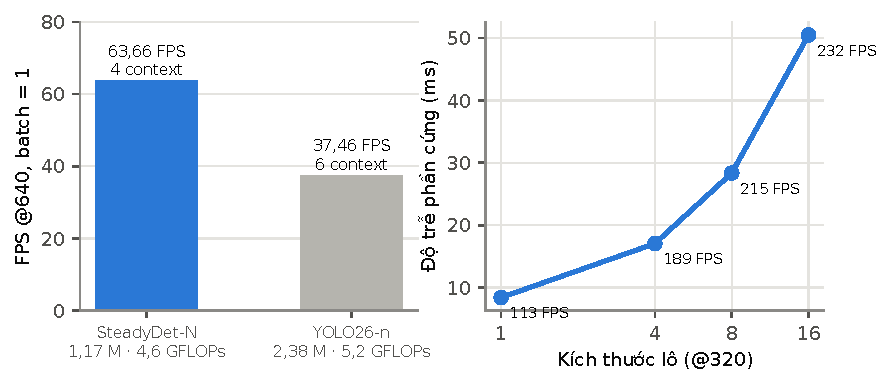
\includegraphics[width=\textwidth]{hailo.pdf}
\caption{Trái: tốc độ SteadyDet-N và YOLO26-n trên cùng Hailo-8L. Phải: độ trễ phần cứng tăng theo batch size dù thông lượng tăng}
\label{fig:hailo}
\end{figure}

\section{Độ trễ đầu-cuối với camera thật}
\label{sec:e2e}

\subsection{Hai lỗi phía camera làm hệ thống kẹt ở 15 khung hình/giây}

Lần đo đầu tiên với camera thật chỉ đạt 15,4 khung hình/giây, trong khi NPU mới dùng khoảng 17,8\,ms trong ngân sách 33,3\,ms. Đo tách riêng từng chặng cho thấy nút cổ chai không nằm ở mô hình mà ở camera, do hai lỗi độc lập nhân với nhau (Hình~\ref{fig:camera}):
\begin{enumerate}
\item \textbf{Bộ đệm camera bằng 1.} Tham số \texttt{CAP\_PROP\_BUFFERSIZE = 1} vốn được đặt để luôn lấy khung mới nhất, nhưng khi ứng dụng đang giữ bộ đệm duy nhất, trình điều khiển không có chỗ ghi khung kế tiếp nên bỏ luôn khung đó: 30 khung/giây thành đúng 15,0. Tăng lên 2 cho 30,0 khung/giây, còn độ cũ của khung đo được chỉ trung vị 15,7\,ms, bằng nửa chu kỳ khung như lý thuyết.
\item \textbf{Tự phơi sáng tự hạ tốc độ khung.} Khi thiếu sáng, firmware của camera kéo dài thời gian phơi sáng quá 1/30\,s và tự giảm tốc độ khung (đo được 24,9 khung/giây ở thời gian phơi sáng 1/25\,s). Cờ UVC dùng để cấm hành vi này bị firmware bỏ qua. Đề tài giải quyết bằng cách khoá phơi sáng thủ công và tự viết bộ điều chỉnh độ sáng bằng phần mềm (SoftAE) có trần thời gian phơi sáng cứng: đo độ sáng trung bình mỗi khung rồi điều chỉnh thời gian phơi sáng và độ khuếch đại. Kết quả: độ sáng bám giá trị đặt, tốc độ khung giữ 30,1.
\end{enumerate}
Sau khi sửa cả hai, tốc độ tăng từ 11,1 lên 30,0 khung hình/giây mà không thay đổi dòng nào của mô hình. Tần số lưới điện của camera cũng được đặt về 50\,Hz theo điện lưới Việt Nam để tránh sọc nhấp nháy dưới đèn huỳnh quang.

\begin{figure}[H]
\centering
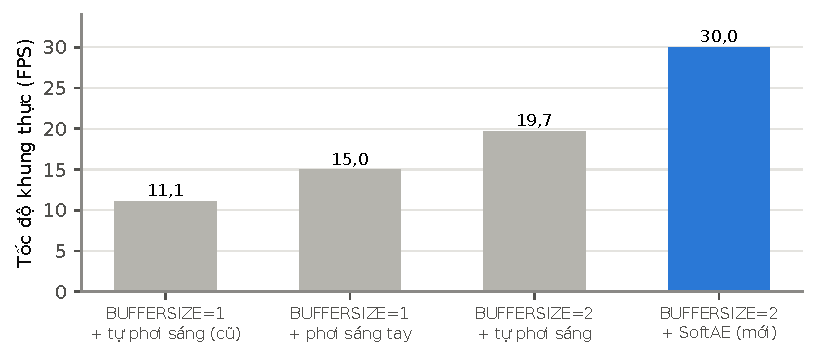
\includegraphics[width=0.9\textwidth]{camera_fps.pdf}
\caption{Tốc độ khung thực tế của chuỗi xử lý với bốn cấu hình camera}
\label{fig:camera}
\end{figure}

\subsection{Phân tích độ trễ từng chặng}

Chuỗi xử lý được đo liên tục trong 2 phút với camera thật ở $640\times640$ (3.594 khung). Bảng~\ref{tab:e2e} và Hình~\ref{fig:dotre} trình bày kết quả.

\begin{table}[H]
\centering
\caption{Độ trễ từng chặng của chuỗi xử lý trên Raspberry Pi~5 + Hailo-8L (ms), 3.594 khung}
\label{tab:e2e}
\small
\renewcommand{\arraystretch}{1.15}
\begin{tabular}{@{}lccccc@{}}
\toprule
\textbf{Chặng} & \textbf{Trung bình} & \textbf{p50} & \textbf{p95} & \textbf{p99} & \textbf{Lớn nhất}\\
\midrule
Chờ và đọc khung camera & 13,85 & 12,47 & 16,52 & 16,91 & 226,64\\
Tiền xử lý (letterbox, đổi kênh màu) & 0,98 & 0,99 & 1,02 & 1,04 & 1,67\\
Suy luận trên NPU & 17,73 & 17,72 & 17,83 & 17,89 & 18,09\\
Giải mã + NMS & 0,84 & 0,84 & 0,87 & 0,88 & 7,57\\
\midrule
\textbf{Tổng} & \textbf{33,39} & \textbf{32,04} & \textbf{36,08} & \textbf{36,15} & 246,76\\
\bottomrule
\end{tabular}
\end{table}

\begin{figure}[H]
\centering
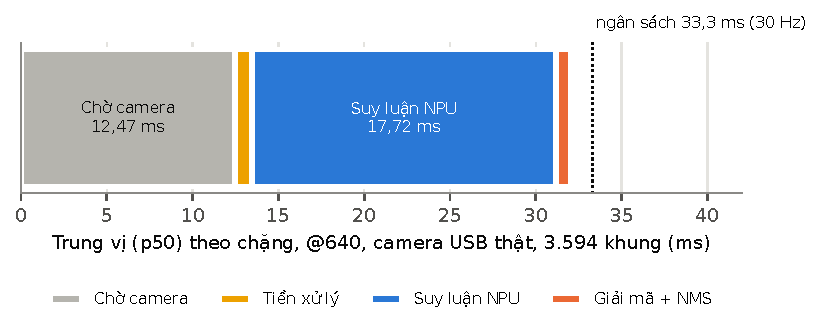
\includegraphics[width=\textwidth]{do_tre.pdf}
\caption{Phân bổ độ trễ trung vị theo chặng so với ngân sách 33,3\,ms của vòng lặp 30\,Hz}
\label{fig:dotre}
\end{figure}

Ba chặng tính toán (tiền xử lý, suy luận, giải mã) cộng lại chỉ 19,55\,ms trong ngân sách 33,3\,ms, tức hệ số sử dụng 59\%; phần còn lại là thời gian chờ camera. Hệ thống vì thế \textbf{bị giới hạn bởi camera chứ không bởi mô hình}: camera C270 tối đa 30 khung/giây, và muốn nhanh hơn thì phải đổi camera. Tốc độ khung giữ 29,9 ở phút đầu và 30,0 ở phút cuối, nhiệt độ SoC 48,5\,°C, cờ giảm xung nhiệt bằng 0 trong suốt thời gian đo. Khoảng dao động của chặng suy luận rất hẹp (p50 17,72\,ms, p99 17,89\,ms), điều quan trọng với bộ điều khiển vì nó phụ thuộc vào khung chậm nhất chứ không phải khung trung bình. Giá trị lớn nhất (246,76\,ms) chỉ là các khung cá biệt ở chặng camera, không ảnh hưởng tới p99.

Phép đo đầu-cuối này được thực hiện với bản HEF $640\times640$ cùng kiến trúc trước khi tệp triển khai cuối cùng được biên dịch; bản triển khai có độ trễ suy luận trung vị 17,32\,ms, tương đương, nên kết luận về ngân sách thời gian vẫn giữ nguyên.

\section{Kết luận chương}

SteadyDet-N đã được đưa lên Raspberry Pi~5 + Hailo-8L thành công. Mô hình INT8 đạt AP@0,5 = 0,917 và F1 = 0,880 trên dữ liệu bay thật ở ngưỡng tin cậy 0,25; tổn thất lượng tử hoá đáng kể với người rất nhỏ nhưng không đáng kể với người ở độ cao bay thực tế. Trên NPU, mô hình chạy nhanh hơn YOLO26-n 1,70 lần nhờ cần ít context hơn. Toàn bộ chuỗi camera -- suy luận -- hậu xử lý đạt 30 khung hình/giây ổn định, với các chặng tính toán chỉ chiếm 59\% ngân sách thời gian. Hai lỗi phía camera được phát hiện và sửa nhờ đo từng chặng, cho thấy tầm quan trọng của việc đo trước khi tối ưu.

% =====================================================================
%  CHƯƠNG 6. HỆ THỐNG ĐIỀU KHIỂN BÁM NGƯỜI
%  Mã nguồn: follow_drone/ (main.py, follow/*.py, config.yaml)
%  Số đo: runs/control_rate_2026-08-27.md, runs/mavlink_check_2026-08-27.md
% =====================================================================
\chapter{Hệ thống điều khiển máy bay bám theo người}
\label{chap:dieukhien}

Chương này trình bày chương trình máy tính điều khiển máy bay tự động đi theo người, tương ứng nội dung thứ ba của thuyết minh. Chương trình chạy trên Raspberry Pi~5, nhận kết quả phát hiện từ Chương~\ref{chap:trienkhai}, và gửi lệnh vận tốc tới bộ điều khiển bay ArduPilot. Thiết kế tuân theo một nguyên tắc xuyên suốt: phần mềm chỉ \textit{đề xuất} vận tốc trong một chế độ bay mà người lái đã chủ động giao quyền; mọi quyền quyết định chế độ bay thuộc về người lái.

\section{Kiến trúc tổng thể}

\begin{figure}[H]
\centering
\resizebox{\textwidth}{!}{% Kiến trúc tổng thể hệ thống UAV bám người
\begin{tikzpicture}[
  font=\footnotesize, >={Stealth[length=2mm]},
  m/.style={draw=black!60, rounded corners=2pt, align=center, minimum height=11mm, text width=2.6cm, inner sep=2pt, fill=white},
  pi/.style={m, fill=xanh!12},
  hw/.style={m, fill=black!6},
  fc/.style={m, fill=cam!14},
  lb/.style={font=\scriptsize, fill=white, inner sep=1pt}
]
% hàng 1: nhận thức
\node[hw] (cam) at (0,0) {Camera C270\\30 khung/giây};
\node[pi] (det) at (3.6,0) {Phát hiện người\\SteadyDet-N INT8};
\node[hw] (npu) at (3.6,1.9) {NPU Hailo-8L};
\node[pi] (trk) at (7.2,0) {Theo vết\\OC-SORT};
\node[pi] (sel) at (10.8,0) {Chọn \& khoá\\mục tiêu};
% hàng 2: điều khiển
\node[pi] (dist) at (10.8,-2.2) {Ước lượng khoảng cách\\pinhole + Kalman};
\node[pi] (servo) at (7.2,-2.2) {Servo thị giác\\3 bộ PID};
\node[pi] (safe) at (3.6,-2.2) {Lớp an toàn\\giới hạn + thang mất MT};
\node[pi] (mav) at (0,-2.2) {MAVLink client\\30\,Hz, chỉ khi GUIDED};
% hàng 3: phần cứng bay + người
\node[fc] (px) at (0,-4.8) {Pixhawk 6C\\ArduPilot};
\node[hw] (mot) at (3.6,-4.8) {Bộ điều tốc\\+ động cơ};
\node[hw, text width=3.0cm] (web) at (7.2,-4.8) {Bảng giám sát web\\(laptop, điện thoại)};
\node[hw] (rc) at (10.8,-4.8) {Tay điều khiển RC\\(người lái)};

\draw[->] (cam) -- (det);
\draw[<->] (det) -- (npu);
\draw[->] (det) -- (trk);
\draw[->] (trk) -- (sel);
\draw[->] (sel) -- (dist);
\draw[->] (dist) -- (servo);
\draw[->] (servo) -- (safe);
\draw[->] (safe) -- (mav);
\draw[<->] (mav) -- node[lb,right]{USB, MAVLink v2} (px);
\draw[->] (px) -- (mot);
\draw[->, dashed] (servo.south) ++(-0.4,0) -- ++(0,-1.45) node[lb,pos=0.5,left]{hình + trạng thái} ;
\draw[<-, dashed] ($(web.north)+(0.4,0)$) -- node[lb,right]{nút đổi mục tiêu} ($(servo.south)+(0.4,0)$);
\draw[->, thick, draw=cam] (rc.south) -- ++(0,-0.55) -| node[lb,pos=0.25,below]{gạt công tắc chế độ bay (luôn ưu tiên)} (px.south);

\begin{scope}[on background layer]
\node[draw=black!45, dashed, rounded corners=4pt, inner sep=7pt, fit=(det)(npu)(trk)(sel)(dist)(servo)(safe)(mav),
      label={[font=\footnotesize\bfseries, anchor=north east]north east:{Raspberry Pi 5 — chương trình \texttt{main.py}}}] {};
\end{scope}
\end{tikzpicture}
}
\caption{Kiến trúc tổng thể hệ thống. Toàn bộ khối xử lý nằm trên Raspberry Pi~5; bảng giám sát chỉ đọc (trừ nút đổi mục tiêu); tay điều khiển RC luôn có quyền ưu tiên cao nhất}
\label{fig:hethong}
\end{figure}

Hình~\ref{fig:hethong} mô tả luồng dữ liệu. Chương trình \texttt{main.py} gồm các mô-đun: \texttt{camera.py} (luồng đọc camera riêng, luôn trả khung mới nhất), \texttt{detector\_hailo.py} (suy luận trên NPU và hậu xử lý), \texttt{ocsort.py} (theo vết), \texttt{target\_selector.py} (chọn và khoá mục tiêu), \texttt{distance.py} (ước lượng khoảng cách), \texttt{visual\_servo.py} và \texttt{pid.py} (tính vận tốc), \texttt{safety.py} (lớp an toàn), \texttt{mavlink\_client.py} (giao tiếp với bộ điều khiển bay) và \texttt{dashboard.py} (bảng giám sát web). Mọi tham số được đặt trong một tệp cấu hình \texttt{config.yaml} duy nhất.

Bộ điều khiển bay Pixhawk~6C nối với Pi qua cổng USB. Vì cổng nối tiếp này chỉ cho phép một tiến trình mở, đề tài viết thêm công cụ \texttt{mavmux.py}: một tiến trình giữ cổng USB và phát lại nguyên từng byte ra hai cổng UDP nội bộ (14550 cho vòng bám, 14551 dự phòng cho trạm mặt đất). Kiểm tra với hai chương trình đồng thời cho thấy mỗi bên nhận khoảng 100 gói tin/giây với đầy đủ thông tin trạng thái.

\section{Vòng lặp điều khiển}

Vòng lặp chính chạy với chu kỳ 33,3\,ms (30\,Hz) và thực hiện tuần tự mười bước như Hình~\ref{fig:vongdieukhien}.

\begin{figure}[H]
\centering
\resizebox{!}{0.62\textheight}{% Lưu đồ một vòng lặp điều khiển 30 Hz
\begin{tikzpicture}[
  font=\footnotesize, >={Stealth[length=2mm]},
  st/.style={draw=black!60, rounded corners=2pt, align=center, minimum height=8mm, text width=5.2cm, inner sep=2pt, fill=white},
  sm/.style={st, text width=3.6cm},
  io/.style={st, fill=xanh!12},
  dc/.style={diamond, draw=black!60, aspect=2.8, align=center, inner sep=0pt, fill=cam!10, font=\scriptsize, text width=2.4cm},
  tm/.style={st, rounded corners=9pt, fill=black!8}
]
\node[tm] (s) at (0,0) {Bắt đầu vòng lặp (chu kỳ 33,3\,ms)};
\node[io] (a) at (0,-1.1) {1. Lấy khung mới nhất từ camera};
\node[st] (b) at (0,-2.2) {2. Phát hiện người trên NPU (ngưỡng 0,25; NMS)};
\node[st] (c) at (0,-3.3) {3. Cập nhật bộ theo vết OC-SORT};
\node[st] (d) at (0,-4.4) {4. Chọn/khoá mục tiêu (xử lý nút đổi mục tiêu)};
\node[io] (e) at (0,-5.5) {5. Đọc trạng thái máy bay qua MAVLink};
\node[dc] (f) at (0,-6.9) {Có mục tiêu?};
\node[sm] (g) at (-3.4,-8.4) {6. Khoảng cách pinhole + Kalman $\rightarrow$ 3 PID $\rightarrow$ giới hạn an toàn};
\node[sm] (h) at (3.4,-8.4) {Đặt lại các bộ PID};
\node[st] (i) at (0,-9.9) {7. Cập nhật thang mất mục tiêu\\8. Kiểm tra sức khoẻ hệ thống};
\node[dc] (j) at (0,-11.5) {Đang ở GUIDED?};
\node[sm, fill=xanh!12] (k) at (-3.4,-13.0) {9. Gửi vận tốc: FOLLOW / COAST ($\times0{,}5$) / HOVER (0)};
\node[sm] (l) at (3.4,-13.0) {Không gửi lệnh (người lái đang giữ quyền)};
\node[st] (m) at (0,-14.5) {10. Ghi log CSV, cập nhật bảng giám sát};
\foreach \x/\y in {s/a,a/b,b/c,c/d,d/e,e/f,i/j} \draw[->] (\x) -- (\y);
\draw[->] (f.west) -| node[pos=0.25,above,font=\scriptsize]{có} (g.north);
\draw[->] (f.east) -| node[pos=0.25,above,font=\scriptsize]{không} (h.north);
\draw[->] (g.south) |- (i.west);
\draw[->] (h.south) |- (i.east);
\draw[->] (j.west) -| node[pos=0.25,above,font=\scriptsize]{có} (k.north);
\draw[->] (j.east) -| node[pos=0.25,above,font=\scriptsize]{không} (l.north);
\draw[->] (k.south) |- (m.west);
\draw[->] (l.south) |- (m.east);
\draw[->] (m.south) -- ++(0,-0.4) -- ++(6.0,0) |- (s.east);
\end{tikzpicture}
}
\caption{Lưu đồ một vòng lặp điều khiển 30\,Hz trong \texttt{main.py}}
\label{fig:vongdieukhien}
\end{figure}

Có ba điểm đáng chú ý trong lưu đồ. \textit{Thứ nhất}, khi không có mục tiêu, các bộ PID được đặt lại để thành phần tích phân không tích luỹ sai số cũ. \textit{Thứ hai}, lệnh vận tốc chỉ được gửi khi máy bay đang ở chế độ GUIDED; ở mọi chế độ khác chương trình im lặng và in một dòng thông báo. \textit{Thứ ba}, bước ghi nhật ký và cập nhật bảng giám sát dùng lại chính khung hình và kết quả phát hiện của vòng lặp, không tốn thêm lượt suy luận nào; điều này bắt buộc vì NPU Hailo chỉ cho phép một tiến trình sử dụng.

\section{Theo vết đa đối tượng}

Kết quả phát hiện ở từng khung độc lập với nhau, trong khi bộ điều khiển cần biết người \textit{nào} đang được bám qua thời gian. Đề tài dùng OC-SORT~\cite{cao2023ocsort} vì ba lý do: không cần mạng trích đặc trưng ngoại hình nên chạy nhẹ trên CPU; xử lý tốt trường hợp mất phát hiện vài khung nhờ hiệu chỉnh dựa trên quan sát; và có kết quả tốt trên các benchmark theo vết người. Mỗi đối tượng được biểu diễn bằng một bộ lọc Kalman với trạng thái gồm tâm hộp, diện tích, tỷ lệ khung hình và vận tốc tương ứng. Phát hiện mới được ghép với dự đoán bằng thuật toán Hungary trên ma trận IoU.

\begin{table}[H]
\centering
\caption{Tham số bộ theo vết OC-SORT}
\label{tab:ocsort}
\small
\renewcommand{\arraystretch}{1.15}
\begin{tabularx}{\textwidth}{@{}lc>{\raggedright\arraybackslash}X@{}}
\toprule
\textbf{Tham số} & \textbf{Giá trị} & \textbf{Ý nghĩa và lý do chọn}\\
\midrule
\texttt{max\_age} & 45 khung & Giữ vết sống 1,5\,s khi mất phát hiện. Giá trị ban đầu 90 (3\,s) quá dài: bám theo dự đoán 3 giây thì người đã kịp đổi hướng\\
\texttt{min\_hits} & 3 & Cần 3 lần phát hiện liên tiếp mới xác nhận vết, loại bỏ hộp sai thoáng qua\\
\texttt{iou\_threshold} & 0,3 & Ngưỡng IoU tối thiểu để ghép phát hiện với vết\\
\texttt{delta\_t} & 3 & Số khung nhìn lại để ước lượng hướng chuyển động\\
\bottomrule
\end{tabularx}
\end{table}

Trước khi đưa vào bộ theo vết, phát hiện được lọc thêm hai điều kiện đơn giản: bỏ các hộp có diện tích dưới 200 điểm ảnh vuông và các hộp có tỷ lệ cạnh lớn hơn 6, vì người ở độ cao 3--6\,m luôn lớn hơn và có hình dạng hợp lý hơn thế.

\section{Chọn và khoá mục tiêu}

Khi có nhiều người trong khung hình, hệ thống phải chọn một người và bám ổn định người đó. Chiến lược mặc định chọn hộp có diện tích lớn nhất (thường là người gần nhất) ở lần đầu, rồi \textbf{khoá vào mã định danh} của vết đó; sau khi khoá, hệ thống bám đúng người này kể cả khi có người khác xuất hiện gần hơn.

Một khó khăn thực tế là OC-SORT cấp mã định danh \textit{mới} cho người rời khung rồi quay lại, vì nó không có cơ chế nhận dạng lại theo ngoại hình. Nếu không xử lý, sau khi mất mục tiêu, hệ thống có thể khoá nhầm vào một người lạ đứng gần hơn. Đề tài giải quyết bằng một cơ chế liên tục không gian đơn giản:
\begin{enumerate}
\item Khi mục tiêu biến mất, khoá được giữ thêm $3$\,s (\texttt{lost\_grace\_s}), bằng đúng pha máy bay còn bám theo dự đoán.
\item Sau khi nhả khoá, trong $5$\,s tiếp theo (\texttt{reacquire\_s}) hệ thống \textit{chỉ} chấp nhận một vết có tâm cách vị trí cuối của mục tiêu cũ không quá 25\% đường chéo khung hình và diện tích chênh không quá 2 lần. Người cũ quay lại chỗ cũ, dù mang mã mới, được bám lại ngay; người lạ không bị ``vồ'' nhầm.
\item Hết cửa sổ tìm lại, hệ thống mới chọn mục tiêu mới theo chiến lược (có thể tắt để chờ người vận hành bằng \texttt{auto\_relock: false}).
\end{enumerate}
Hai ngưỡng ở bước 2 được đặt chặt có chủ ý: thà không nhận ra còn hơn bám nhầm người. Cơ chế này đúng khi người quay lại gần chỗ cũ và có thể sai khi hai người đổi chỗ cho nhau, vì vậy bảng giám sát có nút \textbf{Đổi mục tiêu} cho người vận hành bỏ khoá và chọn lại ngay lập tức. Toàn bộ các tình huống trên được kiểm tra bằng bộ kiểm thử tự động \texttt{test\_target\_selector.py} gồm 14 phép kiểm tra (Chương~\ref{chap:tichhop}).

\begin{table}[H]
\centering
\caption{Diễn biến hành vi khi mất mục tiêu (tính từ lần cuối nhìn thấy)}
\label{tab:matmuctieu}
\small
\renewcommand{\arraystretch}{1.15}
\begin{tabularx}{\textwidth}{@{}l>{\raggedright\arraybackslash}X>{\raggedright\arraybackslash}X@{}}
\toprule
\textbf{Thời gian} & \textbf{Bám ai (bộ chọn mục tiêu)} & \textbf{Máy bay làm gì (lớp an toàn)}\\
\midrule
0 -- 1,5\,s & OC-SORT giữ vết bằng dự đoán Kalman & Tiếp tục bám\\
1,5 -- 4,5\,s & Vẫn giữ khoá mục tiêu & COAST: vận tốc giảm một nửa (từ 0 tới 3\,s mất mục tiêu)\\
4,5 -- 9,5\,s & Chỉ tìm lại đúng người cũ & HOVER: vận tốc bằng 0, đứng yên\\
sau 9,5\,s & Cho phép chọn người khác & HOVER cho tới khi thấy lại mục tiêu hoặc người lái lấy lại quyền\\
\bottomrule
\end{tabularx}
\end{table}

\section{Ước lượng khoảng cách}

Khoảng cách tới người được ước lượng từ chiều cao bounding box theo mô hình lỗ kim, phương trình~(\ref{eq:distance}), với chiều cao người giả định $H_r = 1{,}7$\,m. Tệp cấu hình hiện đặt tiêu cự $f_x = f_y = 700$ điểm ảnh và tâm ảnh $(320, 240)$ cho độ phân giải $640\times480$; hệ thống kèm công cụ \texttt{calibrate\_camera.py} để hiệu chuẩn lại bằng bàn cờ theo phương pháp của Zhang~\cite{zhang2000calibration}. Độ phân giải camera được giữ ở $640\times480$ vì hai lý do: các tham số nội của camera gắn với độ phân giải này (chuyển sang 16:9 làm thay đổi cả góc nhìn chứ không chỉ tỷ lệ), và mô hình vốn đưa ảnh về 640 điểm ảnh nên độ phân giải cao hơn không thêm điểm ảnh nào trên người mà chỉ tốn CPU giải nén.

Kết quả đo được loại bỏ khi hộp thấp hơn 20 điểm ảnh hoặc khoảng cách nằm ngoài khoảng 0,5--30\,m. Vì sai số tăng theo bình phương khoảng cách, phương sai đo được mô hình hoá là $\sigma^2 = \max\big(0{,}1,\ (2d^2/f_y)^2\big)$, ứng với sai số chiều cao hộp khoảng 2 điểm ảnh. Giá trị đo được làm mượt bằng bộ lọc Kalman một chiều với trạng thái $[d,\ \dot d]^\top$, mô hình vận tốc không đổi; phương sai đo thay đổi theo từng lần đo nên các phép đo ở xa (kém tin cậy) tự động được tin ít hơn.

\section{Servo thị giác và bộ điều khiển PID}

Đề tài dùng cách tiếp cận servo thị giác lai~\cite{chaumette2006visual}: kênh quay hướng dùng sai số trực tiếp trên ảnh, kênh tiến lùi dùng khoảng cách ước lượng, kênh độ cao dùng độ cao đo từ bộ điều khiển bay. Ba bộ điều khiển PID độc lập theo phương trình~(\ref{eq:pid}) sinh ra vận tốc trong hệ toạ độ thân máy bay; vận tốc ngang bằng 0 vì chuyển động sang ngang được thực hiện bằng cách quay hướng.

\begin{itemize}
\item \textbf{Kênh tiến lùi:} sai số là khoảng cách đã làm mượt trừ khoảng cách đặt 5\,m. Người ở xa hơn 5\,m thì máy bay tiến tới, gần hơn thì lùi lại. Khi không có khoảng cách tin cậy, vận tốc tiến bằng 0.
\item \textbf{Kênh quay hướng:} sai số góc $e_\psi = (u_c - W/2)/f_x$ (radian), với $u_c$ là hoành độ tâm hộp và $W$ là bề rộng ảnh. Người lệch phải thì máy bay quay phải. Kênh này không dùng thành phần tích phân: sai số góc tự về 0 khi máy bay quay tới, còn tích phân chỉ tích luỹ rồi gây vọt lố mỗi khi mục tiêu ra khỏi khung.
\item \textbf{Kênh độ cao:} giữ độ cao 5\,m so với mặt đất; đầu ra được đổi dấu khi gửi vì trục $z$ của hệ NED hướng xuống.
\end{itemize}

\begin{table}[H]
\centering
\caption{Tham số ba bộ điều khiển PID}
\label{tab:pid}
\small
\renewcommand{\arraystretch}{1.15}
\begin{tabular}{@{}lcccccc@{}}
\toprule
\textbf{Kênh} & \textbf{Giá trị đặt} & \textbf{$K_p$} & \textbf{$K_i$} & \textbf{$K_d$} & \textbf{Giới hạn đầu ra} & \textbf{Giới hạn tích phân}\\
\midrule
Tiến lùi & 5,0\,m & 0,5 & 0,05 & 0,1 & $\pm$3,0\,m/s & $\pm$2,0\\
Quay hướng & 0\,rad & 2,0 & 0 & 0,3 & $\pm$1,5\,rad/s & --\\
Độ cao & 5,0\,m & 0,8 & 0,1 & 0,2 & $\pm$2,0\,m/s & $\pm$1,0\\
\bottomrule
\end{tabular}
\end{table}

Bước thời gian được đo thực tế giữa hai lần gọi thay vì giả định cố định. Nếu khoảng cách giữa hai lần gọi vượt 1\,s (ví dụ sau khi mất mục tiêu lâu), bộ điều khiển tự đặt lại để tránh thành phần vi phân và tích phân nhận giá trị bất thường. Vận tốc trong hệ thân được chuyển sang hệ NED bằng góc hướng hiện tại $\psi$ của máy bay:
\begin{equation}
v_N = v_x \cos\psi - v_y \sin\psi, \qquad v_E = v_x \sin\psi + v_y \cos\psi,
\end{equation}
rồi gửi bằng thông điệp \texttt{SET\_POSITION\_TARGET\_LOCAL\_NED} với mặt nạ chỉ dùng ba thành phần vận tốc và tốc độ quay hướng.

\section{Lớp an toàn}
\label{sec:antoan}

An toàn được thiết kế nhiều lớp, mỗi lớp độc lập với các lớp còn lại.

\textbf{Giới hạn lệnh.} Vận tốc ngang bị chặn $\pm$5\,m/s, vận tốc đứng $\pm$2\,m/s, tốc độ quay hướng $\pm$1,0\,rad/s (57\,°/s, thấp hơn giới hạn 60\,°/s của bộ điều khiển bay để lệnh không bị cắt). Khi người ở gần hơn 3\,m, máy bay bị buộc lùi với vận tốc ít nhất 0,5\,m/s; khi xa hơn 15\,m, vận tốc tiến bị giới hạn 1\,m/s vì phát hiện ở xa kém tin cậy. Máy bay không được hạ thấp hơn 2\,m hay lên cao quá 25\,m so với mặt đất.

\textbf{Kiểm tra trước khi cất cánh.} Chương trình chỉ cất cánh khi GPS có định vị 3D với HDOP không quá 2,0, điện áp pin không dưới 14,8\,V (3,7\,V mỗi cell với pin 4S) và gói \texttt{HEARTBEAT} mới nhất cách không quá 2\,s.

\textbf{Kiểm tra trong khi bay.} Mỗi vòng lặp kiểm tra: mất \texttt{HEARTBEAT} quá 3\,s, mất định vị GPS, pin dưới 14,0\,V, độ cao vượt 1,5 lần giới hạn. Khi một điều kiện bị vi phạm, chương trình \textbf{ngừng gửi lệnh và thoát vòng bám, nhưng không đổi chế độ bay}. Bộ điều khiển bay tự dừng máy bay sau thời gian \texttt{GUID\_TIMEOUT} = 1\,s, còn người lái lấy lại quyền bằng công tắc chế độ.

\textbf{Thang mất mục tiêu.} Hình~\ref{fig:antoan} mô tả máy trạng thái. Khi mất mục tiêu dưới 3\,s (COAST), máy bay tiếp tục theo lệnh tính từ dự đoán với vận tốc giảm một nửa; sau 3\,s (HOVER), vận tốc bằng 0 và máy bay đứng yên cho tới khi thấy lại mục tiêu hoặc người lái chuyển chế độ. Thang \textit{không} leo thang sang LOITER hay RTL: chế độ RTL của ArduPilot trước tiên leo lên độ cao an toàn \texttt{RTL\_ALT} (mặc định 15\,m), một hành động bất ngờ với người lái nếu phần mềm tự kích hoạt, nên quyết định chuyển chế độ được dành cho người lái.

\begin{figure}[H]
\centering
\resizebox{0.85\textwidth}{!}{% Máy trạng thái thang mất mục tiêu
\begin{tikzpicture}[
  font=\footnotesize, >={Stealth[length=2mm]},
  s/.style={circle, draw=black!60, align=center, minimum size=19mm, inner sep=1pt, fill=white},
]
\node[s, fill=xanh!15] (F) {FOLLOW\\\scriptsize bám theo};
\node[s, fill=cam!12, right=3.2cm of F] (C) {COAST\\\scriptsize vận tốc $\times0{,}5$};
\node[s, fill=black!8, right=3.2cm of C] (H) {HOVER\\\scriptsize vận tốc 0};
\draw[->] (F) to[bend left=18] node[above,font=\scriptsize,align=center]{mất mục tiêu} (C);
\draw[->] (C) to[bend left=18] node[below,font=\scriptsize]{thấy lại} (F);
\draw[->] (C) -- node[above,font=\scriptsize,align=center]{mất $\ge$ 3\,s} (H);
\draw[->] (H) to[bend left=35] node[below,font=\scriptsize]{thấy lại mục tiêu} (F);
\draw[->] (H) edge[loop right] node[right,font=\scriptsize,align=left]{đứng yên đến khi\\người lái gạt\\công tắc chế độ} (H);
\end{tikzpicture}
}
\caption{Máy trạng thái của thang mất mục tiêu; phần mềm không bao giờ tự đổi chế độ bay}
\label{fig:antoan}
\end{figure}

\textbf{Người lái luôn giữ quyền.} Phần mềm chỉ gọi lệnh đổi chế độ bay ở đúng một chỗ: chuỗi cất cánh tự động khi người vận hành chủ động chạy chương trình ở chế độ bay thật. Mọi lệnh vận tốc chỉ được gửi khi máy bay đang ở GUIDED; gạt công tắc sang LOITER hay STABILIZE là phần mềm im lặng ngay lập tức. Nhấn Ctrl+C gửi vận tốc 0 rồi buông quyền, không tự quay về. Nguyên tắc này được khoá bằng bộ kiểm thử \texttt{test\_safety\_no\_mode\_change.py}, trong đó có phép kiểm tra quét mã nguồn \texttt{safety.py} để đảm bảo không còn lời gọi đổi chế độ nào.

\textbf{Tham số trên bộ điều khiển bay.} Khi kết nối lần đầu với Pixhawk~6C (ArduPilot Copter 4.7.0), nhóm tải đủ 1.038 tham số và phát hiện năm cấu hình không an toàn cần sửa trước khi bay tự động: bỏ qua toàn bộ kiểm tra trước khi arm (\texttt{ARMING\_SKIPCHK} = $-1$), ngưỡng pin yếu và pin nguy kịch bị đặt ngược nhau (10\,V và 14\,V), không có hành động khi pin yếu, không có bảo vệ khi mất máy tính đồng hành (\texttt{FS\_GCS\_ENABLE} = 0), và hàng rào địa lý đã cấu hình nhưng đang tắt. Bảng tham số khuyến nghị được trình bày ở Phụ lục~A. Một lưu ý quan trọng là ArduPilot 4.7 đã đổi tên và đơn vị nhiều tham số (ví dụ \texttt{WPNAV\_SPEED} tính bằng cm/s thành \texttt{WP\_SPD} tính bằng m/s); chép giá trị từ tài liệu cho phiên bản cũ sẽ sai tới 100 lần.

\section{Giao tiếp MAVLink và lựa chọn nhịp gửi lệnh}

\subsection{Kiểm tra liên lạc}

Kết nối được kiểm tra trực tiếp trên máy bay (không phải mô phỏng): Pixhawk~6C chạy ArduPilot Copter 4.7.0, MAVLink v2, nhận 94--100 gói tin/giây với 0 lỗi truyền. Các thông điệp cần cho bảng giám sát đều về đủ nhịp: \texttt{ATTITUDE}, \texttt{VFR\_HUD}, \texttt{GLOBAL\_POSITION\_INT} ở 10\,Hz; \texttt{SYS\_STATUS}, \texttt{GPS\_RAW\_INT} ở 5\,Hz; \texttt{VIBRATION}, \texttt{EKF\_STATUS\_REPORT}, \texttt{BATTERY\_STATUS} ở 3,1\,Hz. Mọi cảm biến ở trạng thái tốt, các phương sai EKF3 dưới 0,01 và mức rung nền 0,01--0,07\,m/s² khi chưa quay động cơ. Quá trình kiểm tra cũng phát hiện hai lỗi trong mã của nhóm: chương trình đọc trạng thái gửi yêu cầu nhịp thông điệp \textit{chậm hơn} nhịp mà ArduPilot đang tự phát (làm giảm \texttt{VFR\_HUD} từ 10 xuống 5\,Hz), và bảng bit trạng thái cảm biến gõ tay bị lệch khiến trạng thái sẵn sàng arm không bao giờ đọc được. Cả hai đã được sửa: chỉ yêu cầu những thông điệp chưa nhận được sau 3 giây lắng nghe, và sinh bảng bit trực tiếp từ định nghĩa của thư viện pymavlink.

\subsection{Chọn nhịp gửi lệnh 30\,Hz}

Nhịp gửi lệnh được chọn dựa trên số đo. Khứ hồi một lệnh từ Pi tới máy bay và nhận xác nhận có trung vị 4,75\,ms, p95 6,24\,ms, p99 7,73\,ms (120 mẫu), tức một chiều khoảng 2,4\,ms; gửi ở 50\,Hz không mất gói nào (200/200). Độ trễ từ lúc ánh sáng vào cảm biến tới lúc lệnh tới bộ điều khiển bay gồm độ trễ phát hiện (32,0\,ms), thời gian chờ tới lượt gửi và thời gian truyền (Bảng~\ref{tab:nhiplenh}, Hình~\ref{fig:nhiplenh}).

\begin{table}[H]
\centering
\caption{Ngân sách độ trễ từ ảnh tới lệnh theo nhịp gửi (ms)}
\label{tab:nhiplenh}
\small
\renewcommand{\arraystretch}{1.15}
\begin{tabular}{@{}lccccc@{}}
\toprule
\textbf{Nhịp gửi} & \textbf{Phát hiện} & \textbf{Chờ (TB / xấu nhất)} & \textbf{Truyền} & \textbf{Tổng TB} & \textbf{Tổng xấu nhất}\\
\midrule
10\,Hz & 32,0 & 50,0 / 100,0 & 2,4 & 84,4 & 138,4\\
20\,Hz & 32,0 & 25,0 / 50,0 & 2,4 & 59,4 & 88,4\\
\textbf{30\,Hz} & 32,0 & \textbf{16,7 / 33,3} & 2,4 & \textbf{51,1} & \textbf{71,7}\\
50\,Hz & 32,0 & 10,0 / 20,0 & 2,4 & 44,4 & 58,4\\
\bottomrule
\end{tabular}
\end{table}

\begin{figure}[H]
\centering
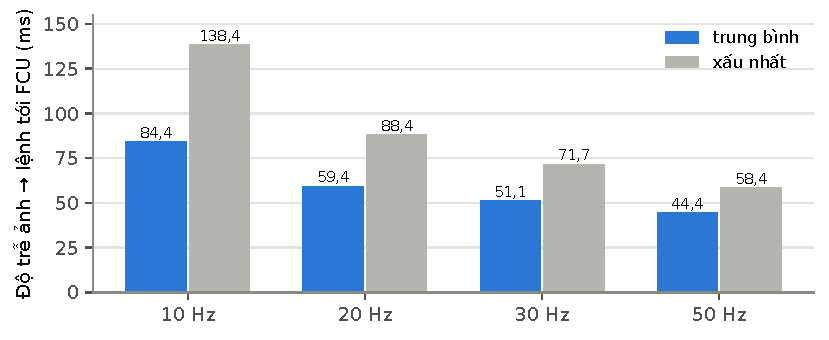
\includegraphics[width=0.9\textwidth]{nhip_lenh.pdf}
\caption{Độ trễ từ ảnh tới lệnh theo nhịp gửi}
\label{fig:nhiplenh}
\end{figure}

Ở 10\,Hz, mỗi phát hiện phải chờ trung bình 50\,ms mới được gửi đi: thêm 50\,ms trễ mà không đổi lấy lợi ích gì. Với người đi bộ 1,5\,m/s, 50\,ms tương ứng 7,5\,cm sai lệch, và trong vòng kín nó tích luỹ thành vọt lố. Ở 50\,Hz, vì bộ phát hiện chỉ sinh thông tin mới 30 lần mỗi giây, 20 trong 50 lệnh không mang phát hiện mới nào, trong khi chỉ lợi thêm 6,7\,ms. \textbf{Nhịp 30\,Hz khớp một-một với nhịp của bộ phát hiện}: mỗi lệnh mang đúng một phát hiện mới. Băng thông tương ứng khoảng 2\,KB/s, không đáng kể với đường USB. Nhịp này cũng nằm trong vùng hoạt động tốt mà các lập trình viên ArduPilot khuyến nghị cho chế độ GUIDED (trên 10\,Hz)~\cite{ardupilot}. Kèm theo đó, thời gian chờ lệnh của phần mềm và \texttt{GUID\_TIMEOUT} của máy bay được hạ từ 3\,s xuống 1\,s: ở 30\,Hz, 3\,s tương đương 90 lệnh bị mất trước khi máy bay chịu dừng.

\section{Bảng giám sát và ghi nhật ký}

Bảng giám sát là một trang web do chính \texttt{main.py} phục vụ ở cổng 8080, mở được trên laptop hoặc điện thoại cùng mạng WiFi mà không cần màn hình gắn vào Pi. Trang hiển thị video có vẽ hộp và mục tiêu đang khoá, chế độ bay, trạng thái arm, độ cao, pin, GPS, tư thế, mức rung thật ba trục, trạng thái vòng bám (FOLLOW/COAST/HOVER), khoảng cách ước lượng, bốn thành phần vận tốc đang gửi, độ trễ từng chặng, nhiệt độ SoC và trạng thái giảm xung nhiệt. Thao tác duy nhất trang cho phép là nút \textbf{Đổi mục tiêu}; trang không thể arm, đổi chế độ hay gửi vận tốc.

Mỗi vòng lặp ghi một dòng nhật ký CSV gồm thời gian, trạng thái an toàn, chế độ bay, vị trí và vận tốc máy bay, độ cao, pin, GPS, mã mục tiêu, bounding box, khoảng cách thô và đã làm mượt, lệnh vận tốc, cùng \textbf{mức rung ba trục, số lần bão hoà cảm biến gia tốc, số phát hiện và điểm tin cậy cao nhất}. Việc đặt mức rung đo thật và chất lượng phát hiện trên cùng một dòng, cùng một dấu thời gian là cơ sở để đối chiếu mô hình rung mô phỏng của Chương~\ref{chap:dulieu} với rung thật trong các chuyến bay tiếp theo.

\section{Kết luận chương}

Chương trình điều khiển bám người đã được xây dựng hoàn chỉnh: theo vết OC-SORT, khoá mục tiêu có cơ chế tìm lại người cũ, ước lượng khoảng cách pinhole có bộ lọc Kalman, ba bộ PID trong cấu trúc servo thị giác lai, lớp an toàn nhiều tầng với nguyên tắc người lái luôn giữ quyền chế độ bay, giao tiếp MAVLink 30\,Hz với độ trễ và băng thông được đo kiểm, bảng giám sát web và nhật ký bay có dữ liệu rung thật. Mọi tham số quan trọng đều được chọn dựa trên số đo và được ghi lại lý do trong tệp cấu hình.

% =====================================================================
%  CHƯƠNG 7. TÍCH HỢP VÀ KIỂM THỬ TOÀN HỆ THỐNG
%  Nguồn: follow_drone/RUNBOOK.md, follow_drone/tests/*, runs/*_2026-08-2x.md,
%         demo_flight/flight_deploy_v17.mp4
% =====================================================================
\chapter{Tích hợp và kiểm thử toàn hệ thống}
\label{chap:tichhop}

Chương này trình bày việc tích hợp mô hình, camera và bộ điều khiển bay thành một hệ thống, quy trình kiểm thử phân tầng, kết quả bay thử, kết quả chạy vòng bám người trên video bay thử, và đánh giá mức độ đạt được so với các mục tiêu trong thuyết minh.

\section{Cấu hình hệ thống tích hợp}

\begin{table}[H]
\centering
\caption{Các thành phần của hệ thống tích hợp}
\label{tab:phancung}
\small
\renewcommand{\arraystretch}{1.15}
\begin{tabularx}{\textwidth}{@{}l>{\raggedright\arraybackslash}p{4.6cm}>{\raggedright\arraybackslash}X@{}}
\toprule
\textbf{Thành phần} & \textbf{Thiết bị} & \textbf{Vai trò và cách kết nối}\\
\midrule
Bộ điều khiển bay & Holybro Pixhawk~6C, ArduPilot Copter 4.7.0 & Ổn định tư thế, giữ vị trí, thực thi vận tốc đặt ở chế độ GUIDED; nối Pi qua USB (MAVLink v2)\\
Máy tính đồng hành & Raspberry Pi~5 & Chạy toàn bộ phần mềm bám người; nguồn 5\,V cấp riêng, không lấy từ bộ điều khiển bay\\
Bộ tăng tốc & Hailo-8L (13 TOPS), M.2 PCIe & Suy luận SteadyDet-N INT8\\
Camera & Logitech C270 HD, USB & Nguồn ảnh $640\times480$, 30 khung/giây, phơi sáng do SoftAE điều khiển\\
Nguồn bay & Pin LiPo 4S (đầy 16,8\,V) & Ngưỡng cảnh báo 14,8\,V, nguy kịch 14,0\,V\\
Điều khiển tay & Bộ phát/thu RC & Người lái chọn chế độ bay, luôn có quyền ưu tiên\\
Giám sát & Laptop hoặc điện thoại, WiFi & Mở bảng giám sát tại \texttt{http://pi5.local:8080}\\
\bottomrule
\end{tabularx}
\end{table}

Phần mềm trên Pi dùng môi trường Python ảo kế thừa các thư viện hệ thống (HailoRT, OpenCV, NumPy) và chỉ cài thêm các gói còn thiếu. Pi được truy cập bằng tên miền cục bộ \texttt{pi5.local} thay vì địa chỉ IP cố định vì địa chỉ do DHCP cấp thay đổi theo ngày. Một kịch bản \texttt{run.sh} gom các lệnh vận hành: \texttt{check} (kiểm tra trước khi ra bãi), \texttt{mux} (chia cổng MAVLink), \texttt{stream} (phát video lên trình duyệt), \texttt{bench} (đo độ trễ), \texttt{record} (thu dữ liệu bay).

\section{Quy trình kiểm thử phân tầng}

Mỗi tầng chỉ được kiểm thử khi tầng dưới đã đạt, để khi có lỗi thì biết chính xác lỗi thuộc tầng nào.

\begin{table}[H]
\centering
\caption{Các tầng kiểm thử và kết quả}
\label{tab:tangkiemthu}
\small
\renewcommand{\arraystretch}{1.15}
\begin{tabularx}{\textwidth}{@{}c>{\raggedright\arraybackslash}p{3.8cm}>{\raggedright\arraybackslash}X>{\raggedright\arraybackslash}p{3.4cm}@{}}
\toprule
\textbf{Tầng} & \textbf{Nội dung} & \textbf{Cách kiểm thử} & \textbf{Kết quả}\\
\midrule
1 & Logic chọn mục tiêu và lớp an toàn & Kiểm thử tự động không cần phần cứng & 25/25 phép kiểm tra đạt\\
2 & Mô hình trên NPU & Đánh giá 548 ảnh VisDrone-val và 92 khung bay thật ngay trên Pi & AP@0,5 = 0,917; F1 = 0,880\\
3 & Camera + suy luận & Đo liên tục 2 phút với camera thật & 30,0 FPS, p99 36,15\,ms, 48,5\,°C\\
4 & Kiểm tra môi trường & \texttt{./run.sh check}: HailoRT, thư viện, HEF, camera, chạy thử mô hình, nhiệt, dung lượng đĩa, đồng bộ NTP & 10 OK / 0 lỗi\\
5 & Liên lạc với máy bay & Đọc trạng thái, gửi lệnh yêu cầu thông điệp và đo khứ hồi tới 50\,Hz & 94--100 gói/s, 0\% mất gói, p99 7,73\,ms\\
6 & Toàn bộ vòng bám không cất cánh & \texttt{main.py --no-fly}: chạy đủ camera, NPU, theo vết, chọn mục tiêu, PID, bảng giám sát nhưng chặn mọi lệnh & Vòng lặp đạt 29,9\,Hz; suy luận 19,93\,ms/khung\\
7 & Bay thử ngoài bãi & Bay thử, thu video từ máy bay; chạy vòng bám người trên video bay thử & Giữ mục tiêu 83,5\% thời gian (mục~\ref{sec:vongbam})\\
\bottomrule
\end{tabularx}
\end{table}

\section{Kiểm thử tự động}

Hai bộ kiểm thử được viết bằng Python thuần, chạy không cần NPU, camera hay máy bay, nên có thể chạy lại mỗi khi sửa mã.

\textbf{Bộ \texttt{test\_target\_selector.py} (14 phép kiểm tra)} mô phỏng các chuỗi vết theo thời gian và kiểm tra: khoá đúng mã định danh ban đầu; giữ mã cũ khi có người khác xuất hiện; trả về rỗng trong thời gian giữ khoá (1,0\,s, 2,0\,s, 2,9\,s) và trong cửa sổ tìm lại (4\,s); bám lại đúng người cũ khi người đó quay lại với mã mới (77); không chọn người lạ trong cửa sổ tìm lại kể cả ở mốc sát cuối cửa sổ; chọn người còn lại khi hết cửa sổ; với \texttt{auto\_relock} tắt thì không tự chọn và bật cờ chờ người vận hành; nút đổi mục tiêu chọn đúng người còn lại.

\textbf{Bộ \texttt{test\_safety\_no\_mode\_change.py} (11 phép kiểm tra)} kiểm tra: mất mục tiêu tới 120\,s thang chỉ ra COAST hoặc HOVER, không bao giờ ra LOITER hay RTL, và không có lời gọi đổi chế độ nào; khi kiểm tra sức khoẻ thất bại (mô phỏng mất GPS) thì phát hiện được lỗi nhưng không đổi chế độ; thấy lại mục tiêu sau 60\,s thì quay về FOLLOW; và quét mã nguồn \texttt{safety.py} để khẳng định không còn lời gọi \texttt{set\_mode}.
Cả hai bộ đều in ``TẤT CẢ ĐỀU ĐẠT'' với phiên bản mã hiện tại.

\section{Bay thử}
\label{sec:baythu}

\subsection{Chuyến bay thu dữ liệu và video thử nghiệm}

Chuyến bay ngày 21/07/2026 được thực hiện ở chế độ giữ vị trí, độ cao khoảng 6\,m, có một người đi bộ trong vùng quan sát. Video từ trạm mặt đất dài 158,8\,giây được dùng cho hai mục đích: xây dựng tập đánh giá flight\_val 92 khung (Chương~\ref{chap:dulieu}) và dựng video thử nghiệm của đề tài. Video bay thử (tệp \texttt{video\_bay\_thu.mp4} nộp kèm hồ sơ, 283\,giây) gồm hai phần: phần 1 dựng từ \texttt{demo\_flight/flight\_deploy\_v17.mp4}, hiển thị kết quả phát hiện của SteadyDet-N nhánh triển khai (ảnh vào 512, ngưỡng 0,3) trên từng khung; phần 2 là vòng bám người chạy trên cùng chuyến bay (mục~\ref{sec:vongbam}). Hình~\ref{fig:demokhung} trích ba khung từ video. Ở giây 15 và 45, mô hình khoanh đúng người đi bộ ở các vị trí khác nhau trong khung. Ở giây 80, người đang đi ra khỏi mép trái ảnh, chỉ còn một phần cơ thể, và mô hình bỏ sót người này đồng thời sinh một hộp sai nhỏ trên mặt đất. Đây là dạng lỗi điển hình mà các bộ lọc kích thước hộp, yêu cầu 3 lần phát hiện liên tiếp của OC-SORT và thang mất mục tiêu ở Chương~\ref{chap:dieukhien} được thiết kế để chịu đựng.

\begin{figure}[H]
\centering
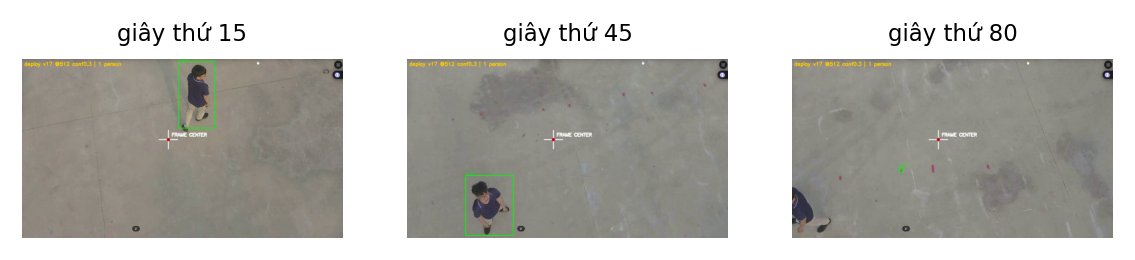
\includegraphics[width=\textwidth]{demo_khung.png}
\caption{Ba khung hình trích từ video bay thử (hộp xanh: phát hiện của SteadyDet-N; dấu thập: tâm khung hình). Giây 15 và 45: phát hiện đúng. Giây 80: người bị cắt ở mép trái bị bỏ sót và có một hộp sai nhỏ}
\label{fig:demokhung}
\end{figure}

Kết quả định lượng trên dữ liệu của chuyến bay này đã được trình bày ở Bảng~\ref{tab:baythat} và Bảng~\ref{tab:int8}. Đây cũng là chuyến bay cho thấy tầm quan trọng của dữ liệu cự ly gần: mô hình chỉ học VisDrone đạt AP@0,5 = 0,1435, còn mô hình có COCO-person đạt 0,7613 trên cùng dữ liệu.

\subsection{Vòng bám người trên video bay thử}
\label{sec:vongbam}

Để kiểm chứng toàn bộ chuỗi bám người trên dữ liệu thật của máy bay, video của chuyến bay 21/07/2026 được cho đi qua chính các mô-đun của chương trình \texttt{follow\_drone}: SteadyDet-N (ảnh vào 512, ngưỡng 0,30) $\rightarrow$ OC-SORT (tham số Bảng~\ref{tab:ocsort}) $\rightarrow$ bộ chọn và khoá mục tiêu $\rightarrow$ bộ PID quay hướng $\rightarrow$ thang trạng thái FOLLOW/COAST/HOVER. Công cụ \texttt{replay\_follow.py} xử lý lần lượt 3.961 khung (132\,giây, 30 khung/giây), ghi trạng thái, mã mục tiêu, sai số hướng và lệnh quay hướng của từng khung vào nhật ký CSV, đồng thời vẽ kết quả thành phần thứ hai của video bay thử. Vì phạm vi đề tài là bám một người, thời gian giữ khoá và cửa sổ tìm lại được đặt 1,5\,s và 1,0\,s; các biểu tượng giao diện của trạm mặt đất vẽ đè lên video được loại khỏi vùng xét.

\begin{figure}[H]
\centering
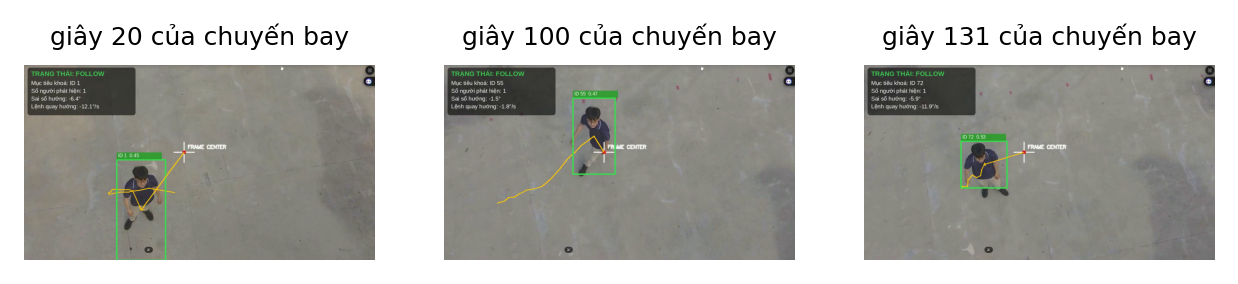
\includegraphics[width=\textwidth]{vongbam_khung.png}
\caption{Vòng bám người trên video bay thử: hộp xanh lá là mục tiêu đang khoá kèm mã định danh, mũi tên nối tâm khung hình với mục tiêu, vệt vàng là quỹ đạo; bảng góc trái hiển thị trạng thái, sai số hướng và lệnh quay hướng tính được}
\label{fig:vongbam}
\end{figure}

\begin{table}[H]
\centering
\caption{Kết quả vòng bám người trên video bay thử 21/07/2026 (3.961 khung)}
\label{tab:vongbam}
\small
\renewcommand{\arraystretch}{1.15}
\begin{tabular}{@{}lc@{}}
\toprule
\textbf{Chỉ số} & \textbf{Giá trị}\\
\midrule
Tỷ lệ khung ở trạng thái FOLLOW (có mục tiêu khoá và lệnh bám) & 40,5\%\\
Tỷ lệ khung giữ được mục tiêu (FOLLOW hoặc COAST) & 83,5\%\\
Đoạn giữ mục tiêu liên tục dài nhất & 25,4\,s\\
Đoạn FOLLOW liên tục dài nhất & 9,6\,s\\
Sai số hướng tới mục tiêu khi FOLLOW: trung vị / phân vị 90 & 5,5$^\circ$ / 13,5$^\circ$\\
\bottomrule
\end{tabular}
\end{table}

Kết quả cho thấy chuỗi xử lý khoá được người đi bộ và giữ khoá qua các khung mất phát hiện ngắn: khi mô hình bỏ sót người vài khung, trạng thái chuyển sang COAST với hộp dự đoán của OC-SORT rồi quay lại FOLLOW ngay khi phát hiện trở lại, nên máy bay giữ được mục tiêu trong 83,5\% thời gian. Sai số hướng trung vị 5,5$^\circ$ cho thấy người luôn nằm gần trục quang học khi đang bám. Phần thời gian HOVER tương ứng các đoạn người đi ra khỏi vùng nhìn của camera trong chuyến bay. Tỷ lệ FOLLOW còn bị giới hạn bởi các khung bỏ sót phát hiện (người ở rìa ảnh, bị cắt một phần), cho thấy việc tăng recall của mô hình trên dữ liệu bay thấp là hướng cải thiện trực tiếp nhất.

\subsection{Quy trình bay bám tự động}

Dựa trên kết quả các tầng kiểm thử, đề tài xây dựng quy trình vận hành năm bước (chi tiết ở Phụ lục~C): (0) sửa các tham số an toàn trên bộ điều khiển bay bằng Mission Planner; (1) chạy \texttt{./run.sh check} trên Pi; (2) ngoài bãi, chạy bộ chia cổng MAVLink và chương trình bám; (3) kiểm tra năm chỉ số trên bảng giám sát trước khi arm (sẵn sàng arm, GPS $\ge$ 8 vệ tinh và HDOP < 2,0, rung < 30\,m/s² và không bão hoà, pin > 15,5\,V, nhiệt độ < 70\,°C); (4) giao quyền: cất cánh ở LOITER bằng tay lên khoảng 5\,m, chạy chương trình với tuỳ chọn \texttt{--no-takeoff}, rồi người lái gạt công tắc sang GUIDED; người lái lấy lại quyền bất cứ lúc nào bằng cách gạt công tắc về chế độ khác. Quy trình khuyến nghị bay tay với \texttt{--no-fly} trước để kiểm tra độ cao nhận diện tốt nhất bằng nhật ký CSV trước khi giao quyền.

\section{Đánh giá mức độ đạt mục tiêu}

\begin{table}[H]
\centering
\caption{Đối chiếu kết quả với mục tiêu và yêu cầu khoa học trong thuyết minh}
\label{tab:danhgiamuctieu}
\small
\renewcommand{\arraystretch}{1.18}
\begin{tabularx}{\textwidth}{@{}>{\raggedright\arraybackslash}p{3.7cm}>{\raggedright\arraybackslash}p{2.9cm}>{\raggedright\arraybackslash}X@{}}
\toprule
\textbf{Mục tiêu / sản phẩm} & \textbf{Yêu cầu} & \textbf{Kết quả đạt được}\\
\midrule
Mô hình phát hiện, nhận dạng người thời gian thực & Độ chính xác $\ge$ 70\% & AP@0,5 = 0,917 (91,7\%) của mô hình INT8 trên máy bay, dữ liệu bay thật; F1 = 0,880; 30 khung hình/giây đầu-cuối. \textbf{Đạt, vượt chỉ tiêu.}\\
Thuật toán theo dõi, duy trì khoảng cách và hướng bay & Theo dõi con người ổn định & OC-SORT + khoá mục tiêu có tìm lại người cũ; giữ khoảng cách 5\,m bằng pinhole + Kalman + PID; giữ hướng bằng sai số góc trên ảnh; lệnh 30\,Hz, trễ ảnh-tới-lệnh trung bình 51,1\,ms; trên video bay thử giữ mục tiêu 83,5\% thời gian, sai số hướng trung vị 5,5$^\circ$. \textbf{Đạt.}\\
Tích hợp camera -- xử lý ảnh -- điều khiển bay & Hoạt động ổn định trong môi trường thực tế & Hệ thống tích hợp đầy đủ trên máy bay; 7 tầng kiểm thử; chạy liên tục không giảm xung nhiệt; liên lạc 0\% mất gói; bay thử ngoài bãi. \textbf{Đạt.}\\
Chương trình máy tính (sản phẩm 1) & Nhận dạng $\ge$ 70\%, theo dõi ổn định & Mã nguồn hoàn chỉnh: huấn luyện, đánh giá, lượng tử hoá, triển khai, điều khiển, bảng giám sát, kiểm thử. \textbf{Đạt.}\\
Báo cáo tổng kết (sản phẩm 2) & Đạt yêu cầu báo cáo khoa học & Báo cáo này, bài tóm tắt, poster, video bay thử. \textbf{Đạt.}\\
\bottomrule
\end{tabularx}
\end{table}

\section{Hạn chế}

\begin{itemize}
\item Tập bay thật dùng để đánh giá mới có 92 khung, một người, một cảnh, một độ cao và được ghi lại từ màn hình trạm mặt đất; nó đủ để chỉ ra chiều hướng và độ lớn của các hiệu ứng nhưng chưa phải một benchmark.
\item Mô hình đang triển khai trên NPU thuộc nhánh có COCO-person nhưng chưa được tinh chỉnh nhận biết rung; phiên bản nhận biết rung của nhánh triển khai đã được huấn luyện và đánh giá ở FP32 (Bảng~\ref{tab:baythat}) nhưng chưa được biên dịch thành HEF.
\item Mô hình triển khai phải bỏ khối self-attention để biên dịch được, làm F1 trên dữ liệu bay thật thấp hơn bản đầy đủ khoảng 0,046.
\item Ước lượng khoảng cách giả định chiều cao người 1,7\,m và mặt phẳng ảnh gần vuông góc với người; sai số tăng theo bình phương khoảng cách.
\item Khi người rời khung rồi quay lại ở vị trí khác, hệ thống không nhận dạng lại được theo ngoại hình và cần người vận hành chọn lại mục tiêu.
\item Tỷ lệ khung ở trạng thái FOLLOW trên video bay thử (40,5\%) còn bị giới hạn bởi các khung mô hình bỏ sót người ở rìa ảnh.
\end{itemize}

\section{Kết luận chương}

Hệ thống đã được tích hợp đầy đủ trên máy bay và kiểm thử qua bảy tầng, từ kiểm thử tự động tới bay thử ngoài bãi. Các chỉ số đo được trên phần cứng thật đáp ứng yêu cầu thời gian thực và độ chính xác của thuyết minh. Chạy trên video bay thử, vòng bám người khoá và giữ được người đi bộ trong 83,5\% thời gian với sai số hướng trung vị 5,5$^\circ$.

% =====================================================================
%  KẾT LUẬN VÀ KIẾN NGHỊ
% =====================================================================
\chuongkhongso{Kết luận và kiến nghị}

\section*{1. Kết luận}
\addcontentsline{toc}{section}{1. Kết luận}

Đề tài ``\tendetai'' đã hoàn thành các nội dung đăng ký trong thuyết minh và đạt các kết quả chính sau.

\textbf{Về mô hình nhận dạng người.} Đề tài xây dựng mô hình SteadyDet-N với 1,17 triệu tham số và 4,6 GFLOPs, giữ mức dự đoán độ phân giải cao cho người nhỏ nhưng làm mỏng nhánh này để giảm chi phí 2,8 lần so với phiên bản trước. Chạy INT8 trên NPU Hailo-8L gắn trên máy bay, mô hình đạt \textbf{AP@0,5 = 0,917} và \textbf{F1 = 0,880} trên dữ liệu bay thật, vượt chỉ tiêu độ chính xác 70\% của thuyết minh, với tốc độ đầu-cuối \textbf{30 khung hình/giây} ổn định.

\textbf{Về độ bền trước rung động.} Bằng một giao thức đánh giá có cố định seed, lặp ba lần và một chương trình đo duy nhất, đề tài chỉ ra rằng mọi bộ phát hiện nhỏ gọn được thử (5 mô hình công khai và 2 mô hình của đề tài) đều mất 74--83\% độ chính xác khi ảnh bị suy giảm do rung. Phương pháp huấn luyện nhận biết rung đề xuất nâng tỷ lệ giữ độ chính xác của SteadyDet-N từ 16,8\% lên 36,2\% và AP ở mức rung bay tiến lên 4,2 lần, không tốn chi phí suy luận. Nhờ đó, mô hình nhỏ và rẻ nhất trong bảng so sánh vượt cả bốn mô hình YOLO bản nano khi rung. Các thí nghiệm đối chứng xác nhận tác dụng không đến từ việc huấn luyện thêm, và cho thấy biến thể ràng buộc nhất quán phức tạp hơn lại kém hơn. Trên dữ liệu bay thật, xử lý rung làm AP@0,75 tăng khoảng 80\% với khoảng tin cậy không chứa 0.

\textbf{Về triển khai trên thiết bị biên.} Mô hình được lượng tử hoá và triển khai thành công trên Raspberry Pi~5 + Hailo-8L. Đề tài định lượng được tổn thất INT8 phụ thuộc kích thước đối tượng, chỉ ra rằng trên NPU này số context là yếu tố quyết định tốc độ (SteadyDet-N nhanh hơn YOLO26-n 1,70 lần), và phát hiện, sửa hai lỗi phía camera làm tăng tốc độ hệ thống từ 15 lên 30 khung hình/giây mà không đổi mô hình.

\textbf{Về điều khiển và tích hợp.} Chương trình điều khiển bám người hoàn chỉnh gồm theo vết OC-SORT, khoá và tìm lại mục tiêu, ước lượng khoảng cách pinhole có bộ lọc Kalman, ba bộ PID trong cấu trúc servo thị giác lai, lớp an toàn nhiều tầng và giao tiếp MAVLink 30\,Hz với ArduPilot ở chế độ GUIDED. Lớp an toàn tuân theo nguyên tắc người lái luôn giữ quyền chế độ bay và được khoá bằng kiểm thử tự động. Hệ thống được kiểm thử qua bảy tầng, từ 25 phép kiểm tra tự động tới bay thử ngoài bãi; toàn bộ chuỗi bám người (phát hiện, theo vết, khoá mục tiêu, tính lệnh điều khiển) đã được chạy trên video của chuyến bay thử và khoá, bám được người đi bộ trong khung hình.

\section*{2. Kiến nghị}
\addcontentsline{toc}{section}{2. Kiến nghị}

\subsection*{2.1. Hướng phát triển của đề tài}

\begin{enumerate}
\item \textbf{Hiệu chuẩn mô hình rung bằng dữ liệu thật.} Nhật ký bay của hệ thống đã ghi mức rung đo từ bộ điều khiển bay cùng dòng với chất lượng phát hiện. Cần bay có chủ đích ở các mức rung khác nhau, trích phổ gia tốc từ nhật ký của ArduPilot để hiệu chuẩn tham số toán tử rung, thay cho các giá trị hiện được chọn để bao quát điều kiện bay.
\item \textbf{Mở rộng tập đánh giá bay thật.} Thu video gốc từ camera (không qua màn hình trạm mặt đất) ở nhiều độ cao (3, 5, 8, 12\,m), nhiều người, nhiều bối cảnh và điều kiện ánh sáng, gán nhãn thành một benchmark đủ lớn cho miền bay thấp.
\item \textbf{Đưa mô hình nhận biết rung lên NPU.} Biên dịch phiên bản nhánh triển khai đã tinh chỉnh nhận biết rung thành HEF, và thử khối chú ý thuần tích chập để lấy lại phần độ chính xác mất khi bỏ khối self-attention.
\item \textbf{Mở rộng thử nghiệm bay bám.} Bay theo quy trình ở Phụ lục~C với nhiều kịch bản chuyển động của người, đo sai số giữ khoảng cách và thời gian bám liên tục; tinh chỉnh các hệ số PID dựa trên nhật ký; bổ sung gửi đồng thời vị trí, vận tốc và gia tốc đặt.
\item \textbf{Nhận dạng lại theo ngoại hình.} Bổ sung một mô hình trích đặc trưng nhỏ để tìm lại đúng người sau khi bị che khuất hoặc rời khung lâu.
\item \textbf{Xác định ranh giới áp dụng của phương pháp huấn luyện nhận biết rung} bằng cách thử trên nhiều họ kiến trúc và hàm mất mát khác nhau, nhằm tìm ra yếu tố quyết định việc mô hình có phản hồi với phương pháp hay không.
\end{enumerate}

\subsection*{2.2. Lĩnh vực nên ứng dụng kết quả nghiên cứu}

\begin{itemize}
\item \textbf{Tìm kiếm cứu nạn:} hệ thống xử lý hoàn toàn trên máy bay nên hoạt động được ở vùng không có sóng di động sau thiên tai, lũ lụt.
\item \textbf{Giám sát an ninh, tuần tra:} bám theo đối tượng di chuyển trong khuôn viên nhà máy, khu công nghiệp, khu vực biên giới.
\item \textbf{Quay phim tự động:} thể thao ngoài trời, sự kiện, sản xuất nội dung.
\item \textbf{Giáo dục và đào tạo:} quy trình trọn vẹn từ dữ liệu tới điều khiển bay, cùng mã nguồn và các bộ kiểm thử, dùng làm học liệu thực hành cho các học phần thị giác máy tính, trí tuệ nhân tạo nhúng và điều khiển tự động tại \truong.
\item \textbf{Các thiết bị thị giác trên nền rung:} phương pháp huấn luyện nhận biết rung chỉ thay đổi dữ liệu huấn luyện nên có thể áp dụng cho camera trên robot di động, xe tự hành, máy nông nghiệp.
\end{itemize}


% ====================== TÀI LIỆU & PHỤ LỤC ======================
% =====================================================================
%  TÀI LIỆU THAM KHẢO (chuẩn IEEE, đánh số theo thứ tự trích dẫn)
% =====================================================================
\clearpage
\phantomsection
\addcontentsline{toc}{chapter}{TÀI LIỆU THAM KHẢO}
\begin{singlespace}
\small
\bibliographystyle{IEEEtran}
\bibliography{../tailieu}
\end{singlespace}


\appendix
\renewcommand{\thechapter}{\Alph{chapter}}
\titleformat{\chapter}[display]{\normalfont\large\bfseries\centering}
  {PHỤ LỤC \thechapter}{4pt}{\large\MakeUppercase}
\addtocontents{toc}{\protect\renewcommand{\protect\cftchappresnum}{PHỤ LỤC }}
\addtocontents{toc}{\protect\setlength{\protect\cftchapnumwidth}{6.2em}}
% =====================================================================
%  PHỤ LỤC A. CẤU HÌNH PHẦN CỨNG VÀ THAM SỐ
% =====================================================================
\chapter{Cấu hình phần cứng và tham số hệ thống}
\label{pl:a}

\section{Tham số an toàn trên bộ điều khiển bay (ArduPilot Copter 4.7.0)}

Giá trị ``đọc từ máy bay'' được tải trực tiếp từ Pixhawk~6C ngày 27/08/2026 (1.038 tham số). Giá trị khuyến nghị được đặt bằng Mission Planner trước mọi chuyến bay tự động.

\begin{table}[H]
\centering
\caption{Tham số ArduPilot cần chỉnh trước khi bay tự động}
\label{tab:plthamso}
\small
\renewcommand{\arraystretch}{1.15}
\begin{tabularx}{\textwidth}{@{}lcc>{\raggedright\arraybackslash}X@{}}
\toprule
\textbf{Tham số} & \textbf{Đọc từ máy bay} & \textbf{Khuyến nghị} & \textbf{Lý do}\\
\midrule
\texttt{ARMING\_SKIPCHK} & $-1$ & 0 & $-1$ bỏ qua toàn bộ kiểm tra trước khi arm\\
\texttt{BATT\_LOW\_VOLT} & 10 & 14,0\,V & Pin 4S không bao giờ tụt tới 10\,V\\
\texttt{BATT\_CRT\_VOLT} & 14 & 13,5\,V & Phải thấp hơn ngưỡng pin yếu (đang bị ngược)\\
\texttt{BATT\_FS\_LOW\_ACT} & 0 & 2 (RTL) & 0 là không có hành động nào\\
\texttt{BATT\_FS\_CRT\_ACT} & 0 & 1 (Land) & 0 là không có hành động nào\\
\texttt{FS\_GCS\_ENABLE} & 0 & 1 & Có phản ứng khi mất liên lạc máy tính đồng hành\\
\texttt{FENCE\_ENABLE} & 0 & 1 & Hàng rào bán kính 300\,m, trần 100\,m đã cấu hình nhưng đang tắt\\
\texttt{GUID\_TIMEOUT} & 3 & 1,0\,s & Khớp thời gian chờ lệnh của phần mềm; dừng sau 1\,s nếu Pi treo\\
\texttt{WP\_SPD} & 10\,m/s & 4,0\,m/s & Phòng thủ nhiều lớp (phần mềm đã giới hạn 3--5\,m/s)\\
\texttt{INS\_LOG\_BAT\_MASK} & 1 & 7 & Ghi phổ rung của cả ba IMU để phân tích rung\\
\bottomrule
\end{tabularx}
\end{table}

Các tham số đã hợp lý và giữ nguyên: \texttt{WP\_ACC} = 2,5\,m/s², \texttt{PSC\_JERK\_NE} = 5, \texttt{PSC\_NE\_VEL\_P} = 1,80, \texttt{FS\_THR\_ENABLE} = 3, \texttt{FS\_EKF\_ACTION} = 1, \texttt{FS\_CRASH\_CHECK} = 1, \texttt{INS\_HNTCH\_ENABLE} = 1 (bộ lọc chặn hài theo tốc độ động cơ, có lợi cho giảm rung), \texttt{ATC\_RATE\_WPY\_MAX} = 60\,°/s.

\begin{table}[H]
\centering
\caption{Một số tham số ArduPilot đã đổi tên và đơn vị ở phiên bản 4.7}
\label{tab:pldoiten}
\small
\renewcommand{\arraystretch}{1.15}
\begin{tabular}{@{}lll@{}}
\toprule
\textbf{Tên trong tài liệu cũ} & \textbf{Tên ở 4.7} & \textbf{Đơn vị ở 4.7}\\
\midrule
\texttt{WPNAV\_SPEED} & \texttt{WP\_SPD} & m/s (cũ: cm/s)\\
\texttt{WPNAV\_ACCEL} & \texttt{WP\_ACC} & m/s² (cũ: cm/s²)\\
\texttt{ANGLE\_MAX} & \texttt{ATC\_ANGLE\_MAX} & độ (cũ: phần trăm độ)\\
\texttt{PSC\_VELXY\_P} & \texttt{PSC\_NE\_VEL\_P} & --\\
\texttt{RTL\_ALT} & \texttt{RTL\_ALT\_M} & m (cũ: cm)\\
\texttt{ARMING\_CHECK} & \texttt{ARMING\_SKIPCHK} & mặt nạ bit, ý nghĩa ngược lại\\
\bottomrule
\end{tabular}
\end{table}

\section{Tham số chính của chương trình bám người (\texttt{config.yaml})}

\begin{table}[H]
\centering
\caption{Tham số cấu hình chính của chương trình}
\label{tab:plconfig}
\small
\renewcommand{\arraystretch}{1.12}
\begin{tabularx}{\textwidth}{@{}>{\raggedright\arraybackslash}p{5.4cm}>{\raggedright\arraybackslash}p{4.3cm}>{\raggedright\arraybackslash}X@{}}
\toprule
\textbf{Khoá} & \textbf{Giá trị} & \textbf{Ghi chú}\\
\midrule
\texttt{model.backend} & \texttt{hailo} & Suy luận trên NPU\\
\texttt{model.hef} & \texttt{pfdet\_v17\_640\_coco\_}\-\texttt{hailo8l.hef} & Mô hình triển khai\\
\texttt{model.conf\_threshold} & 0,25 & F1 cao nhất trên dữ liệu bay thật\\
\texttt{model.nms\_iou} & 0,45 & \\
\texttt{model.min\_box\_px}, \texttt{max\_aspect} & 200\,px², 6,0 & Lọc hộp bất thường\\
\texttt{camera.width/height/fps} & $640\times480$, 30 & $f_x=f_y=700$, $c_x=320$, $c_y=240$\\
\texttt{tracking.max\_age/min\_hits} & 45 / 3 & 1,5\,s ở 30\,Hz\\
\texttt{target\_selection} & largest, lock, 3,0\,s, 5,0\,s & Chiến lược, khoá, giữ khoá, cửa sổ tìm lại\\
\texttt{distance.person\_height\_m} & 1,7 & Chiều cao người giả định\\
\texttt{control.follow\_distance\_m} & 5,0 & Khoảng cách đặt\\
\texttt{control.follow\_altitude\_m} & 5,0 & Độ cao đặt\\
\texttt{control.command\_rate\_hz} & 30 & Khớp nhịp bộ phát hiện\\
\texttt{safety.d\_min / d\_max} & 3,0 / 15,0\,m & \\
\texttt{safety.v\_max\_horizontal} & 5,0\,m/s & \\
\texttt{safety.yaw\_rate\_max} & 1,0\,rad/s & Dưới 60\,°/s của máy bay\\
\texttt{safety.altitude\_min/}\-\texttt{max\_agl} & 2,0 / 25,0\,m & \\
\texttt{safety.command\_timeout\_s} & 1,0\,s & Khớp \texttt{GUID\_TIMEOUT}\\
\texttt{safety.battery\_warn/}\-\texttt{critical\_v} & 14,8 / 14,0\,V & Pin 4S\\
\texttt{mavlink.connection} & \texttt{udpin:127.0.0.1:14550} & Qua \texttt{mavmux.py}\\
\texttt{web.port}, \texttt{allow\_retarget} & 8080, bật & Bảng giám sát\\
\bottomrule
\end{tabularx}
\end{table}

\section{Siêu tham số huấn luyện}

\begin{table}[H]
\centering
\caption{Siêu tham số huấn luyện SteadyDet-N}
\label{tab:plhuanluyen}
\small
\renewcommand{\arraystretch}{1.12}
\begin{tabularx}{\textwidth}{@{}>{\raggedright\arraybackslash}p{4.4cm}>{\centering\arraybackslash}X>{\centering\arraybackslash}X>{\centering\arraybackslash}X@{}}
\toprule
\textbf{Siêu tham số} & \textbf{Huấn luyện gốc} & \textbf{Tinh chỉnh rung} & \textbf{Tinh chỉnh cho NPU}\\
\midrule
Dữ liệu & VisDrone & VisDrone & VisDrone + 25\% COCO\\
Khởi tạo & ngẫu nhiên & checkpoint gốc & checkpoint nhánh triển khai\\
Số epoch & 300 & 120 & 20\\
Kích thước lô $\times$ tích luỹ & $16\times6$ & $8\times12$ & 12\\
Tốc độ học (cosin) & $10^{-2} \rightarrow 10^{-4}$ & $2\cdot10^{-3} \rightarrow 10^{-4}$ & $10^{-3}$\\
Khởi động & 10 epoch & 3 epoch & 3 epoch\\
Bộ tối ưu & MuSGD & MuSGD & MuSGD\\
Suy giảm trọng số / quán tính & $5\cdot10^{-4}$ / 0,9 & $5\cdot10^{-4}$ / 0,9 & $5\cdot10^{-4}$ / 0,9\\
EMA & 0,9998 & 0,9998 & 0,9998\\
Toán tử rung & tắt & $p=0{,}5$, mức 1--3 & tắt\\
Self-attention $P_5$ & có & có & bỏ\\
\bottomrule
\end{tabularx}
\end{table}

% =====================================================================
%  PHỤ LỤC B. CHƯƠNG TRÌNH MÁY TÍNH
% =====================================================================
\chapter{Chương trình máy tính}
\label{pl:b}

\section{Cấu trúc mã nguồn}

\begin{lstlisting}
pfdet_drone_follow/
|-- models/pfdet_nano_v17.py     # kien truc SteadyDet-N (v15: SteadyDet-W)
|-- utils/losses_v15.py          # ham mat mat QFL + NWD/CIoU + gan nhan
|-- utils/musgd.py               # bo toi uu MuSGD
|-- vib_consistency.py           # toan tu rung + bien the rang buoc nhat quan
|-- train_v3.py                  # chuong trinh huan luyen (doc file cau hinh)
|-- configs/                     # cau hinh huan luyen tung thi nghiem
|-- paper_eval_unified.py        # MOT chuong trinh do cho moi mo hinh, 3 hat giong
|-- flight_eval_unified.py       # danh gia 92 khung bay that + bootstrap
|-- train_yolo_baselines.py      # huan luyen 5 mo hinh doi chung
|-- export_onnx_hailo.py         # xuat ONNX cho Hailo (opset 11, dynamo=False)
|-- compile_hef.py               # ONNX -> HEF (Hailo DFC)
|-- hailo_eval_val.py            # do do chinh xac INT8 tren Pi
|-- hailo_bench_latency.py       # do do tre tung chang p50/p95/p99
|-- cam_ctl.py                   # SoftAE: tu phoi sang bang phan mem
|-- mavmux.py                    # chia 1 cong MAVLink cho nhieu chuong trinh
|-- nckh_SV2026-474/video/replay_follow.py  # chay vong bam nguoi tren video bay thu
`-- follow_drone/                # CHUONG TRINH BAM NGUOI
    |-- main.py                  # vong lap 30 Hz + bang giam sat
    |-- config.yaml              # toan bo tham so
    |-- RUNBOOK.md               # quy trinh ra bai bay
    |-- follow/
    |   |-- camera.py            # luong doc camera
    |   |-- detector_hailo.py    # suy luan NPU + giai ma + NMS
    |   |-- ocsort.py            # theo vet OC-SORT
    |   |-- target_selector.py   # chon, khoa, tim lai muc tieu
    |   |-- distance.py          # pinhole + Kalman 1 chieu
    |   |-- visual_servo.py      # servo thi giac lai
    |   |-- pid.py               # 3 bo PID
    |   |-- safety.py            # lop an toan
    |   |-- mavlink_client.py    # giao tiep ArduPilot
    |   `-- dashboard.py         # web giam sat
    |-- scripts/                 # calibrate_camera, test_mavlink, arm_test...
    `-- tests/                   # 2 bo kiem thu tu dong (25 phep kiem tra)
\end{lstlisting}

\section{Các lệnh tái lập kết quả}

\textbf{Huấn luyện và đánh giá (máy tính có GPU):}
\begin{lstlisting}
# Huan luyen goc, roi tinh chinh nhan biet rung
python train_v3.py --config configs/train_config_v17_light.yaml
python train_v3.py --config configs/train_config_v17_vib_augonly.yaml
# Do moi mo hinh bang MOT chuong trinh, 3 hat giong -> UNIFIED.json
python paper_eval_unified.py --seeds 0 1 2 --out runs/paper_queue/UNIFIED.json
\end{lstlisting}

\textbf{Triển khai lên NPU:}
\begin{lstlisting}
python export_onnx_hailo.py --weights runs/train_v17_hailo_coco/best.pt --img-size 640
python compile_hef.py --onnx <tep>.onnx --hw-arch hailo8l --img-size 640 \
       --calib-dir <anh hieu chuan tu tap huan luyen> --calib-n 64
bash scripts/deploy_to_pi.sh      # day HEF sang Pi, quet nguong tren 92 khung
\end{lstlisting}

\textbf{Trên Raspberry Pi~5:}
\begin{lstlisting}
./run.sh check                      # kiem tra truoc khi ra bai
./run.sh bench --minutes 2 --source cam   # do do tre tung chang
./run.sh mux                        # cua so 1: chia cong MAVLink
cd follow_drone
../venv/bin/python3 -u main.py --no-fly       # thu tren ban, khong gui lenh
../venv/bin/python3 -u main.py --no-takeoff   # bay: cat canh tay roi gat GUIDED
\end{lstlisting}

\textbf{Kiểm thử tự động:}
\begin{lstlisting}
cd follow_drone
python3 tests/test_target_selector.py         # 14 phep kiem tra
python3 tests/test_safety_no_mode_change.py   # 11 phep kiem tra
\end{lstlisting}

\section{Trích đoạn mã nguồn tiêu biểu}

\textbf{Toán tử rung} (\texttt{vib\_consistency.py}):
\begin{lstlisting}[language=Python]
_PRESETS = {1: (5, 0.02, 0.10), 2: (9, 0.04, 0.20), 3: (15, 0.06, 0.30)}

def corrupt_batch(imgs, severity=None, angle=None):
    if severity is None:
        severity = random.choice([1, 2, 3])
    L, ns, br = _PRESETS.get(int(severity), _PRESETS[2])
    ang = random.uniform(0, 180) if angle is None else angle
    k = motion_blur_kernel(L, ang, imgs.device, imgs.dtype)   # (L, L)
    w = k.view(1, 1, *k.shape).repeat(imgs.shape[1], 1, 1, 1)
    out = F.conv2d(imgs, w, padding=k.shape[0] // 2, groups=imgs.shape[1])
    out = out + torch.randn_like(out) * ns                     # nhieu cam bien
    out = out * (1.0 + random.uniform(-br, br))                # dao dong sang
    return out
\end{lstlisting}

\textbf{Thang mất mục tiêu không đổi chế độ bay} (\texttt{follow\_drone/follow/safety.py}):
\begin{lstlisting}[language=Python]
def update_target_status(self, target_present):
    now = time.time()
    if target_present:
        self.target_lost_since = None
        self.current_state = SafetyState.FOLLOW
        return SafetyState.FOLLOW
    if self.target_lost_since is None:
        self.target_lost_since = now
        return SafetyState.COAST
    elapsed = now - self.target_lost_since
    # Nguoi lai so huu che do bay: KHONG goi set_mode o bat cu dau.
    new_state = SafetyState.COAST if elapsed < self.t_coast_end else SafetyState.HOVER
    self.current_state = new_state
    return new_state
\end{lstlisting}

% =====================================================================
%  PHỤ LỤC C. QUY TRÌNH VẬN HÀNH BAY
% =====================================================================
\chapter{Quy trình vận hành bay bám người}
\label{pl:c}

\section*{Bước 0 -- Chuẩn bị tham số (thực hiện trước, trong nhà)}
Đặt đủ các tham số ở Bảng~\ref{tab:plthamso} bằng Mission Planner, ghi và khởi động lại bộ điều khiển bay. Lưu ý ArduPilot 4.7 dùng tên và đơn vị mới (Bảng~\ref{tab:pldoiten}). Chưa sửa xong năm tham số đầu thì không bay tự động.

\section*{Bước 1 -- Kiểm tra trên Pi trước khi ra bãi}
Chạy \texttt{./run.sh check}, yêu cầu 0 lỗi: HailoRT, thư viện, tệp HEF, camera, chạy thử mô hình, nhiệt độ, dung lượng đĩa và đồng bộ đồng hồ NTP (cần để căn thời gian ảnh với nhật ký bay).

\section*{Bước 2 -- Khởi động phần mềm ngoài bãi}
\begin{enumerate}
\item Cửa sổ 1: \texttt{./run.sh mux} để chia cổng MAVLink.
\item Cửa sổ 2: \texttt{main.py} (thêm \texttt{--no-fly} khi chỉ quan sát).
\item Mở \texttt{http://pi5.local:8080} trên laptop hoặc điện thoại cùng mạng.
\end{enumerate}
Không chạy song song chương trình trạm mặt đất riêng vì NPU chỉ phục vụ một tiến trình.

\section*{Bước 3 -- Kiểm tra trước khi arm (trên bảng giám sát)}
\begin{table}[H]
\centering
\caption{Điều kiện bắt buộc trước khi arm}
\small
\renewcommand{\arraystretch}{1.15}
\begin{tabular}{@{}ll@{}}
\toprule
\textbf{Ô trên bảng giám sát} & \textbf{Yêu cầu}\\
\midrule
Sẵn sàng bay & ``SẴN SÀNG ARM'' màu xanh\\
GPS & Định vị 3D trở lên, $\ge$ 8 vệ tinh, HDOP < 2,0\\
Rung & Cả ba trục < 30\,m/s², bão hoà 0/0/0\\
Pin & > 15,5\,V khi chưa quay động cơ\\
Nhiệt Pi & < 70\,°C, cờ giảm xung 0x0\\
Cần ga & Ở vị trí thấp nhất\\
\bottomrule
\end{tabular}
\end{table}

\section*{Bước 3b -- Bay tay để khảo sát (khuyến nghị trước lần giao quyền đầu)}
Chạy \texttt{main.py --no-fly} và bay tay. Chương trình chạy đủ chuỗi xử lý và đẩy lên bảng giám sát nhưng không gửi lệnh nào. Dùng nhật ký CSV (độ cao, số phát hiện, điểm tin cậy trên cùng dòng) để chọn độ cao nhận diện tốt.

\section*{Bước 4 -- Giao quyền bay bám}
\begin{enumerate}
\item Cất cánh ở LOITER bằng tay, lên khoảng 5\,m, bay treo ổn định.
\item Trên Pi chạy \texttt{main.py --no-takeoff}.
\item Người lái gạt công tắc sang GUIDED; kiểm tra ô ``chế độ bay'' trên bảng giám sát (tuỳ chọn này không tự chuyển GUIDED).
\item Máy bay khoá người có hộp lớn nhất; dùng nút ``Đổi mục tiêu'' nếu khoá nhầm.
\item Lấy lại quyền bất cứ lúc nào bằng cách gạt công tắc sang chế độ khác; phần mềm im lặng ngay. Ctrl+C trên Pi gửi vận tốc 0 và không đổi chế độ, người lái tự hạ cánh.
\end{enumerate}

\section*{Bước 5 -- Sau chuyến bay}
Kéo nhật ký bám người (\texttt{logs/flight\_*.csv}), nhật ký ArduPilot (\texttt{.bin} trên thẻ nhớ Pixhawk) và video thu riêng về máy tính bằng \texttt{pull\_flight\_data.sh} để phân tích và bổ sung dữ liệu đánh giá.

\section*{Xử lý sự cố thường gặp}
\begin{table}[H]
\centering
\caption{Sự cố thường gặp và cách xử lý}
\small
\renewcommand{\arraystretch}{1.15}
\begin{tabularx}{\textwidth}{@{}>{\raggedright\arraybackslash}p{4.6cm}>{\raggedright\arraybackslash}X@{}}
\toprule
\textbf{Hiện tượng} & \textbf{Nguyên nhân và cách xử lý}\\
\midrule
{\footnotesize\texttt{HAILO\_OUT\_OF\_}\-\texttt{PHYSICAL\_DEVICES}} & Tiến trình khác đang giữ NPU; tắt tiến trình đó rồi chạy lại\\
Cổng serial ``returned no data'' & Hai tiến trình cùng mở \texttt{/dev/ttyACM0}; dùng \texttt{mavmux.py}\\
\texttt{PreArm: Need Position Estimate} & Chưa có GPS; ra chỗ thoáng, chờ $\ge$ 8 vệ tinh\\
Camera chỉ 15 khung/giây & Bộ đệm bằng 1 hoặc tự phơi sáng; dùng cấu hình \texttt{cam\_ctl.py}\\
Máy bay đứng yên khi đã chạy chương trình & Chưa gạt sang GUIDED; kiểm tra ô chế độ bay\\
Không khoá được người & Người quá xa (trên khoảng 8\,m) hoặc ngưỡng quá cao; ngưỡng đang dùng 0,25\\
\bottomrule
\end{tabularx}
\end{table}

% =====================================================================
%  PHỤ LỤC D. MINH CHỨNG SẢN PHẨM ĐỀ TÀI
% =====================================================================
\chapter{Minh chứng sản phẩm đề tài}
\label{pl:d}

\section{Danh mục sản phẩm nộp kèm}

\begin{table}[H]
\centering
\caption{Danh mục sản phẩm nộp kèm hồ sơ nghiệm thu}
\small
\renewcommand{\arraystretch}{1.2}
\begin{tabularx}{\textwidth}{@{}c>{\raggedright\arraybackslash}p{4.6cm}>{\raggedright\arraybackslash}X@{}}
\toprule
\textbf{STT} & \textbf{Sản phẩm} & \textbf{Tệp / nội dung}\\
\midrule
1 & Chương trình máy tính & Thư mục mã nguồn \texttt{pfdet\_drone\_follow} (Phụ lục~B)\\
2 & Mô hình triển khai & \texttt{pfdet\_v17\_640\_coco\_hailo8l.hef} (INT8, Hailo-8L)\\
3 & Video bay thử & \texttt{video/video\_bay\_thu.mp4}: phần 1 phát hiện người trên video bay thử; phần 2 vòng bám người trên cùng chuyến bay\\
4 & Nhật ký vòng bám người & \texttt{video/replay\_log.csv}: trạng thái, mục tiêu khoá, sai số hướng, lệnh quay hướng của từng khung\\
5 & Báo cáo tổng kết & Tài liệu này\\
6 & Bài tóm tắt đề tài & \texttt{tomtat/tomtat.docx} (2 trang, 2 cột)\\
7 & Poster (mẫu BM07A) & \texttt{poster\_a3/poster\_a3.pdf} (A3 ngang, Phụ lục~E) và \texttt{poster\_a3/poster\_a1.pdf} (A1)\\
8 & Standee (mẫu BM07B) & \texttt{standee/standee.pdf} (0,6 $\times$ 1,6\,m)\\
9 & Bài trình bày trước hội đồng & \texttt{slides/slides.pdf}\\
\bottomrule
\end{tabularx}
\end{table}

\section{Hình ảnh sản phẩm}

\begin{figure}[H]
\centering
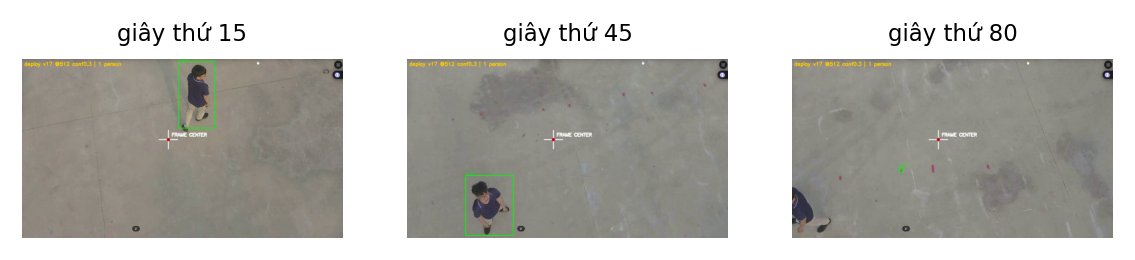
\includegraphics[width=\textwidth]{demo_khung.png}
\caption{Phần 1 của video bay thử: SteadyDet-N phát hiện người trên các khung hình của chuyến bay 21/07/2026}
\end{figure}

\begin{figure}[H]
\centering
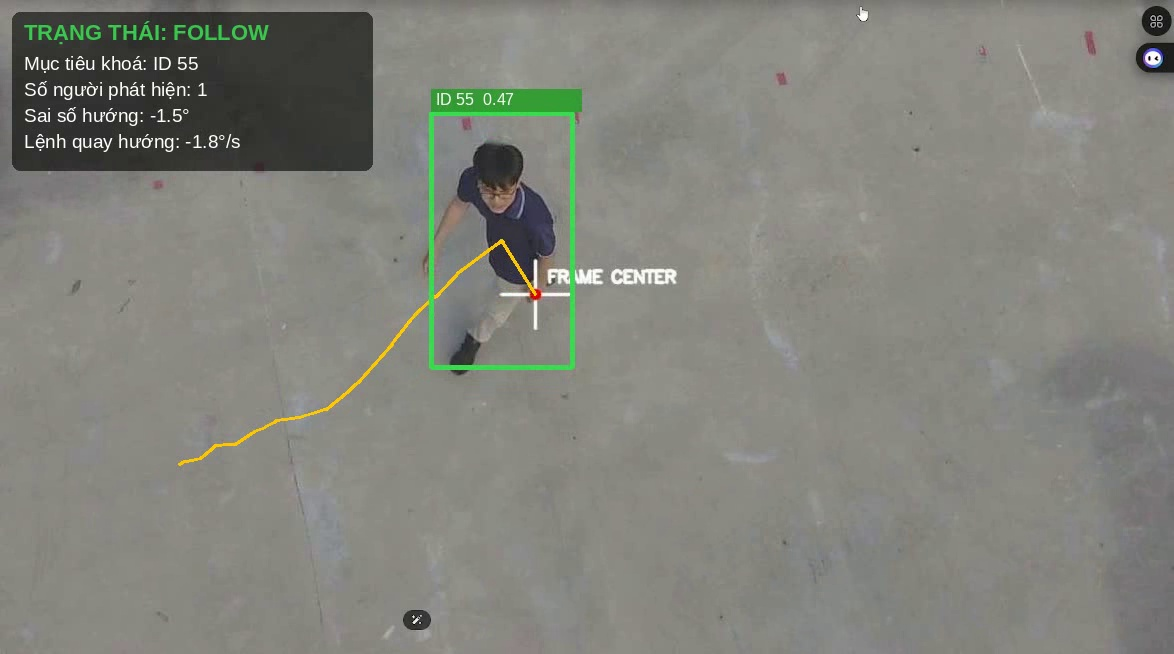
\includegraphics[width=0.8\textwidth]{vongbam_2.jpg}
\caption{Phần 2 của video bay thử: vòng bám người khoá mục tiêu, hiển thị trạng thái, sai số hướng và lệnh quay hướng}
\end{figure}

% =====================================================================
%  PHỤ LỤC E. POSTER VÀ STANDEE
%  Poster theo mẫu BM07A: in màu 1 bản A1 (báo cáo triển lãm) và 1 bản A3
%  (đóng vào cuốn báo cáo tổng kết). Standee theo mẫu BM07B.
% =====================================================================
\chapter{Poster và standee của đề tài}
\label{pl:e}

Poster của đề tài được trình bày theo mẫu BM07A/QT-PKHCN-NCKHSV/00: khổ A3 nằm ngang, bốn cột, gồm phần đầu (tên đề tài, mã số, giảng viên hướng dẫn, sinh viên thực hiện, email, khoa, logo trường và logo đơn vị), phần tóm tắt kèm từ khoá, và bốn mục I--IV cùng tài liệu tham khảo. Bản in triển lãm khổ A1 dùng cùng nội dung, phóng theo tỷ lệ 2:1 (tệp \texttt{poster\_a3/poster\_a1.pdf}).

Standee của đề tài (tệp \texttt{standee/standee.pdf}) trình bày theo mẫu BM07B/QT-PKHCN-NCKHSV/00, khổ 0,6 $\times$ 1,6\,m, gồm năm mục I--V.

Trang sau là bản poster khổ A3 đóng kèm theo quy định.
\clearpage
\IfFileExists{../poster_a3/poster_a3.pdf}{%
  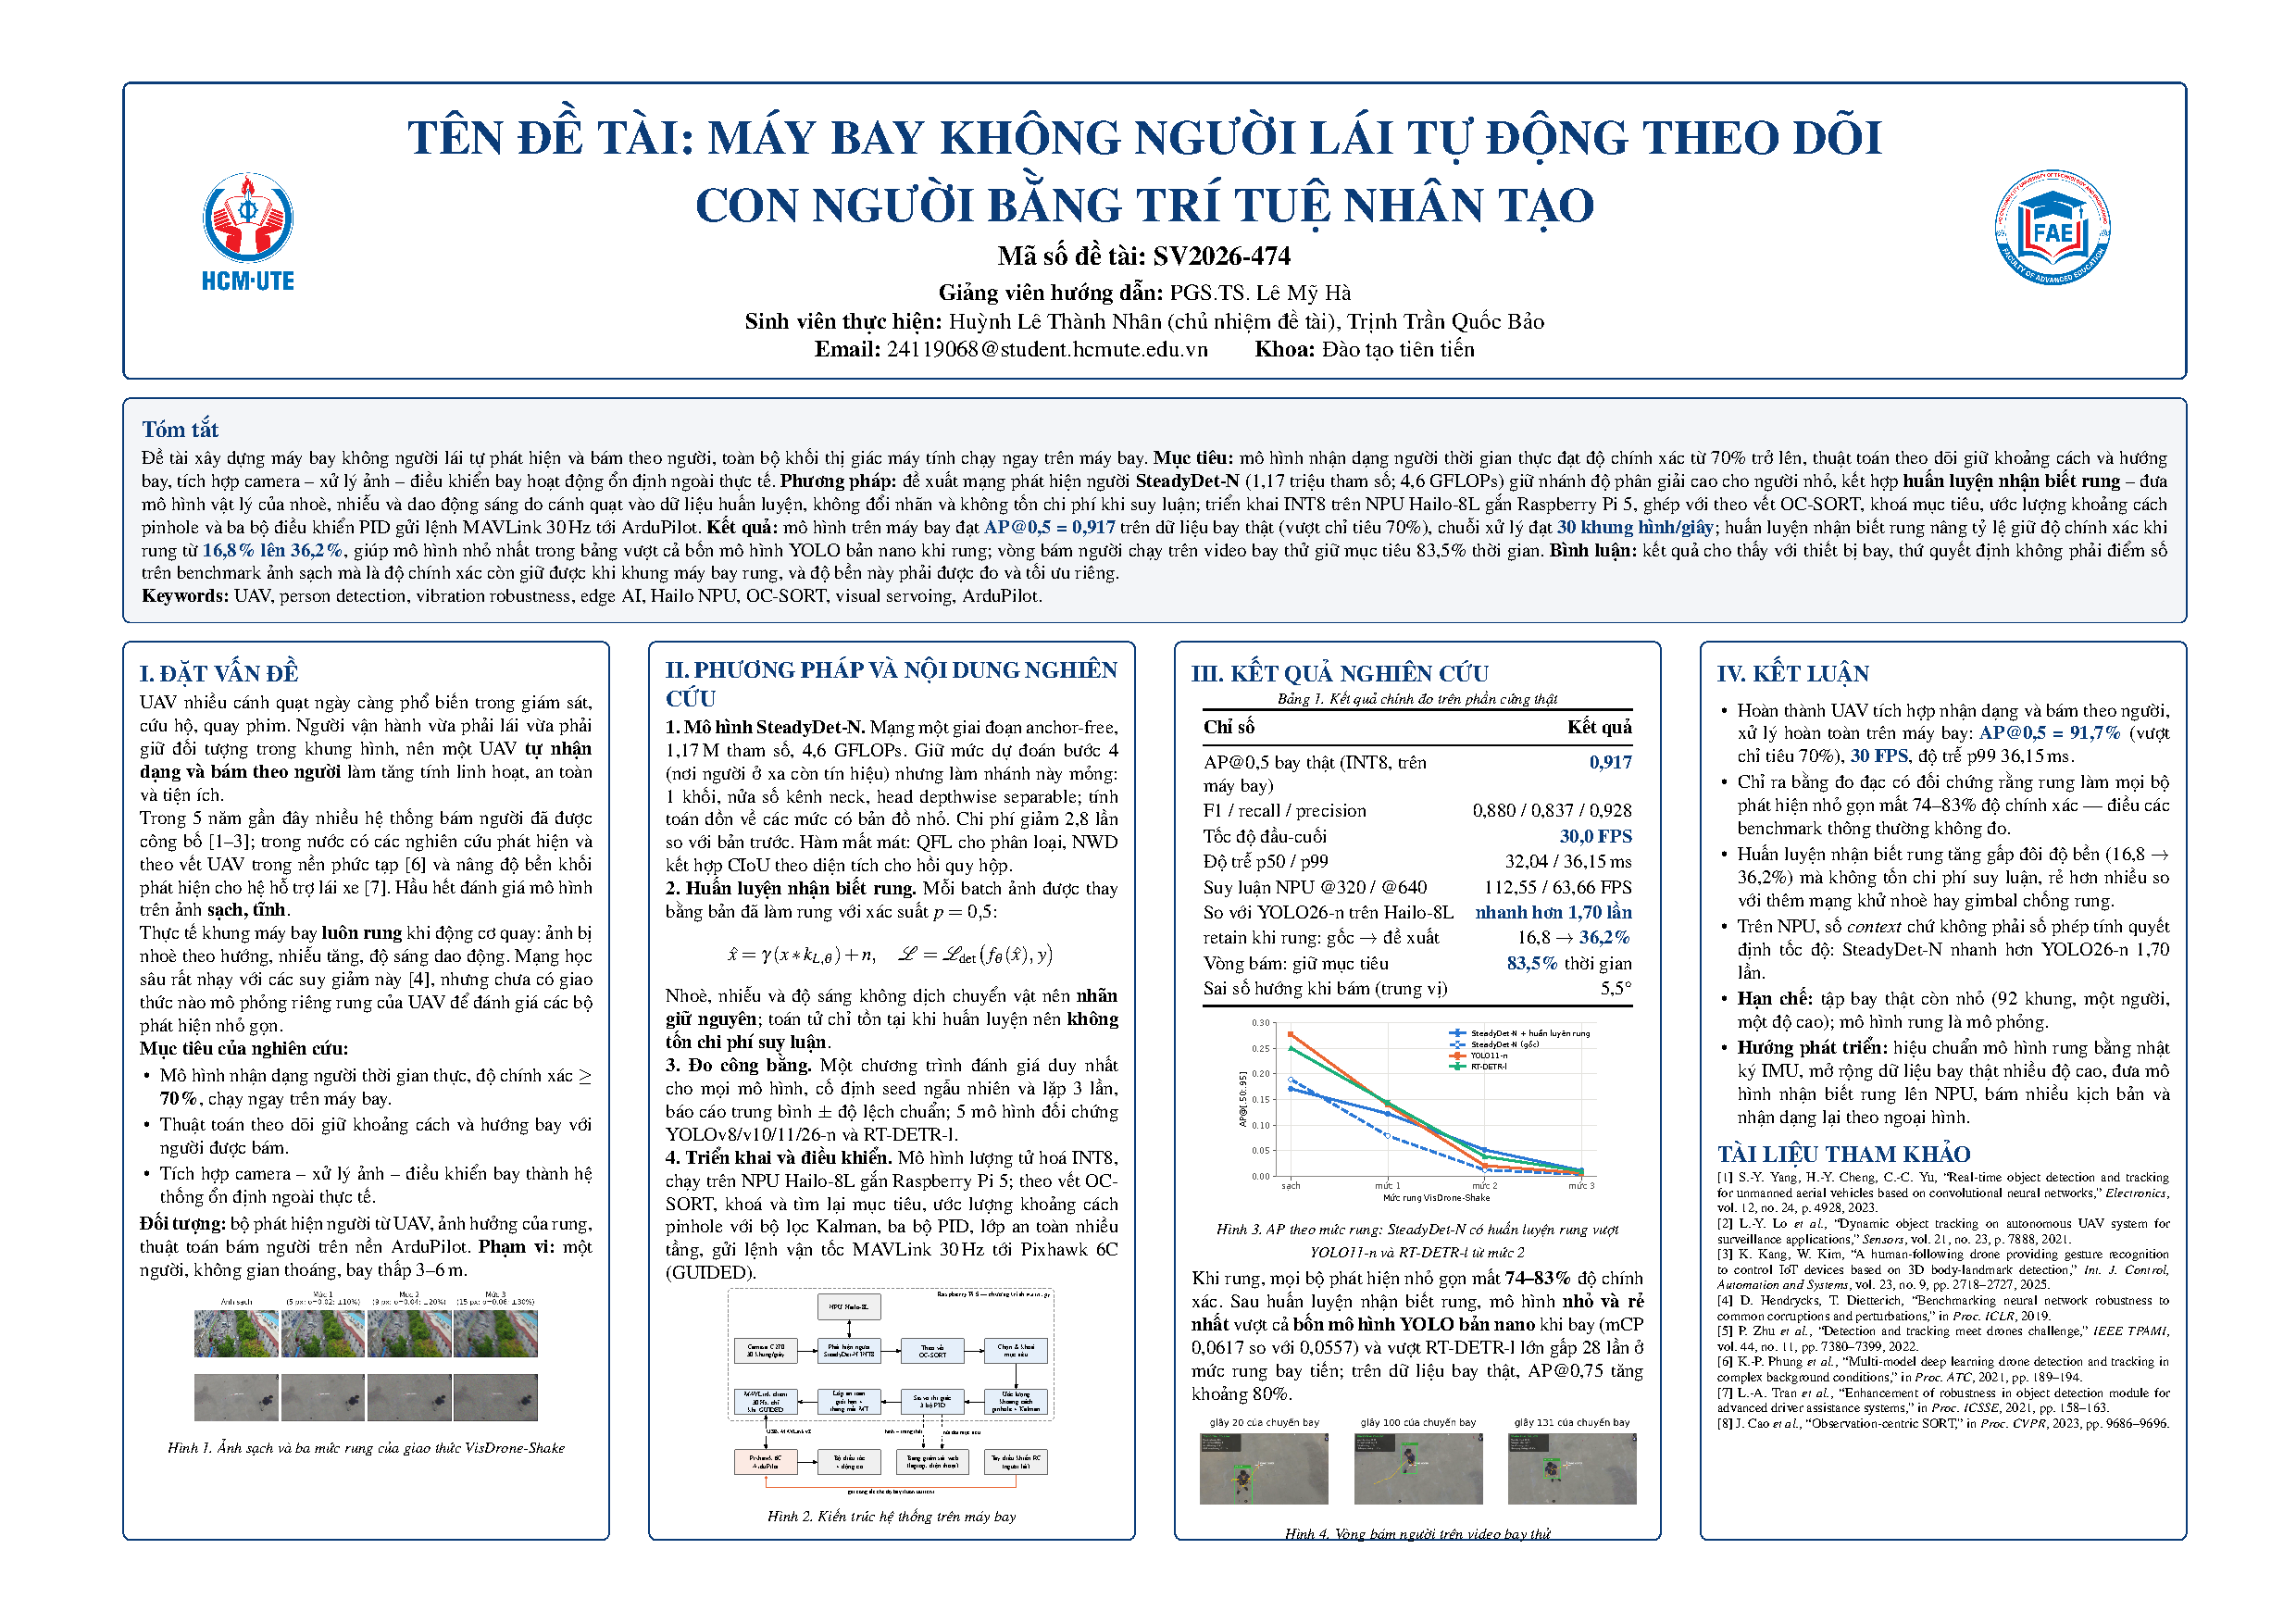
\includepdf[pages=1,angle=90,fitpaper=false,scale=0.68,
              pagecommand={\thispagestyle{empty}}]{../poster_a3/poster_a3.pdf}}{}

% =====================================================================
%  PHỤ LỤC F. BẢN SAO THUYẾT MINH VÀ HỢP ĐỒNG
%  (Phụ lục hướng dẫn, mục 3.14: đóng kèm 1 bản sao Thuyết minh và Hợp đồng
%   đã được phê duyệt vào cuối cuốn báo cáo tổng kết.)
%  Scan hợp đồng đã ký rồi lưu thành tailieu_goc/hop_dong.pdf, biên dịch lại
%  là tự động đóng vào sau thuyết minh. Nếu chưa có tệp, phần này tự bỏ qua
%  và bạn kẹp bản scan/bản photo vào cuối cuốn khi đóng quyển.
% =====================================================================
\chapter{Bản sao thuyết minh và hợp đồng đã được phê duyệt}
\label{pl:f}
Phụ lục này gồm bản sao thuyết minh đề tài nghiên cứu khoa học sinh viên năm 2026 (mẫu BM02/QT-PKHCN-NCKHSV/00, mã số \madetai) và bản sao hợp đồng thực hiện đề tài đã được phê duyệt.
\clearpage
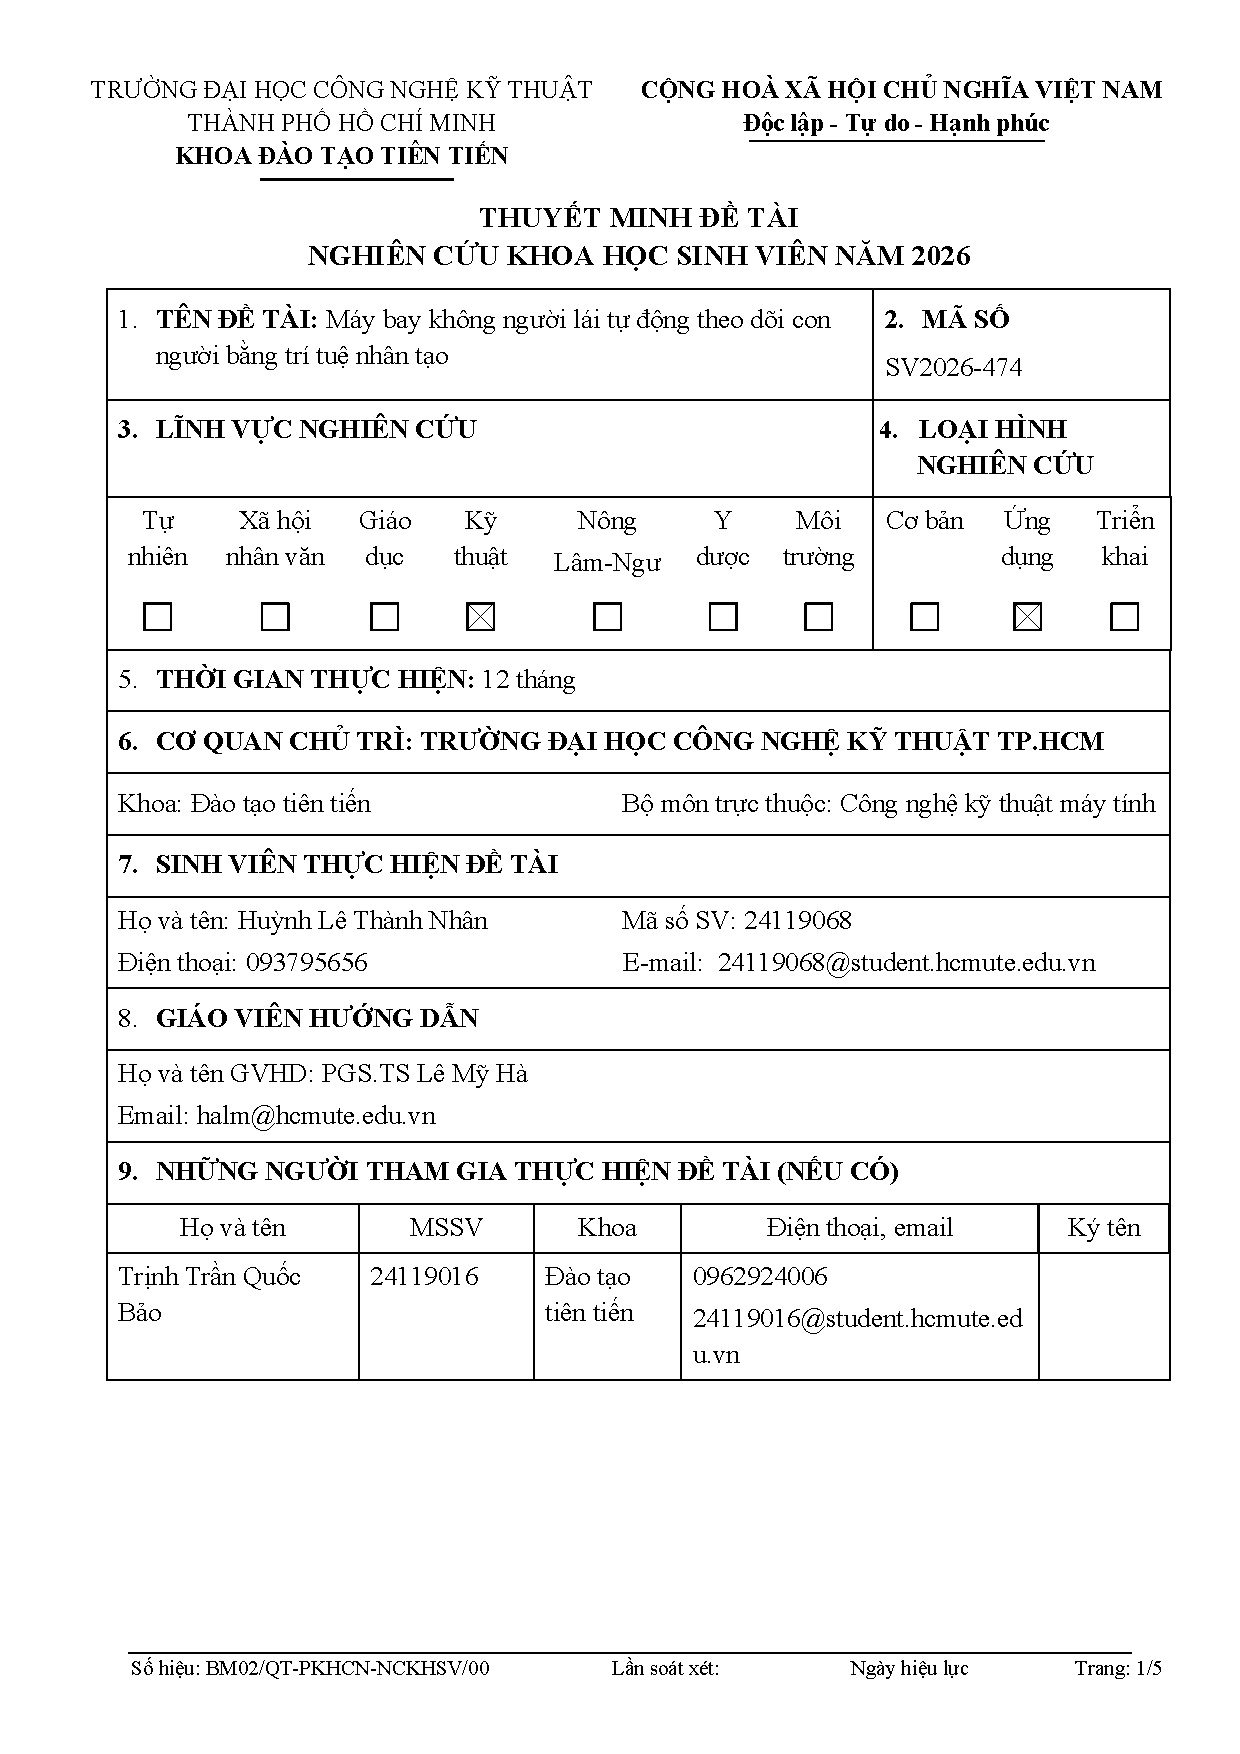
\includepdf[pages=-,scale=0.92,pagecommand={\thispagestyle{plain}}]{../tailieu_goc/BM02_NCKH_HuynhLeThanhNhan_v3.pdf}
\IfFileExists{../tailieu_goc/hop_dong.pdf}{%
  \includepdf[pages=-,scale=0.92,pagecommand={\thispagestyle{plain}}]{../tailieu_goc/hop_dong.pdf}}{}


\end{document}
